\resetfigpath{Methodology}
 


We model the behaviors of human drivers in a simplified crossroad setup as in Fig.\ref{fig:model_demo} with two vehicles. The ego vehicle is moving toward the East while the surrounding vehicle is moving toward the North. Both vehicles try to cross the intersection with no signal. Let us consider only the longitudinal states with locations and velocity along the line of action without lateral movements. The lines of movement interact at the point with the symbol $\oplus$, we define the point as \emph{the node} in this work.
\begin{figure}[htbp]
\begin{center}
%\setlength{\unitlength}{0.012500in}
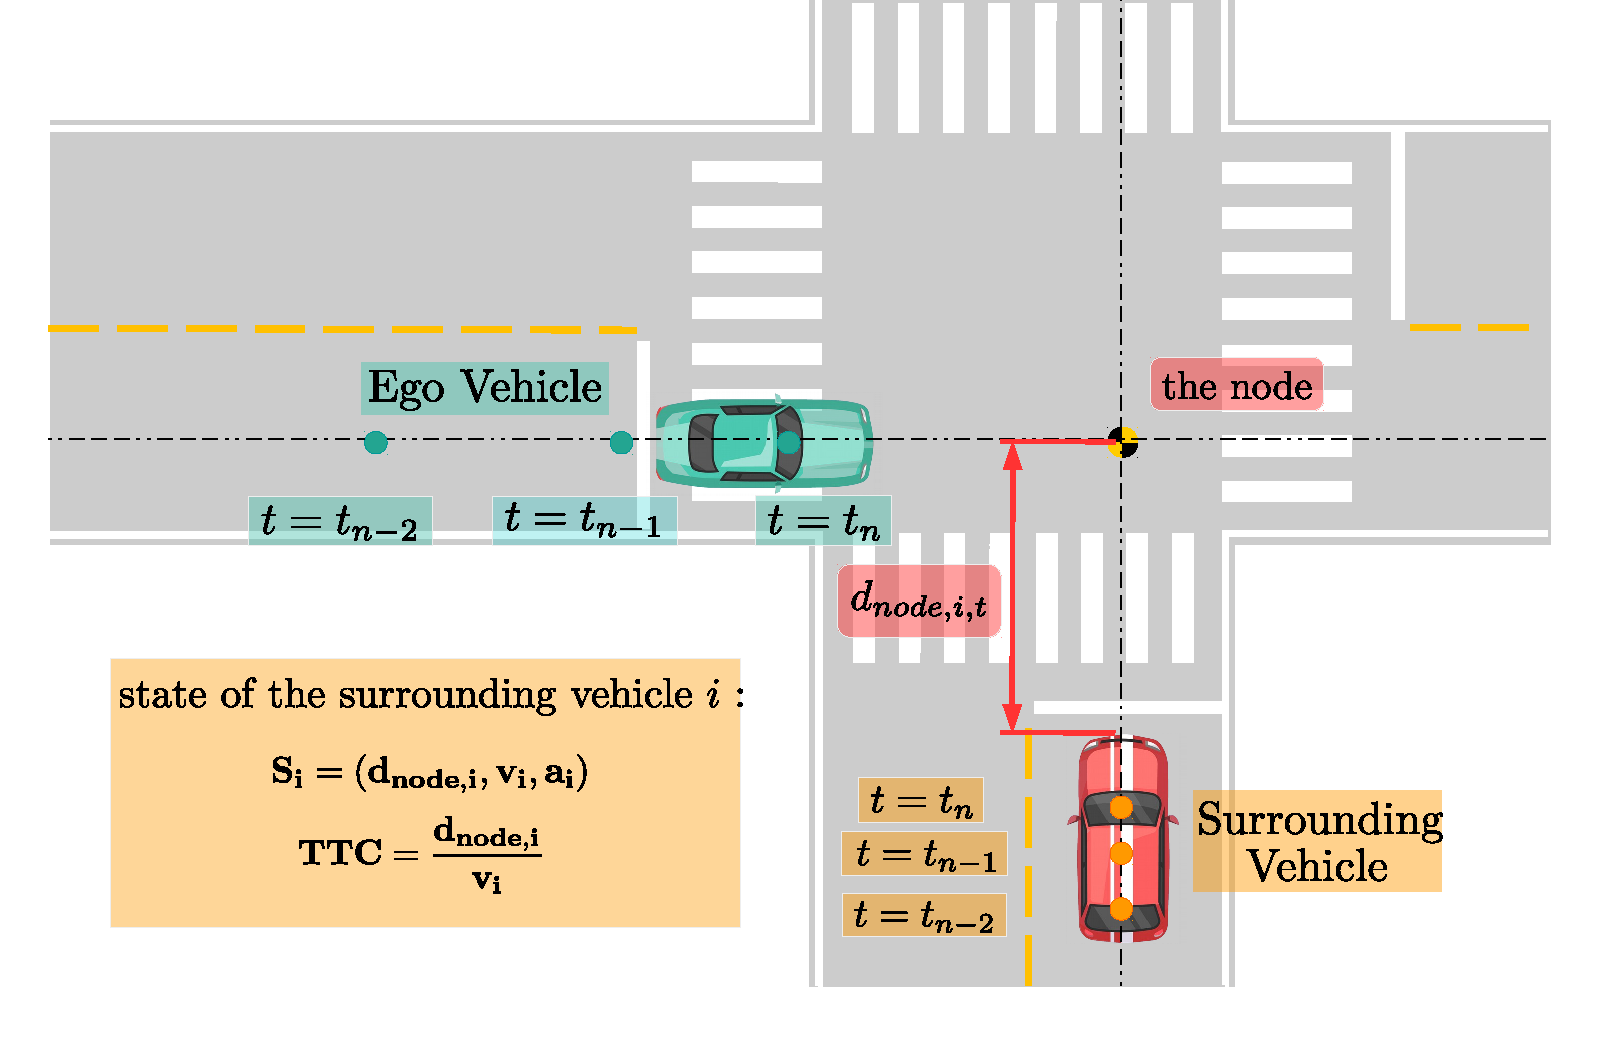
\includegraphics[scale=0.5]{intersection_concept.pdf}
\end{center}
\caption{A scenario of two vehicles passing a crossroad with no signals}
\label{fig:model_demo} 
\end{figure}

Let the node be the origin of the coordinate system with the velocity of the ego vehicle along the positive $x$ direction, the velocity of the other agent along the positive $y$. The distance from the position of the $i$th vehicle at time $t$ to the node is $d_{\mathrm{node}, i}(t)$. $v_i(t)$ and $a_i(t)$ are the speed and the acceleration of the vehicle $i$ at time $t$, respectively. The states of each $i$th vehicle are defined as in Eqn.(\ref{eq:state}). 
\begin{equation}
\mathbf{S}_i(t) = \left( \begin{array}{c} d_{\text{node},i}(t) \\ 
v_i(t) \\ 
a_i(t) 
\end{array} \right) 
\label{eq:state}
\end{equation}

The decision process on passing or yielding of the ego vehicle is shown in Fig.\ref{fig:decision_map}. At each time instance, the states of the ego vehicle and the states of another agent are obtained. All these information are used to determine if a potential treat is present. The ego vehicle proceed with no threats, and take appropriate actions when threats are predicted. The concepts of time to collision and time for action are both introduced as the mechanisms drivers employed to determine avoid potential collisions. Apparently the time for action vary between drivers and between occasions, we therefore use probability distributions to estimate the probability of braking in Section \ref{subsec:TFADistribution}, followed by a probabilistic evaluating model in Section \ref{subsec:MathModel}. Experiments at both simulated and real environment are described in Section ~\ref{subsec:ValidatePOY}.
\begin{figure}[htbp!]
\begin{center}
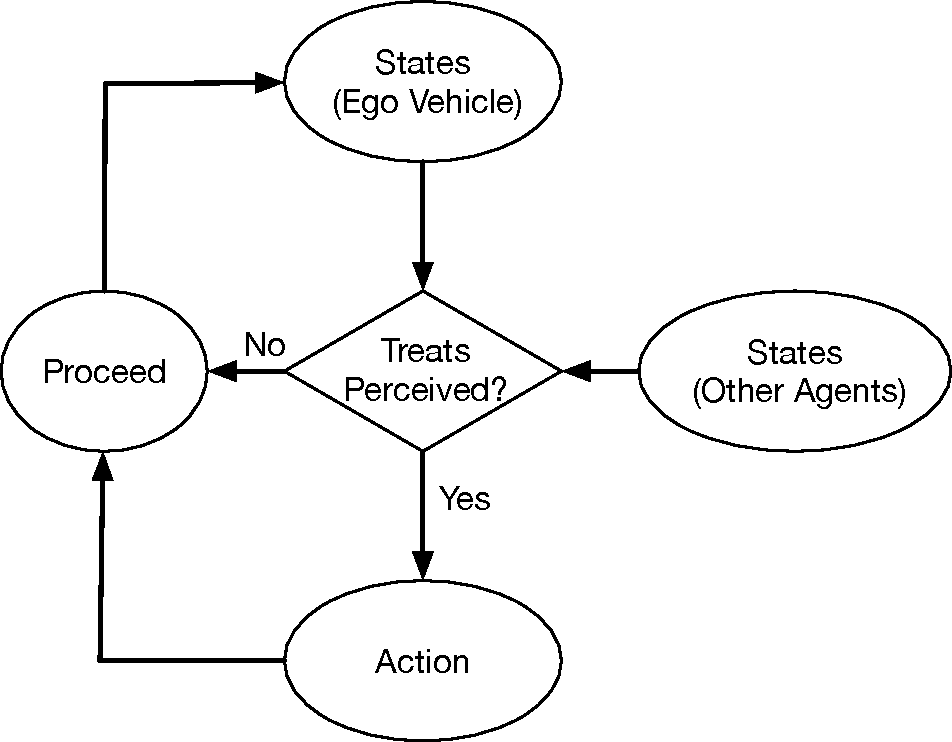
\includegraphics[scale=0.63]{Methodology/figs/Decision_Map.pdf}
\end{center}
\caption{Pass-or-yield decision map for the ego vehicle.}
\label{fig:decision_map} 
\end{figure}





%We develop a model that is able to account for human driver behaviors is required. Since the targeted model should rely heavily on the interaction among traffic participants, the unsignalized crossroads are chosen as the scenario that the model build around for the fact that it is the most communication-requiring traffic scenario, where the other participant's intentions to pass or yield are essential for one to cross safely.



%%%%%%%%%%%%%%%%%%%%%%%%%%%%%%%
\subsection{Time to Collision}

\ac*{TTC}, or time to contact, quantifies the predicted time to collide with an obstacle ahead\cite{Caird1994}. In traffic safety assessments, TTC is described as “the time required for two vehicles to collide if they continue at their present speed, and on the same path” by Hayward\cite{Hayward1972}. Experiments by Cavallo et al. in \cite{TTC} also showed that TTC as described in Eqn.(\ref{eq:TTC_dv}) properly drivers at different ages, genders, and experience levels when obstacles are encountered. 

%We use the definition of TTC in Eqn.(\ref{eq:TTC_dv}) with the information about the speed and the distance to the node.
\begin{equation}
TTC = \frac{\text{distance to the node}}{\text{speed}}=\frac{{d_{\mathrm{node},i}}}{v_i}
\label{eq:TTC_dv}
\end{equation}
Note that $d_{\mathrm{node},i}$ in Eq.(\ref{eq:TTC_dv}) is positive before passing the node and negative after passing the node.


% Although TTC  was originally applied to car following problems, Eqn.\ref{eq:TTC_tau} shows our use of TTC, in understanding human driver behaviors at crossroads.   
% \begin{equation}
% TTC = \frac{\theta_1}{(\theta_2 - \theta_1)/(t_2 - t_1)}
% \label{eq:TTC_tau}
% \end{equation}
% The optic variable $\tau_{optic}$ in Eqn.(\ref{eq:TTC_tau}) is the inverse of the rate of dilation of the object relative to the observer. $\theta_1$ and $\theta_2$ are the angular distances of the obstacle's image on the retina at times $t_1$ and $t_2$ separately. Hence the $(\theta_2 - \theta_1)/(t_2 - t_1)$ would be the expansion rate of the obstacle as the observer approaches. However, since both empirical results and analyses suggest that the hypothesis is false, there has been intense disputations over whether $\tau_{optic}$ provides necessary TTC information \cite{tau}. 

%Let $\mathbf{S}_i$ be the states of the $i$th surrounding vehicle that ego vehicle observed, TTC can then be estimated using the distance to the node and the current speed of the vehicle as in Eqn.(\ref{eq:TTC_crossroad}) by combining Eqn.(\ref{eq:state}) and Eqn.(\ref{eq:TTC_dv})  
% \begin{equation}
% \mathrm{TTC} = 
% \label{eq:TTC_crossroad}
% \end{equation}

%represents the \textit{displacement} for the purpose of separating the states before and after passing the node in later figures. Throughout this research, however, the use of displacement and distance are interchangeable since the situations that we are interested in happen before reaching the node (i.e. the displacement is always positive).

%%%%%%%%%%%%%%%%%%%%%%%%%%%%%%%
\subsection{Time for Action}

The mechanism of pass-or-yield decision process of both drivers in Fig.\ref{fig:model_demo} unconsciously used by human drivers is defined using the parameter ``\ac*{TFA}``. TFA plays a critical role in the braking decision process by serving as a braking probability indicator of drivers. Fig. \ref{fig:TTC_brake_comb} illustrates an example similar to the time-history of braking in \cite{time_history}. On the top of Figure \ref{fig:TTC_brake_comb} we have an ego vehicle approaching from the left and trying to avoid the collision at the node on the other end. At the point $P_A$, the car is cruising with the velocity $v_i$. The driver might have observed the obstacle at $P_A$, but determined not to take actions. Moving forward to $P_B$ when the driver realized imminent danger and then applied the brake. The vehicle slows down and finally comes to a stop with the speed equals to $0$ at point $P_C$. The velocity profile and the pressure on the brake in Fig.\ref{fig:TTC_brake_comb} record the actions about the driver. 

\begin{figure}[htbp!]
\begin{center}
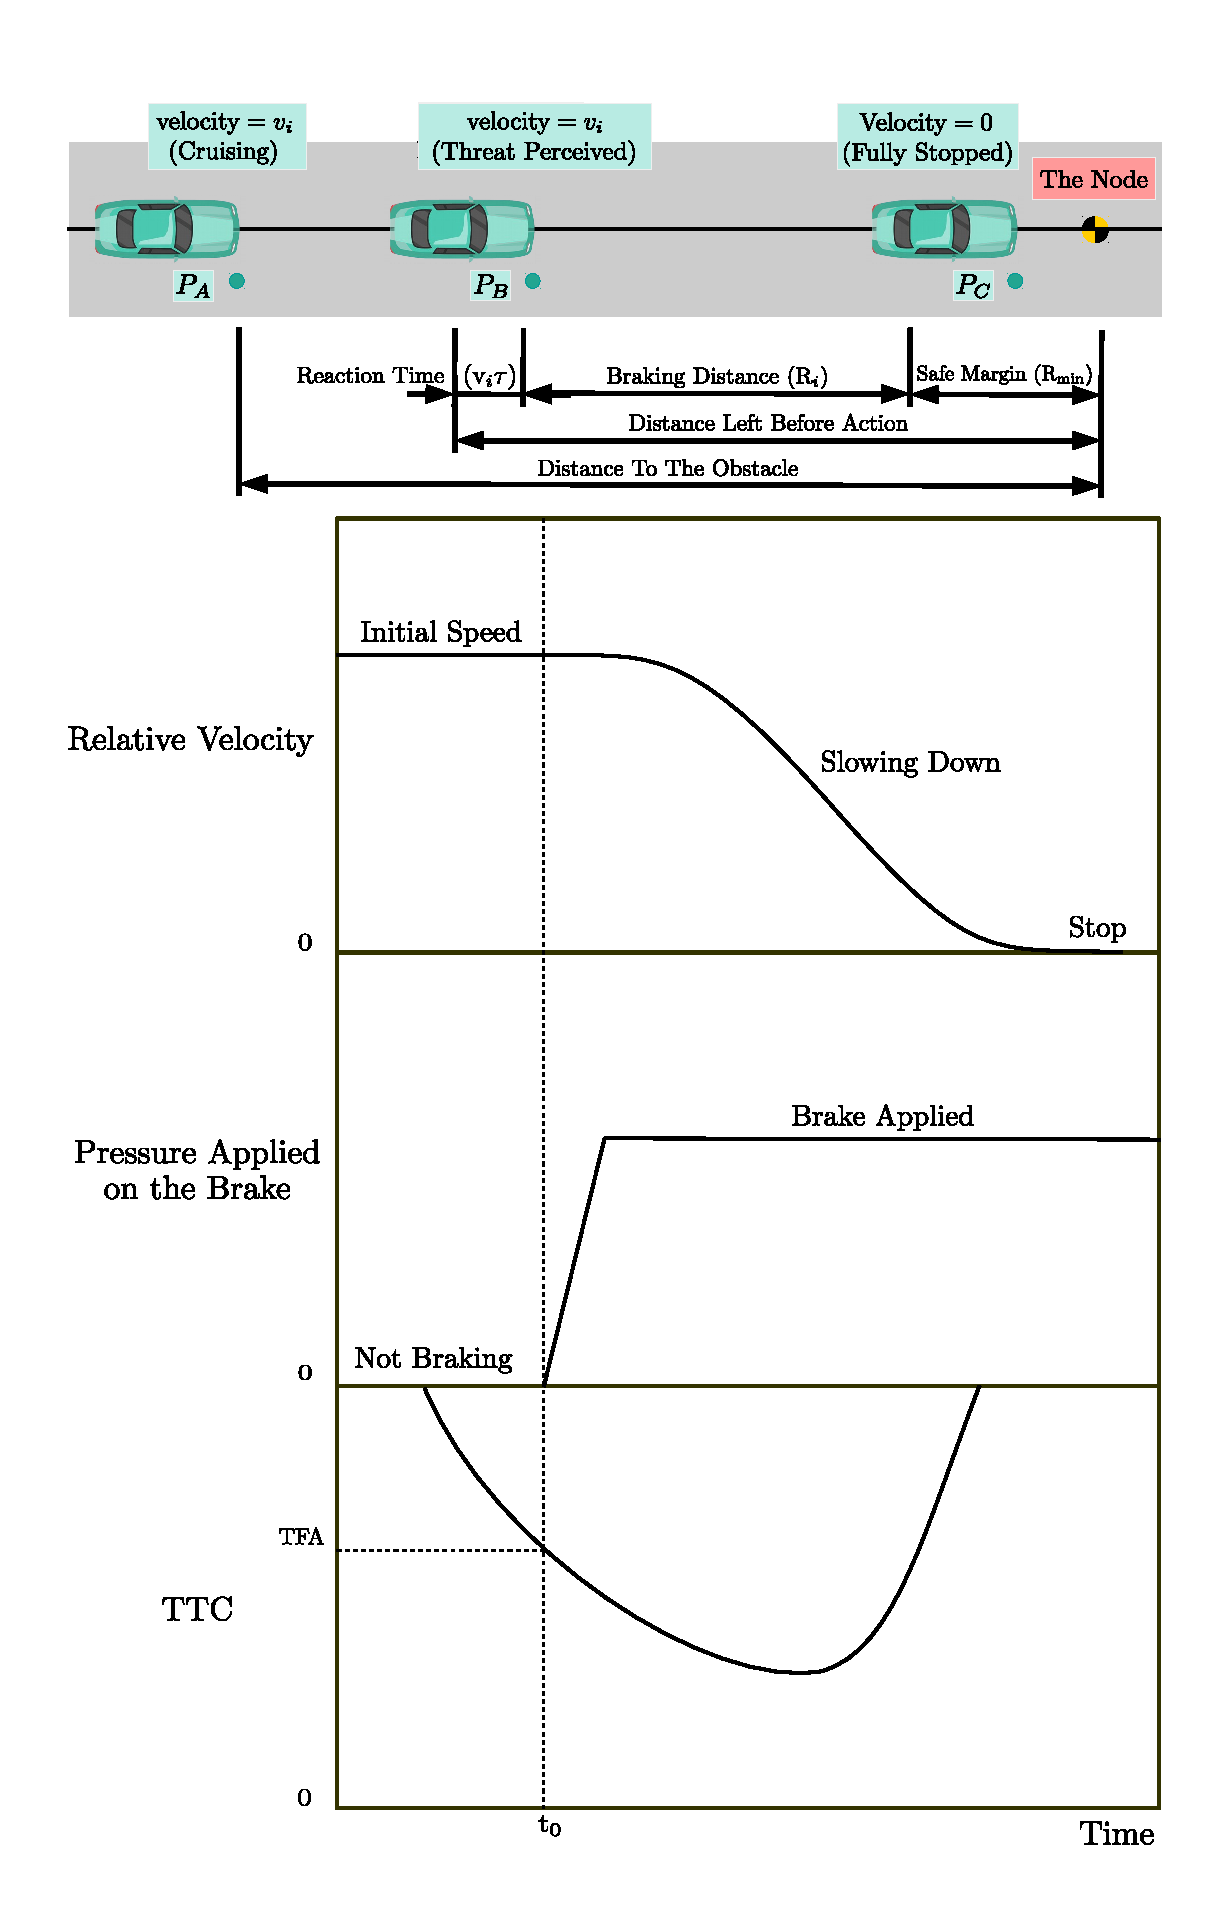
\includegraphics[scale=0.63]{TTC_change_braking_comb.pdf}
\end{center}
\caption{History of time to collision when brake is applied.}
\label{fig:TTC_brake_comb} 
\end{figure}
Let us look at the bottom of Fig.\ref{fig:TTC_brake_comb} as TTC decreases as the distance to the obstacle is getting shorter. The braking decision is made at point $P_B$ resulting a full stop at $P_C$. Let us consider the distance from $P_B$ to the obstacle the minimum distance required to avoid collision, the time driver has to take action to avoid collision is the minimum distance divided by vehicle velocity $v_i$, this is defined as "Time for Action (TFA)". 

TTC provide drivers a reference of when the potential collision with the obstacle might happen. The driver will hit the brake to avoid potential collision at the moment that TTC equals to TFA. This process could also be applied to the crossroad scenario when two vehicles are about to arrive at the node simultaneously. In this situation, it is foreseeable for both drivers to avoid the collision that will happen at the node, just like knowing the collision which will happen at the end of the road with the obstacle in Fig.~\ref{fig:TTC_brake_comb}. Since the node is the only a point on the intersection of these two perpendicular paths , situations for both drivers are similar to that described in Fig.~\ref{fig:TTC_brake_comb}. 


% (as shown in Fig.~\ref{fig:imagine_obstacle})
% \begin{figure}[htbp!]
% \begin{center}
% 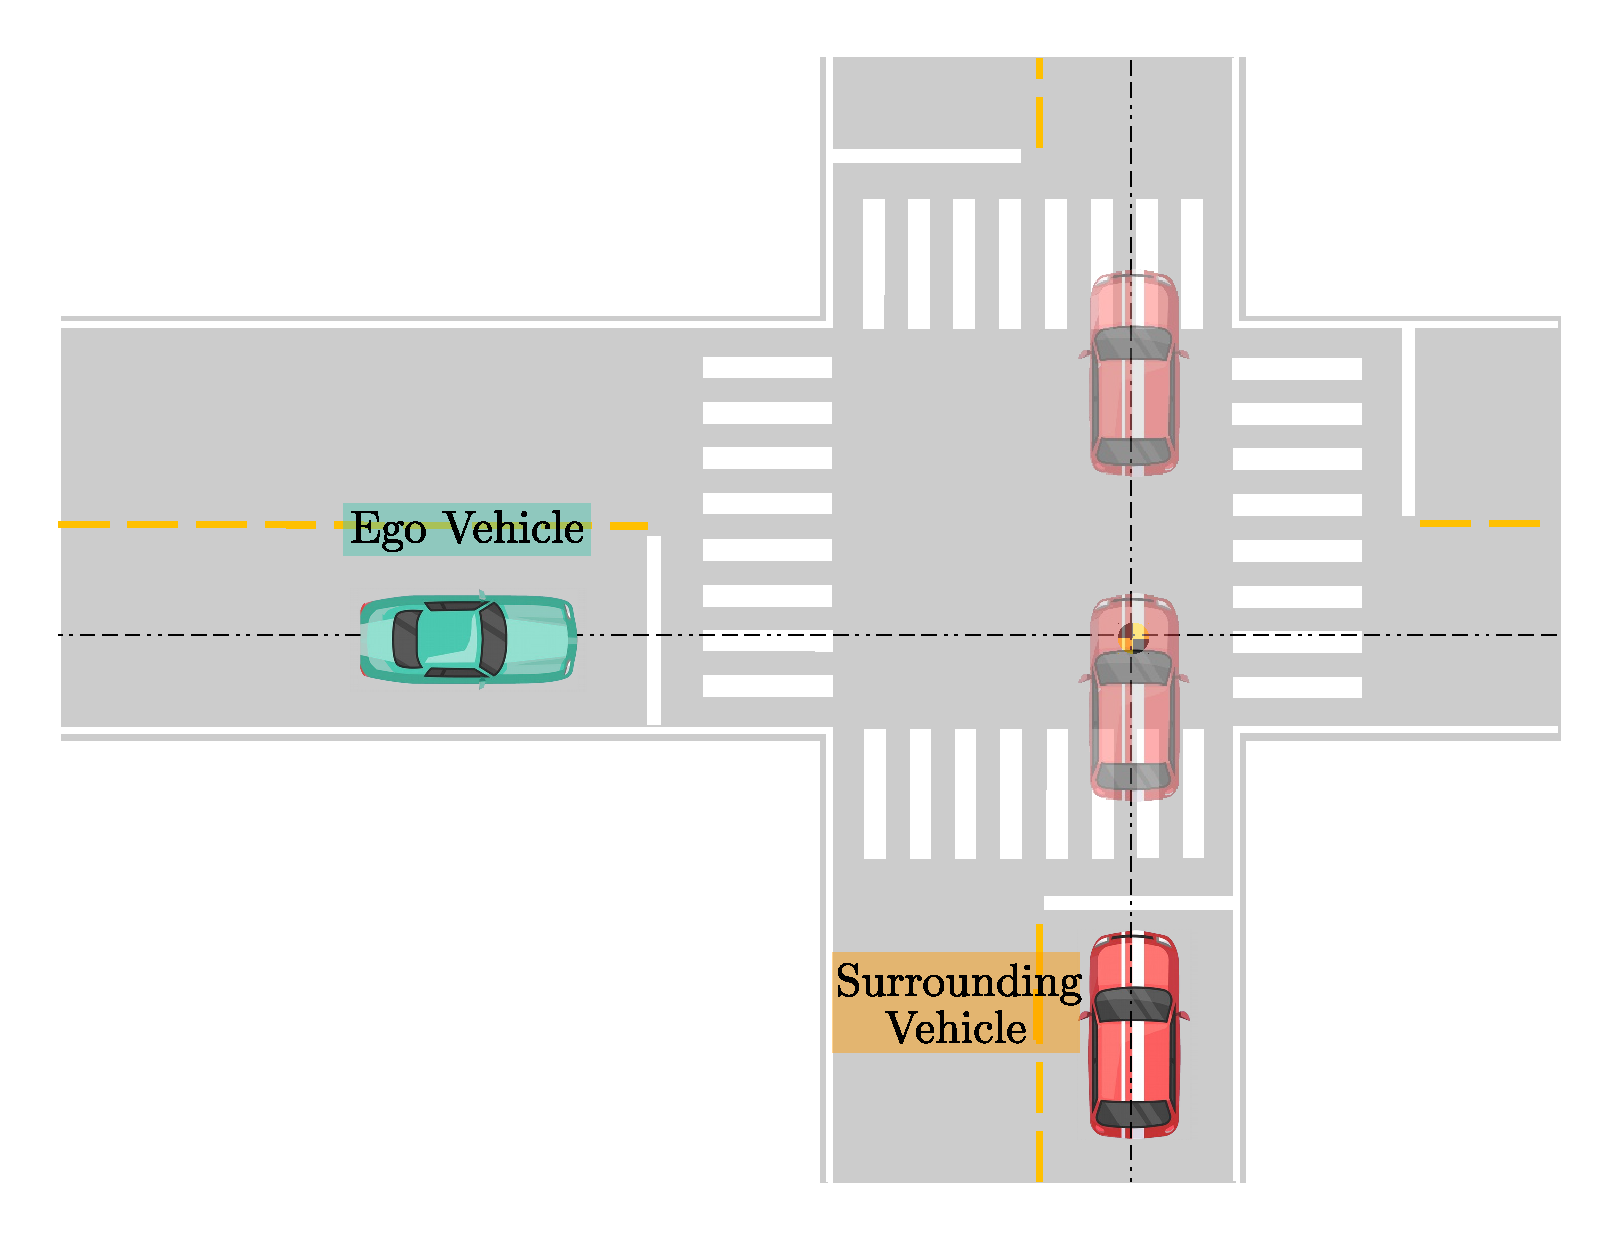
\includegraphics[scale=0.43]{intersection_imagining_obstacle.pdf}
% \end{center}
% \caption{The ego vehicle estimate the possible position of the surrounding vehicle depending on its current states. To avoid the potential collision, the ego vehicle adjust the time to brake as if the oncoming vehicle is at the intersection.}
% \label{fig:imagine_obstacle} 
% \end{figure}


%%%%%%%%%%%%%%%%%%%%%%%%%%%%%%%%%%%%%%%%%%%%%%%%%%%%%
%%%%      SUBSECTION SUBSECTION SUBSECTION       %%%%   
%%%%%%%%%%%%%%%%%%%%%%%%%%%%%%%%%%%%%%%%%%%%%%%%%%%%%


\subsection{The TFA Distribution}
\label{subsec:TFADistribution}

The TFA represents a specific TTC drivers decide to take actions, as depicted in the bottom of Fig.\ref{fig:TTC_brake_comb}. Under the most ideal situation, a driver avoids collisions by braking exactly at his/her TFA, which is the two-dots-dashed line in Fig.\ref{fig:TFA_driver_general}. However, due to variations of human perceptions and operations, drivers only act according to current circumstances and brake somewhere close to but not exactly equal to the TFA of the driver. Hence, if we collect all the observed TFAs of a driver when he or she brakes to avoid obstacles, the two-dots-dashed lines in Fig.\ref{fig:TFA_driver_general} would turned into the area with slash lines in Fig.\ref{fig:TFA_driver_general}) as the TFA uncertainty during braking. 


\begin{figure}[htbp!]
\begin{center}
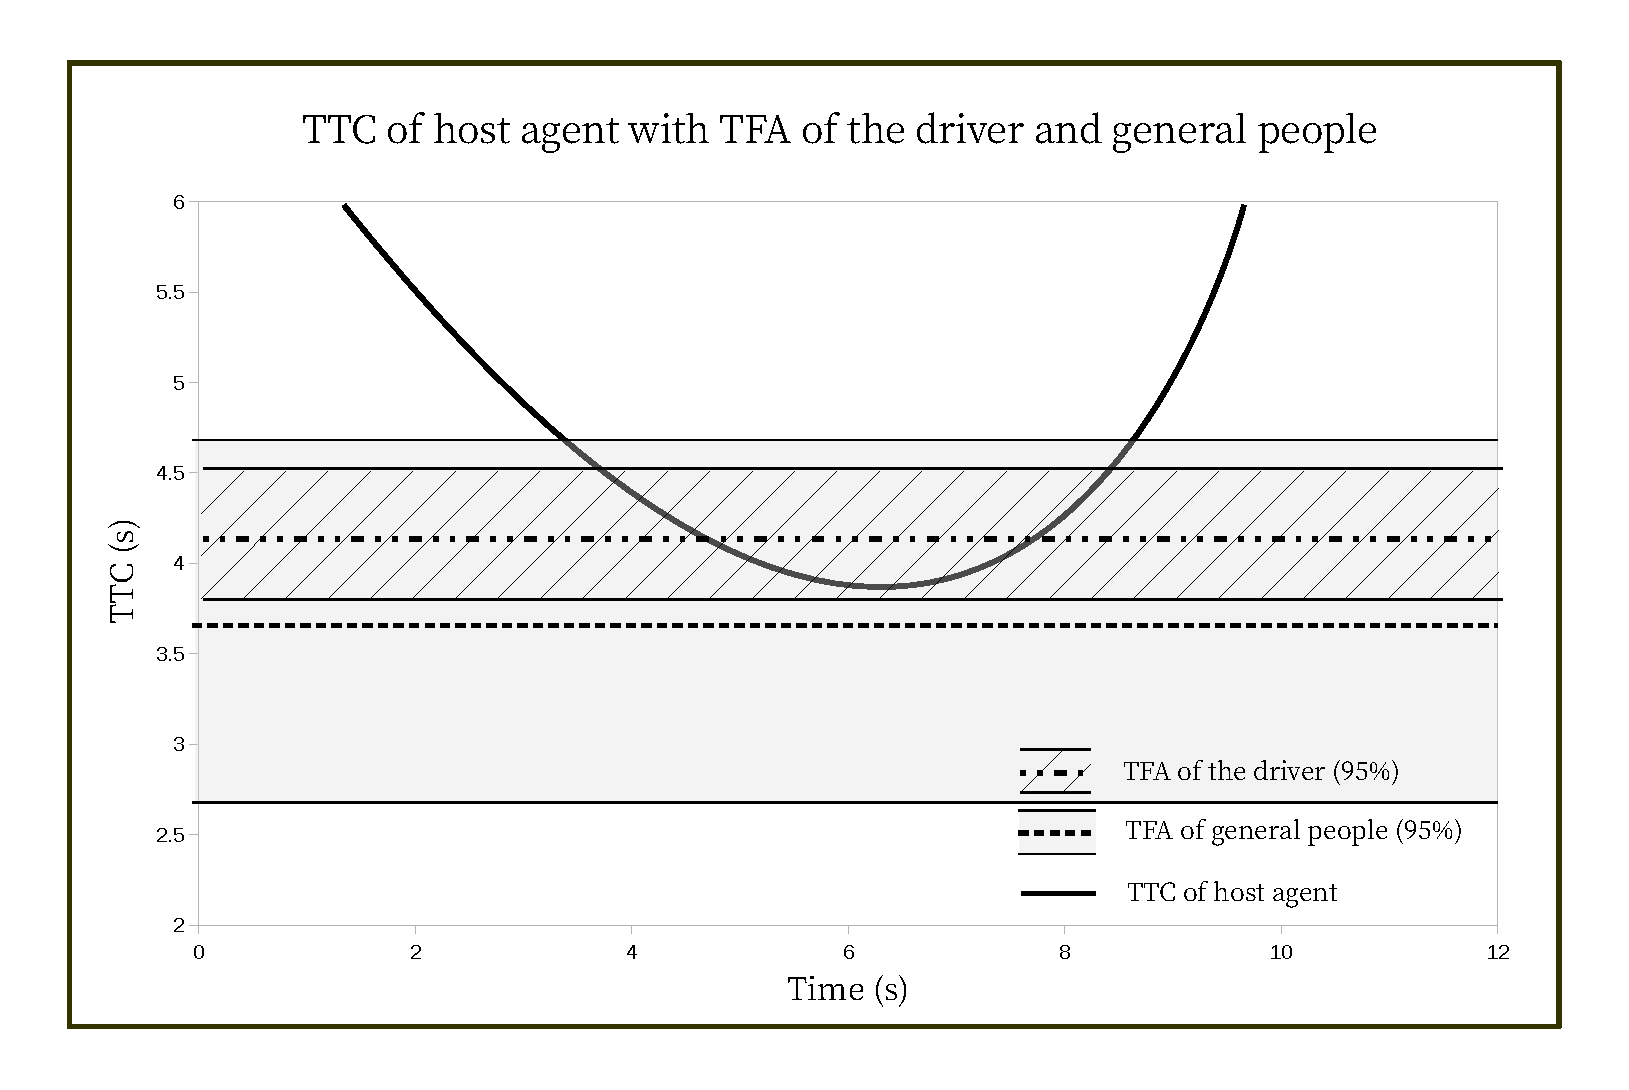
\includegraphics[scale=0.5]{TFA_distribution_driver_and_general.pdf}
\end{center}
\caption{Example of TFA of the driver, TFA of general people and TTC of the ego vehicle.}
\label{fig:TFA_driver_general} 
\end{figure}

% \begin{figure}[htbp!]
% \begin{center}
% 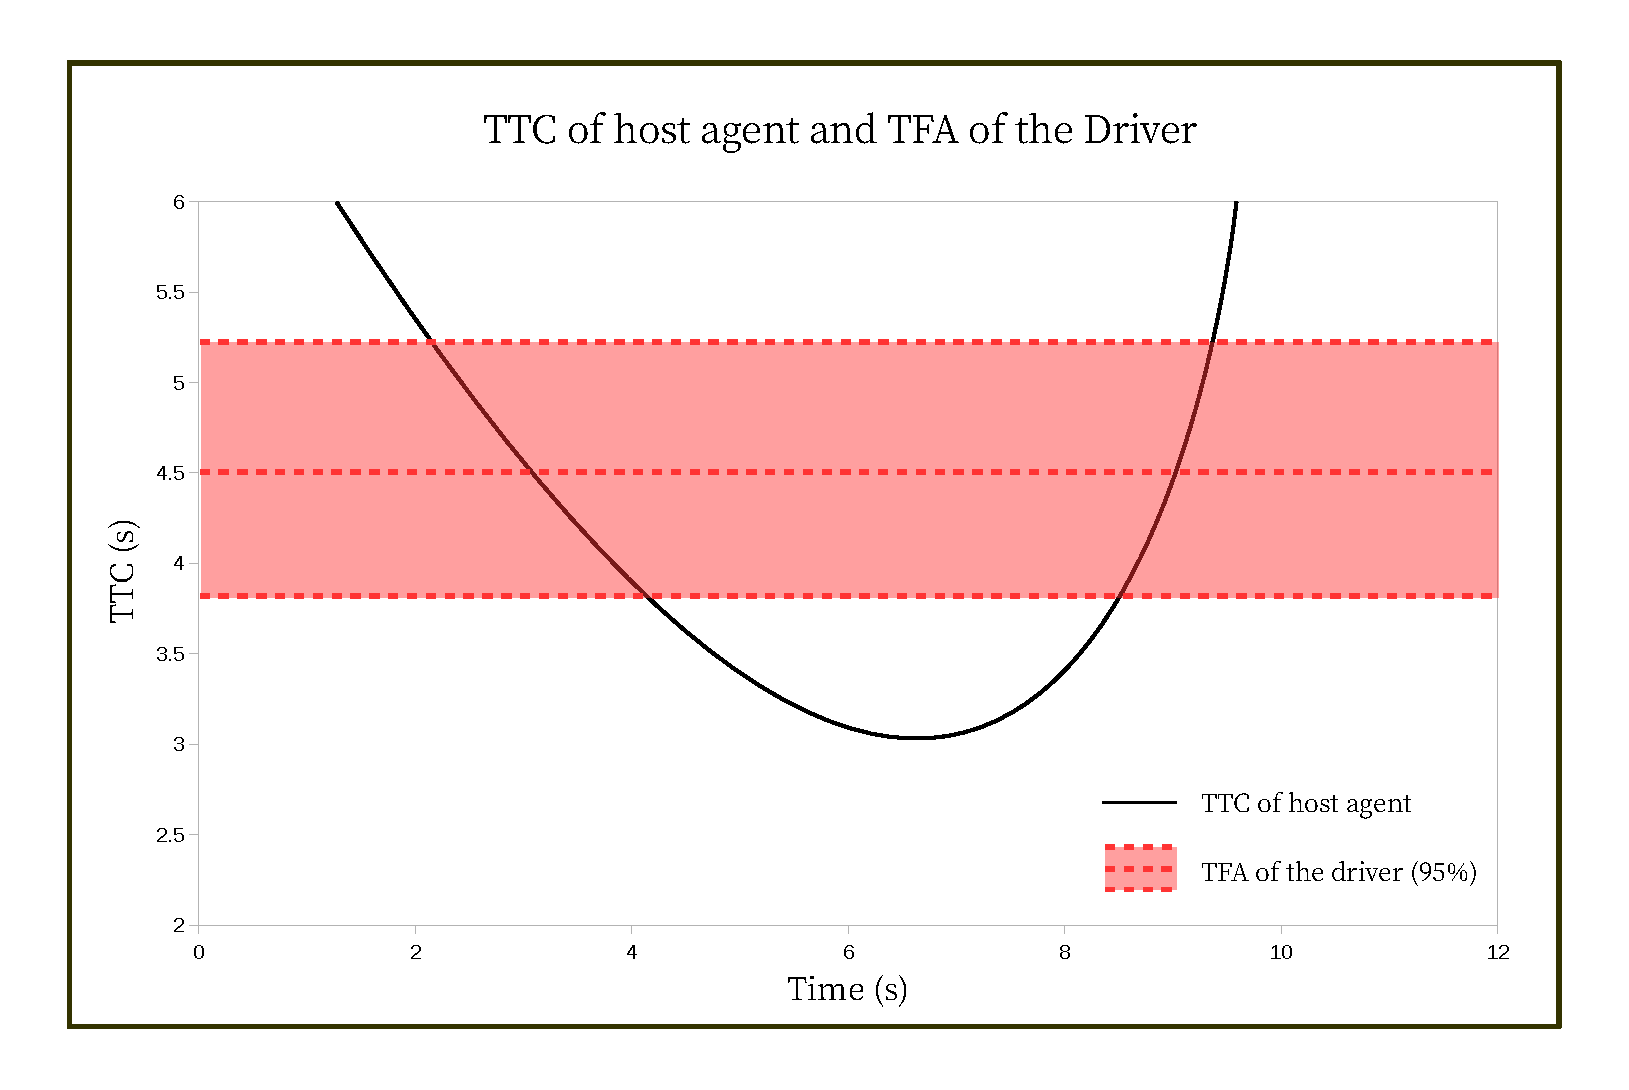
\includegraphics[scale=0.5]{TFA_distribution_driver_example.pdf}
% \end{center}
% \caption{Example of TFA distribution of the driver and TTC of the ego agent.}
% \label{fig:TFA_distribution} 
% \end{figure}

The TFA of all drivers shall extend the TFA distribution of a single driver to a wider range to reflect inter-driver differences such as risk-taking levels as well as responses in all scenarios. For example, an aggressive driver with a high performance sports car might have a relatively low TFA because of his personality and the short braking distance of the performance car; on the contrary, a rookie driver in an old passenger sedan might have a higher TFA with longer stopping distance. Other factors such as the state of mind when driving and reaction time could also affect TFA of a driver. The TFA distribution suggests that``within this range of TTC, some drivers will initiate the action (of braking) if potential collisions exis``. The gray band area in Fig.~\ref{fig:TFA_driver_general} illustrates the case when 95\% of people's TFAs are within 1.5 to 4.5 seconds with the mean value indicated by the dashed line, considering both the TFA uncertainty during braking and the TFA differences among drivers. The TTC of the ego vehicle adopted from Fig.\ref{fig:TTC_brake_comb} is shown with a curved line. We can see that when two vehicles approach a crossroad interactions, the TTC of both drivers are reducing while the chances of braking to yield is getting higher. 

We use probabilistic decision-making in modeling the interactions of two vehicles passing a crossroad. The TFA distribution with 95\% interval in Fig.~\ref{fig:TFA_driver_general} can be re-illustrated into a probability density function (PDF), as shown in Fig.~\ref{fig:TTC_distribution}. At a certain value of TTC the probability of braking can promptly be obtained via integrating the PDF. For example, for a case when the TTC of a vehicle towards a crossroad is 3, the probability for the driver to brake would then be the area to the right under the PDF, which is 50\%. Drivers with TFA greater than 3 would have braked before the TTC reached 3, because the displacement to the node is decreasing and the TTC drops as the ego vehicle is driven toward the crossroad according to Eqn.(\ref{eq:TTC_dv}), which suggests rising of the collision risk. Hence, as the TTC gets lower, the chance for the driver to brake will increase.

The first intention to brake lies on the lowest value on the TTC curve of the ego vehicle. Let us focus on the bottom of Fig.~\ref{fig:TTC_brake_comb} as in Fig.~\ref{fig:TTC_TFA_indicator}. We select three samples at $t=3$ seconds (squared), $t=5.5$ seconds (triangle), and $t=7$ seconds (circle). The corresponding values on the TFA distribution are shown in Fig.~\ref{fig:TTC_distribution}. At $t=3$ seconds the TTC of the ego vehicle is around 4.2 seconds. We can then estimate the probability of the vehicle stopping from the PDF in Fig.~\ref{fig:TTC_distribution} as 0.13\%. This result is reasonable since the TTC at this moment is still far from the TFA average. Similarly, when the $t=5.5$ seconds with TTC being 3.1, the probability of the vehicle stops increases to 40.1\%. At $t=7$ seconds, since the brake is already applied, the increases in TTC will not alter the value of probability of braking. In the scenario of Fig.~\ref{fig:TTC_TFA_indicator} and Fig.~\ref{fig:TTC_distribution} the probability of the ego vehicle braking calculated using the lowest value on the TTC is 40.1\%.

\begin{figure}[htbp!]
\begin{center}
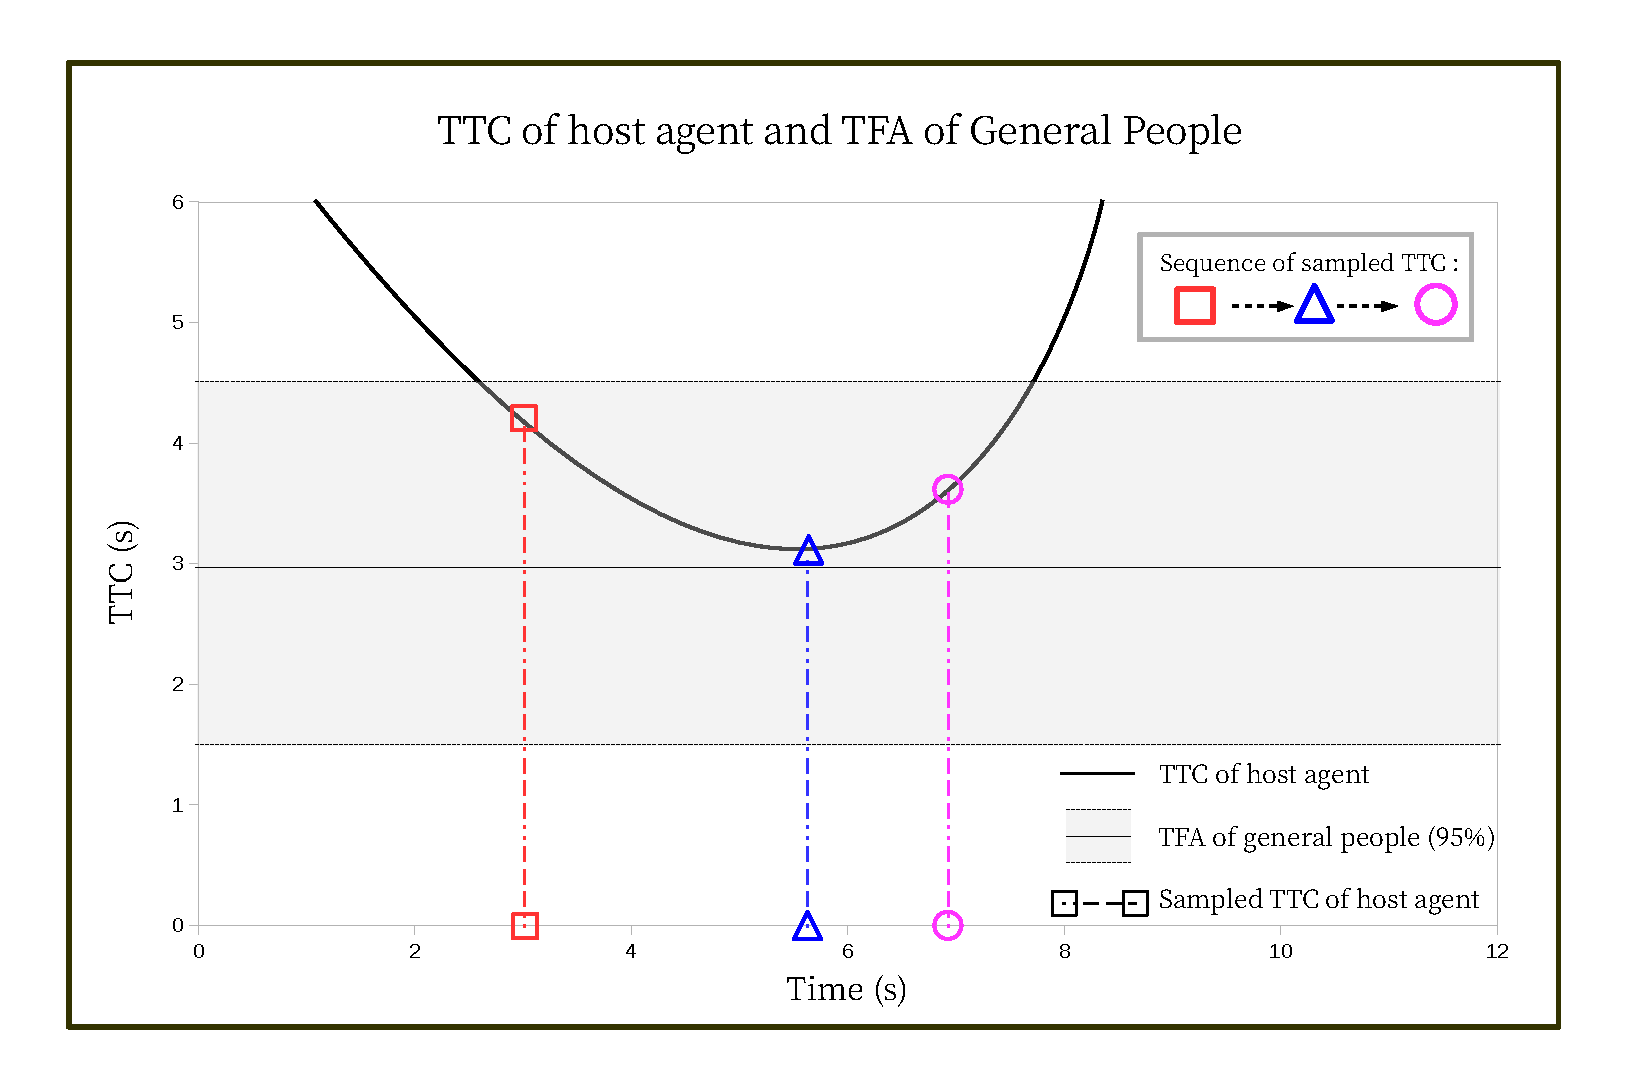
\includegraphics[scale=0.5]{TTC_probability_indicator.pdf}
\end{center}
\caption{Example of TFA of general people and TTC of the ego vehicle.}
\label{fig:TTC_TFA_indicator} 
\end{figure}

\begin{figure}[htbp!]
\begin{center}
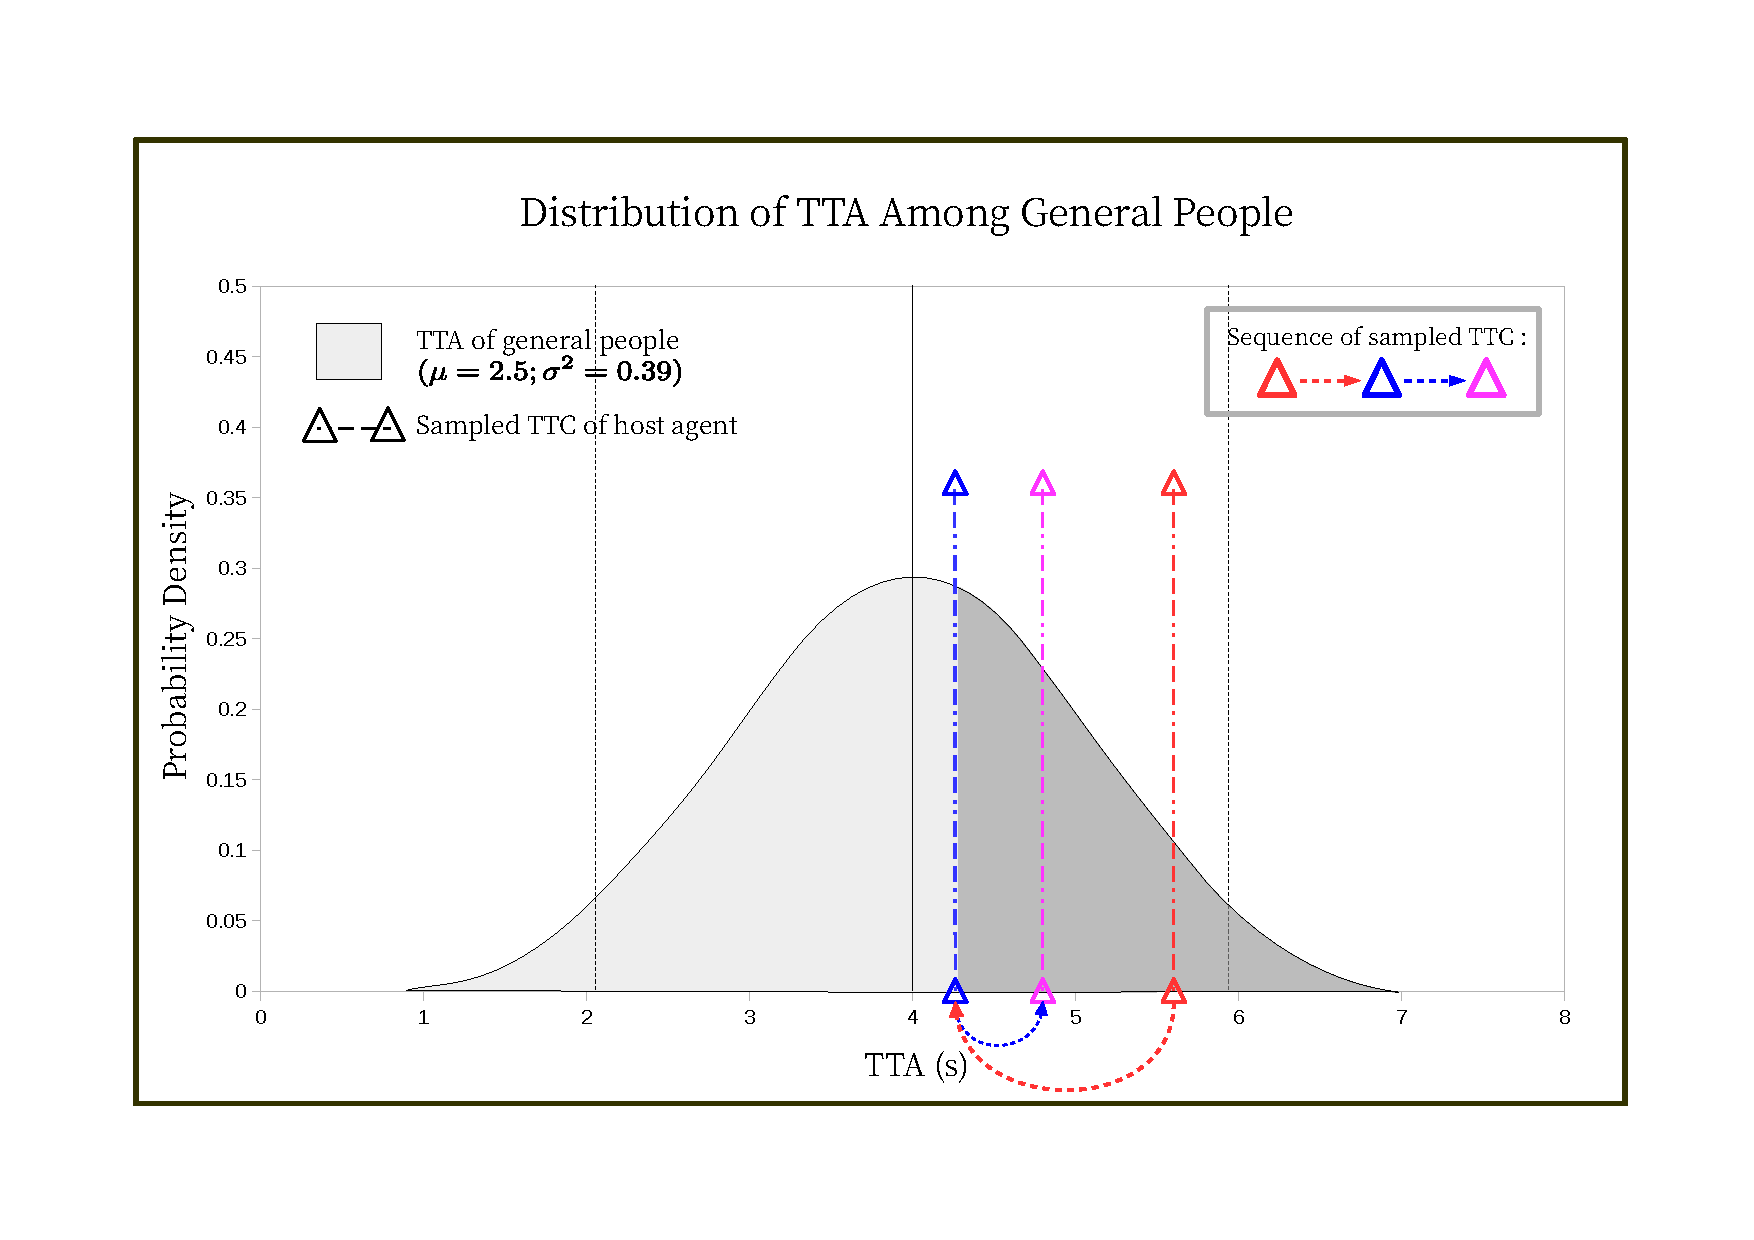
\includegraphics[scale=0.5]{TTC_probability_distribution.pdf}
\end{center}
\caption{Example of TFA distribution of general people.}
\label{fig:TTC_distribution} 
\end{figure}
 
\newpage
%%%%%%%%%%%%%%%%%%%%%%%%%%%%%%%%%%%%%%%%%%%%%%%%%%%%%
%%%%      SUBSECTION SUBSECTION SUBSECTION       %%%%   
%%%%%%%%%%%%%%%%%%%%%%%%%%%%%%%%%%%%%%%%%%%%%%%%%%%%%

\subsection{Mathematical Models of the Probability of Yielding}
\label{subsec:MathModel}

In what follows, we break down the process of braking into several parts when a driver perceives a potential danger, and formulate each part to find the TFA distribution for all drivers. Fig. \ref{fig:TTC_brake_comb} shows a vehicle at location $P_A$ cruising at a velocity $v_i$ toward the node on the right. The driver applied the brake when vehicle moves to $P_B$, and the vehicle fully stopped at $P_C$ with a safe margin $R_{\mathrm{min},i}$ to the node. The overall braking distance is $R_i$. The vehicle travels an additional distance $v_i\tau$ where $\tau$ is the reaction time from the driver decided to brake to the brake engaged. The distance to the node $d_{\mathrm{node},i, t}$ is a function of time as vehicle moves. When a driver decides to yield, $d_{\mathrm{node},i, t}$ will be the distance required to fully stopped without collision, defined as the \textit{distance left before action} in Fig.~\ref{fig:TTC_brake_comb} .

% \begin{figure}[htbp!]
% \begin{center}
%     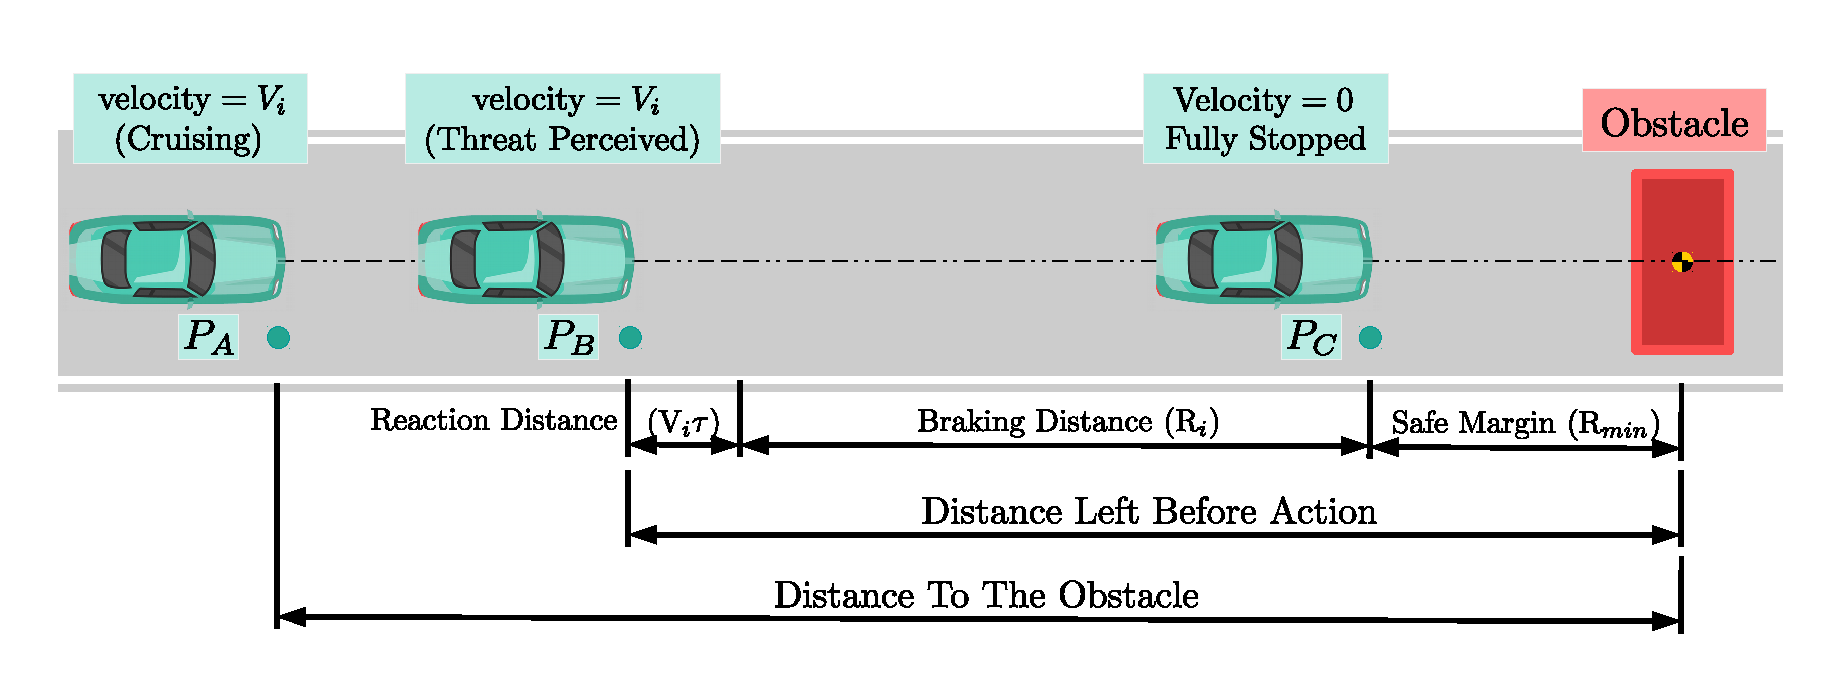
\includegraphics[scale=0.45]{TFA_TTC_model.pdf}
% \end{center}
% \caption{Decomposing the distance left before action (apply the brake).}
% \label{fig:TTC_brake_comb} 
% \label{fig:TFA_model} 
% \end{figure}

\begin{equation}
\text{Distance Left Before Braking} = R_i+v_i\tau+R_{\mathrm{min},i}
\label{eq:TFA_distance}
\end{equation}

\begin{equation}
R_{i} = \frac{v_i^2}{2a_{\mathrm{dec},i}}
\label{eq:R_i}
\end{equation}

\subsubsection{The distance left before action}
The distance left before action is the sum of the reaction distance, the braking distance and the safe margin as shown in Eqn.(\ref{eq:TFA_distance}). The reaction distance $v_i \tau$ consider both the perception-reaction of a driver and the system actuation delay, and the reaction time $\tau$ in this work is considered as a constant biological trait under various vehicle speeds. The braking distance is shown in Eqn.(\ref{eq:R_i}), where $a_{\mathrm{dec},i}$ is the deceleration during the brake by assuming constant deceleration throughout the entire braking process. The last parameter, safe margin, is denoted as $R_{\mathrm{min},i}$, which stands for the safe distance that the driver left after the vehicle is fully stopped. For the sake of making data extraction easier, the $R_{\mathrm{min},i}$ is defined as distance from the center of one vehicle to another. Using the definition of TFA and Eqn.(\ref{eq:TTC_dv}), we divided the distance left before braking (as in Eqn.(\ref{eq:TFA_distance})) by the speed of the vehicle ${v_i}$, TFA can then be estimated using Eqn.(\ref{eq:TFA_est}).

\begin{equation}
\text{TFA}_{\mathrm{est},i} = \frac{R_i+v_i\tau+R_{\mathrm{min},i}}{v_i} 
\label{eq:TFA_est}
\end{equation}

In Eqn.(\ref{eq:RMIN_Linear}) and Eqn.(\ref{eq:ADEC_Linear}), $R_{\mathrm{min},i}$ and $a_{\mathrm{dec},i}$ are treated as functions of speed and are linearly formulated as Eqn, which reflect situations with different severity levels. For example, drivers might have more aggressive actions when being at lower speed (e.g. smaller $R_{\mathrm{min},i}$ for closer distance to the other vehicle after stopped) , since they believe everything is under control (i.e. the severity of the collision is low). While at high speed, drivers tend to act more conservatively (e.g. larger $R_{\mathrm{min},i}$ to keep a larger "safer margin") to avoid serious collisions. 
 
\begin{equation}
R_{\mathrm{min},i} = {C1}_{\mathrm{Rmin},i} v_i + {C2}_{\mathrm{Rmin},i}
\label{eq:RMIN_Linear}
\end{equation}

\begin{equation}
a_{\mathrm{dec},i} = {C1}_{\mathrm{adec},i} v_i + {C2}_{\mathrm{adec},i}
\label{eq:ADEC_Linear}
\end{equation}

\noindent where Safe Margin Coefficient (${C1}_{\mathrm{Rmin},i}$), Safe Margin Constant (${C2}_{\mathrm{Rmin},i}$), Deceleration Coefficient (${C1}_{\mathrm{adec},i}$), and Deceleration Constant (${C2}_{\mathrm{adec},i}$) standing for the coefficients and constants of the linear equation of $R_{\mathrm{min},i}$ and $a_{\mathrm{dec},i}$.

The proposed Probability of Yielding (POY) at time $t$, denoted as $P_{\mathrm{yield}, i,t}$, is shown in Eqn.(\ref{eq:POY}).  

\begin{equation}
    P_{\mathrm{yield}, i,t} = \Bigr(1-\Phi_{\mu, \sigma^{2},i}\big({\mathrm{min TTC}}_{i,t}\big)\Bigl)
\label{eq:POY}
\end{equation}

\noindent  where ${\mathrm{minTTC}}_{i,t}$ is the minimum TTC during the process as we discussed in Fig.~\ref{fig:TTC_TFA_indicator} and Fig.~\ref{fig:TTC_distribution}, and $\Phi_{\mu, \sigma^{2},i}$ is the CDF of the TFA distribution, indicated by dark grey area in Fig. \ref{fig:TTC_distribution}. Once we have the TFA distribution and the minimum TTC of the surrounding vehicle, we are able to calculate its POY using Eqn.(\ref{eq:POY}). However, before that, some adjustment terms are required to allow the POY estimation covers all possible situations.

\subsubsection{Adjustments for acceleration}
Drivers might determine to accelerate to avoid a potential collusion instead of braking. If vehicle accelerations are not taken into account, some intentions might be misunderstood. For example, a vehicle moving toward intersection with constant speed or even little acceleration would be interpreted as having the intention to brake if only the minimum TTC is considered. Let us now look at Fig.~\ref{fig:TTC_acc}, from the top to the bottom are the velocity, the distance to the node, and the TTC of surrounding vehicle respectively. Fig.~\ref{fig:TTC_acc} shows a constant acceleration scenario, as the vehicle speed up, the displacement to the node drops in a parabolic curve since the vehicle is moving closer. The resulting TTC curve, defined by Eqn.(\ref{eq:TTC_dv}), is also decreasing and even goes beneath 0. In the cases like this one, the POY using merely the integral from the TFA distribution, as in Fig.~\ref{fig:TTC_distribution}, would causing the increase of the POY as the TTC keeps decreasing.

\begin{figure}[htbp!]
\begin{center}
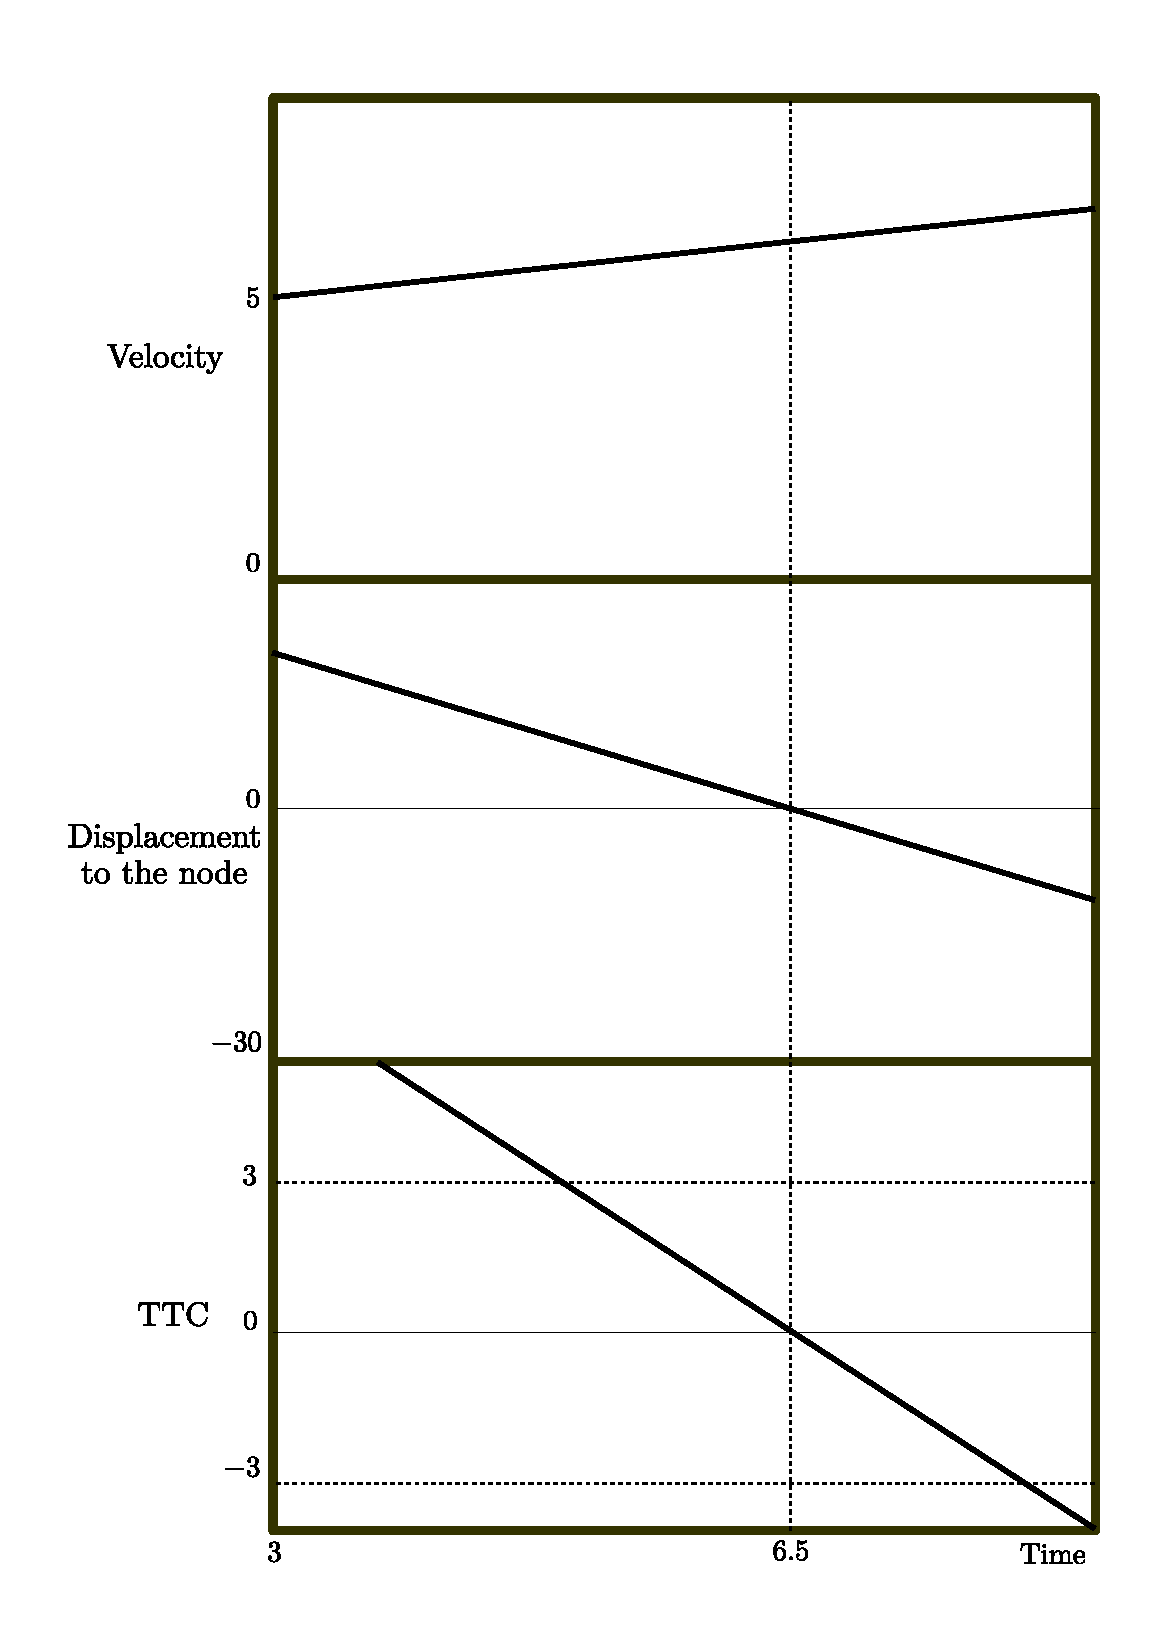
\includegraphics[scale=0.6]{TTC_change_when_accelerating.pdf}
\end{center}
\caption{History of TTC as the surrounding vehicle accelerating through the node.}
\label{fig:TTC_acc} 
\end{figure}

We consider an acceleration related term $A_{i,t}$ (Eq.(\ref{eq:alpha_cap})) as the adjusted mean value of the TFA distribution in Eq.(\ref{eq:d_node}). $\alpha_{i,t}$ defines how strongly the acceleration term affects the mean value of the TFA distribution, and the $\beta_{i,t}$ is used to prevent some disturbance introduced by sensor error or other noise.To avoid the consequences for neglecting the accelerations, the adjustments term is defined by following equations.

\begin{equation}
\mu_{i,t} = {\mathrm{TFA}}_{\mathrm{est}, i,t} + A_{i,t}
\label{eq:d_node}
\end{equation}

\begin{equation}
    A_{i,t} = 
    \begin{cases} 
      \alpha_{i,t} &~~\text{if}~~ \lvert \alpha_{i,t} - \alpha_{t-1,i}  \rvert < 1.67 \cdot \sigma_{est}\\
      \frac{\alpha_{i,t}}{\lvert \alpha_{i,t} \rvert} \cdot 1.67 \cdot \sigma_{est} &~~\text{otherwise}
    \end{cases}
\label{eq:alpha_cap}
\end{equation}

\begin{equation}
    \alpha_{i,t} = 
    \begin{cases} 
      \beta_{i,t} \cdot \ln \left ( ~ \left( ~ \lvert {\mathrm{TTC}'}_{i,t}  \rvert + 1 ~\right) \cdot e~ \right) &~~\text{if}~~ {\mathrm{TTC}'}_{i,t} > -1\\
      - \beta_{i,t} \cdot \ln \left ( ~ \left( \lvert {\mathrm{TTC}'}_{i,t}  \rvert + 1 \right) \cdot e~ \right) &~~\text{if}~~ {\mathrm{TTC}'}_{i,t} < -1 \\
      \alpha_{t-1,i} &~~\text{otherwise}
    \end{cases}
\label{eq:alpha}
\end{equation}

\begin{equation}
    \beta_{i,t} = 
     \max ~ \big( ~ \lvert {\mathrm{min TTC}}_{i,t} - \mathrm{TFA}_{\mathrm{est}, i,t} \rvert, ~ \sigma_{\mathrm{est}} ~ \big)
\label{eq:beta}
\end{equation}

The ${\mathrm{TTC}'}_{i}$ (the first order derivative of TTC) in Eqn.(\ref{eq:d_node}) is used to take acceleration, displacement and speed into account for the POY adjustment. It is obtained from the derivative of Eqn.(\ref{eq:TTC_dv}) under the assumption of constant acceleration.

\begin{equation}
\mathrm{TTC}'_{i} = \frac{d}{dt}\frac{d_{\mathrm{node},i}}{v_{i}} = -1 -a \cdot d_{\mathrm{node},i} \cdot v_{i}^{-2}
\label{eq:TTC'}
\end{equation}

We can see in Eqn.(\ref{eq:TTC'}) that the $\mathrm{TTC}'_i$ equals -1 when the acceleration is 0, greater than -1 when the subject vehicle is decelerating, and less than -1 when accelerating. If we bring these into to Eqn.(\ref{eq:alpha_cap}), we find that the mean value of the TFA distribution is increased when $A_{i, t}$ is positive (the surrounding vehicle is decelerating), which means the resulting POY will increase under the same TTC, due to the larger integral of that area under TFA distribution, as illustrated in Fig.~\ref{fig:TFA_weighting_comb}. In this figure, the current TTC equals the mean of the TFA distribution so the resulting POY is 0.5, indicated by the lighter grey area. However, since the vehicle is decelerating, the mean value of the TFA distribution is adjusted according to Eqn.(\ref{eq:alpha}). The POY, which is the area under the TFA distribution and right to the current TTC, becomes 0.97, shown as the darker grey area in Fig.~\ref{fig:TFA_weighting_comb}.

\begin{figure}[htbp!]
\begin{center}
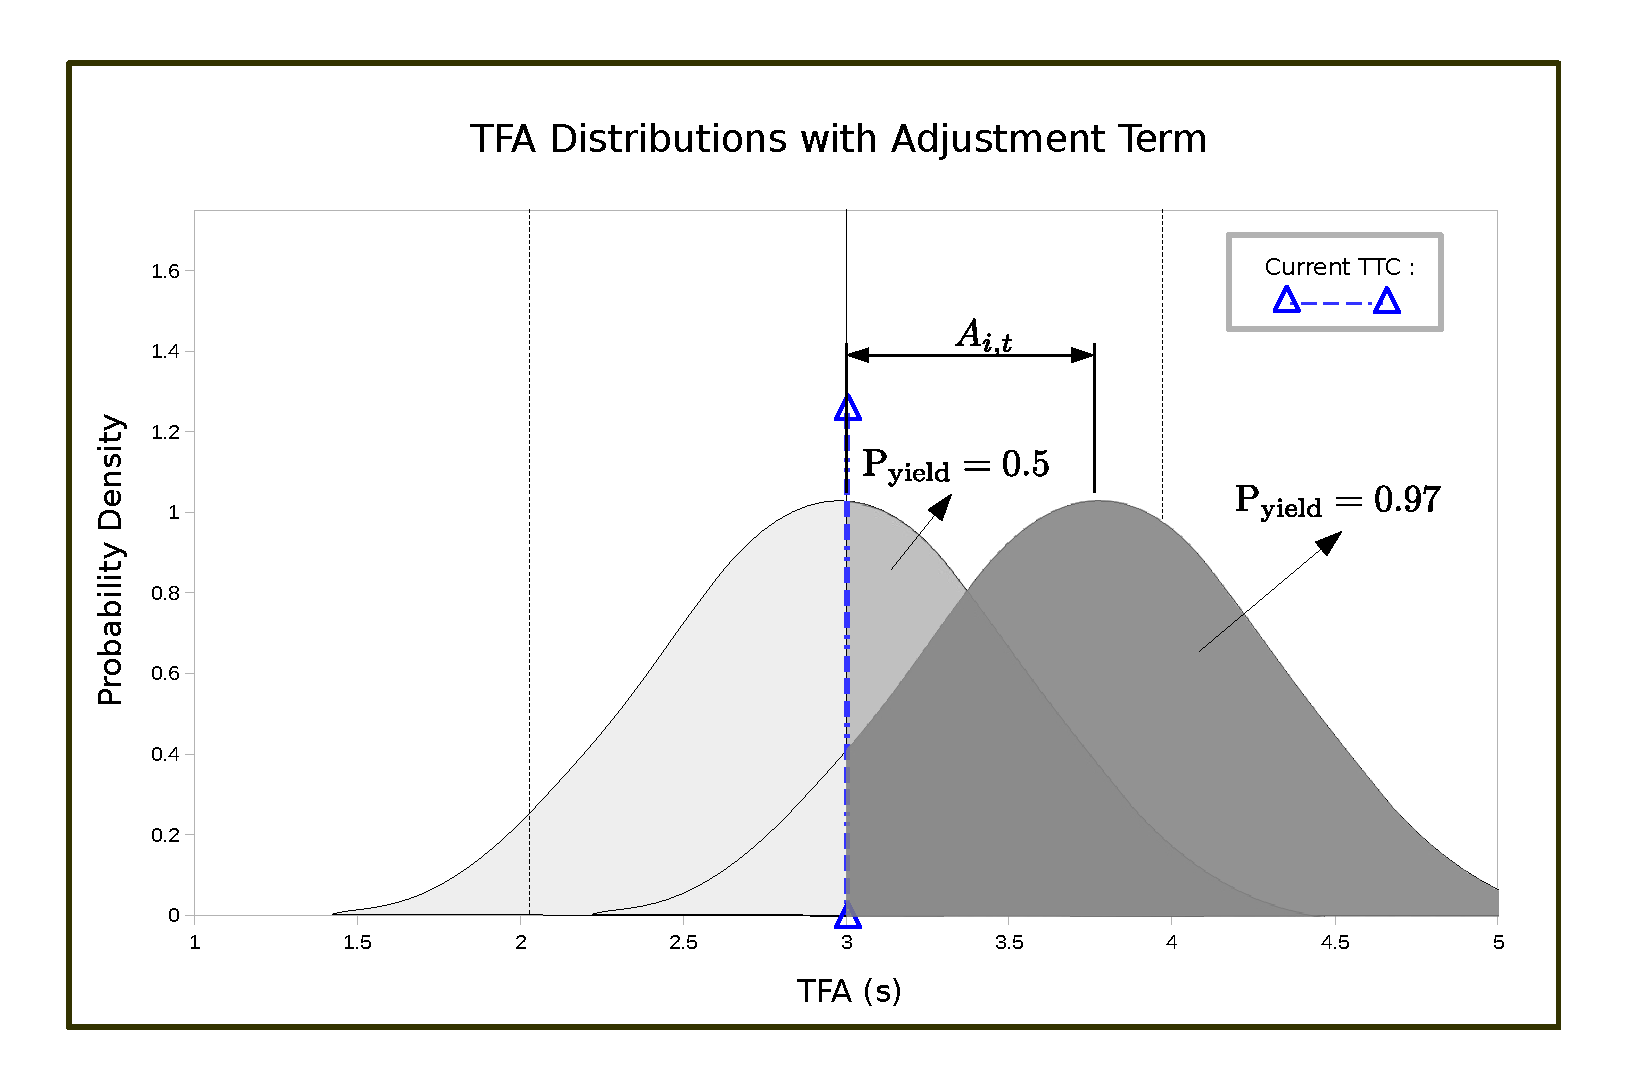
\includegraphics[scale=0.5]{TFA_weighting_comb.pdf}
\end{center}
\caption{The effect of the weighting parameter $A_{i,t}$ on TFA distribution.}
\label{fig:TFA_weighting_comb} 
\end{figure}

% \begin{figure}[htbp!]
% \begin{center}
% 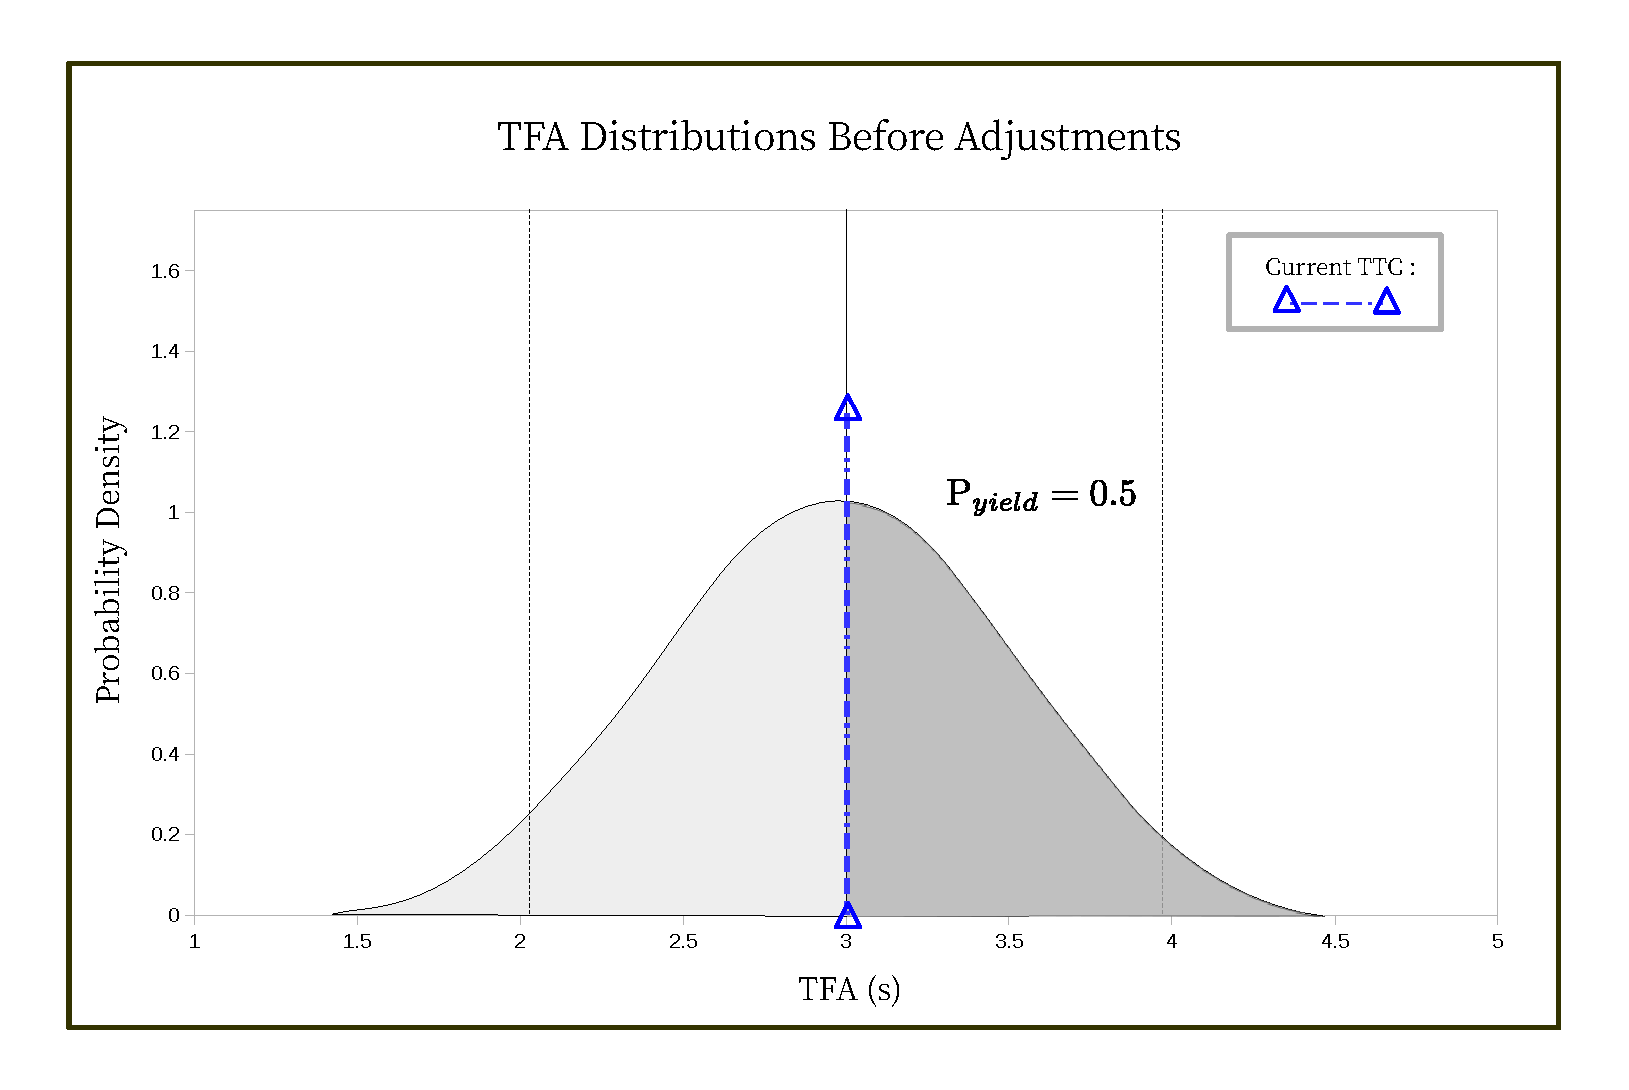
\includegraphics[scale=0.4]{TFA_weighting_before.pdf}
% \end{center}
% \caption{The probability before the weighting parameter $A_t$ is 0.5 .}
% \label{fig:TFA_weighting_before} 
% \end{figure}

% \begin{figure}[htbp!]
% \begin{center}
% 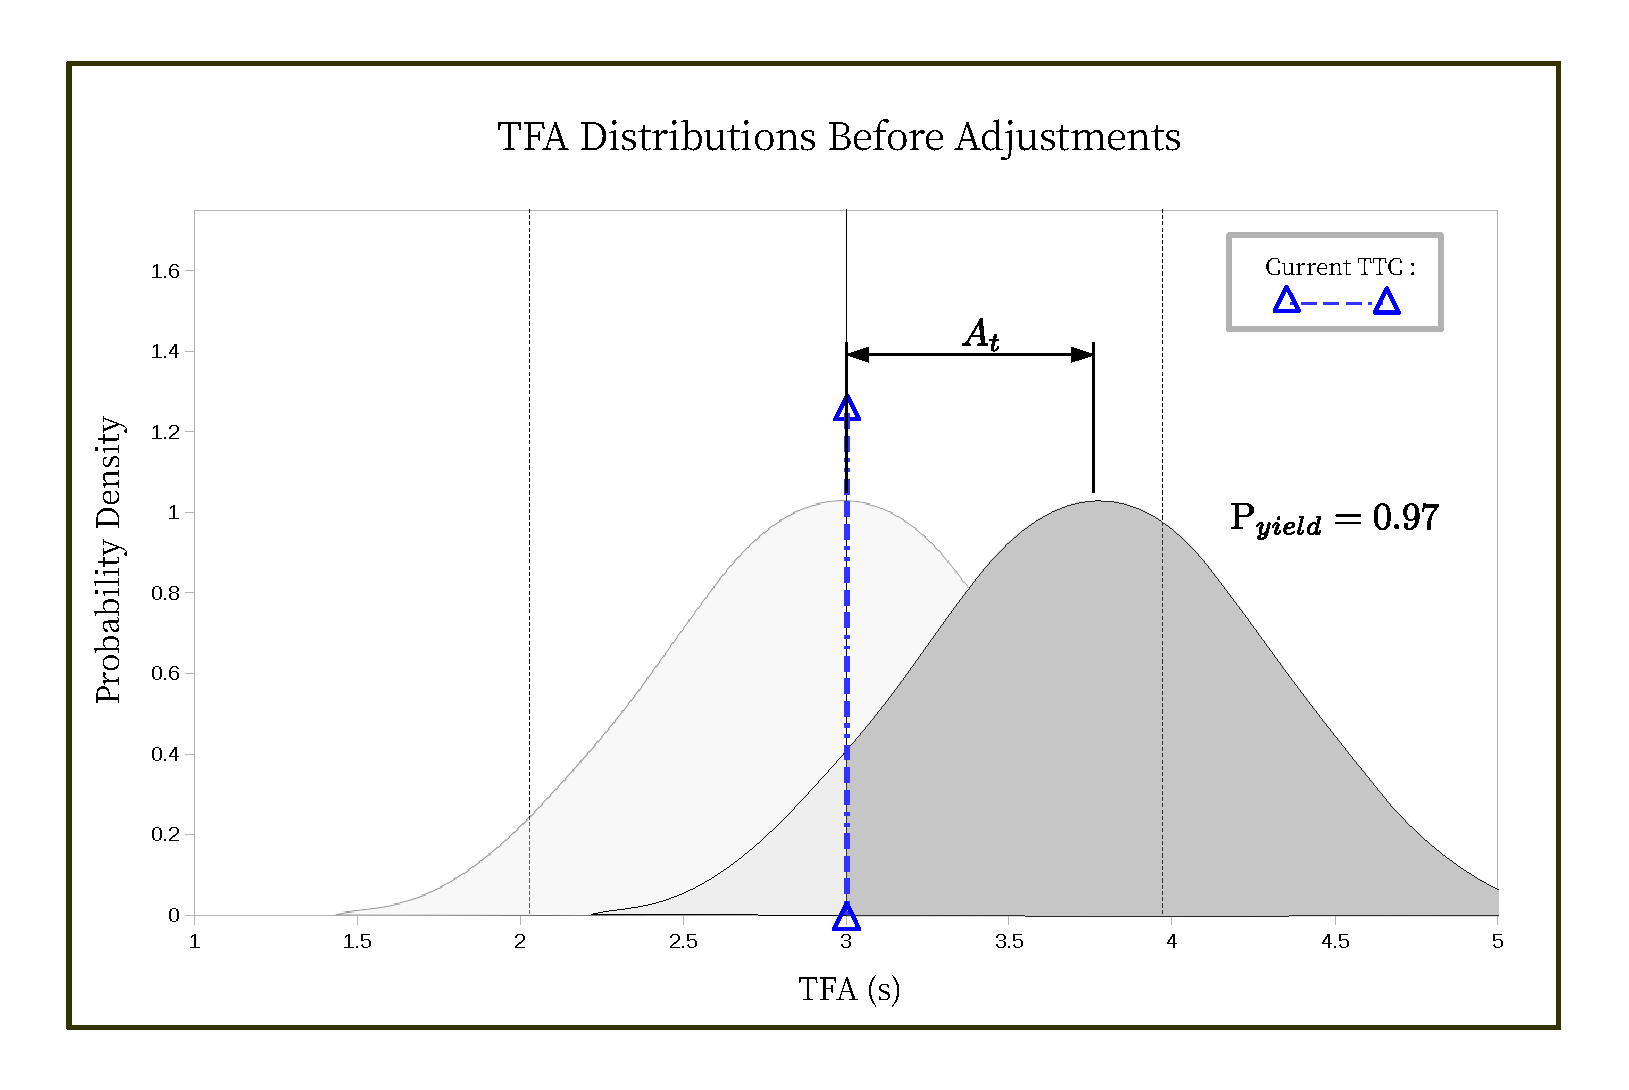
\includegraphics[scale=0.4]{TFA_weighting_after.pdf}
% \end{center}
% \caption{The probability after the weighting parameter $A_t$ is 0.97 .}
% \label{fig:TFA_weighting_after} 
% \end{figure}


In Eqn.(\ref{eq:alpha}), the magnitude of $\alpha_t$ is adjusted depending on the greater one between $\lvert {\mathrm{min TTC}}_{t} - \mathrm{TFA}_{\mathrm{est}, t} \rvert $ and $ \sigma_{\mathrm{est}, t}$ (as shown in Eqn.(\ref{eq:beta})), which allows the proposed model to have more immediate response to the situation at the moment. Jagged POY curve might be shown, however, if the response is "too immediate", the maximum value of $A_{i,t}$ is set to 1.67 standard deviation to suppress the value and prevent the POY from rising or dropping too rapidly.

% \subsubsection{TFA Distribution Estimation}

\subsubsection{TFA Distribution Parameters Estimation via Experiments}

Parameters for TFA distributions are determined via a series of simulated crossroad experiments in this study. In our experiments, participants are asked to drive toward a static vehicle with constant speed and apply the brake when they believe that the collision will happen. The probability plot in Fig.~\ref{fig:TFA_distr_combined} shows that the probability plot of the results matches a Gaussian distribution.  Therefore for the remaining of the article, we assume that all TFA are Gaussian distributed , with ${\mathrm{TFA}}_{\mathrm{est}}$ as the estimated mean value and $\sigma_{\mathrm{est}}$ as the standard deviation with the value 0.35. 
  

% \begin{equation}
% \text{TFA} \sim N(\text{TFA}_{est},\,\sigma_{est}^{2}).
% \label{eq:TFA_distribution}
% \end{equation}
\begin{figure}[htbp!]
    \centering
    \subfloat[TFA distribution for all participants are displayed in histogram. The solid curve is the results approximated by Normal distribution ($\mu = 2.37, \sigma = 0.35, N = 197$). ]
    {
    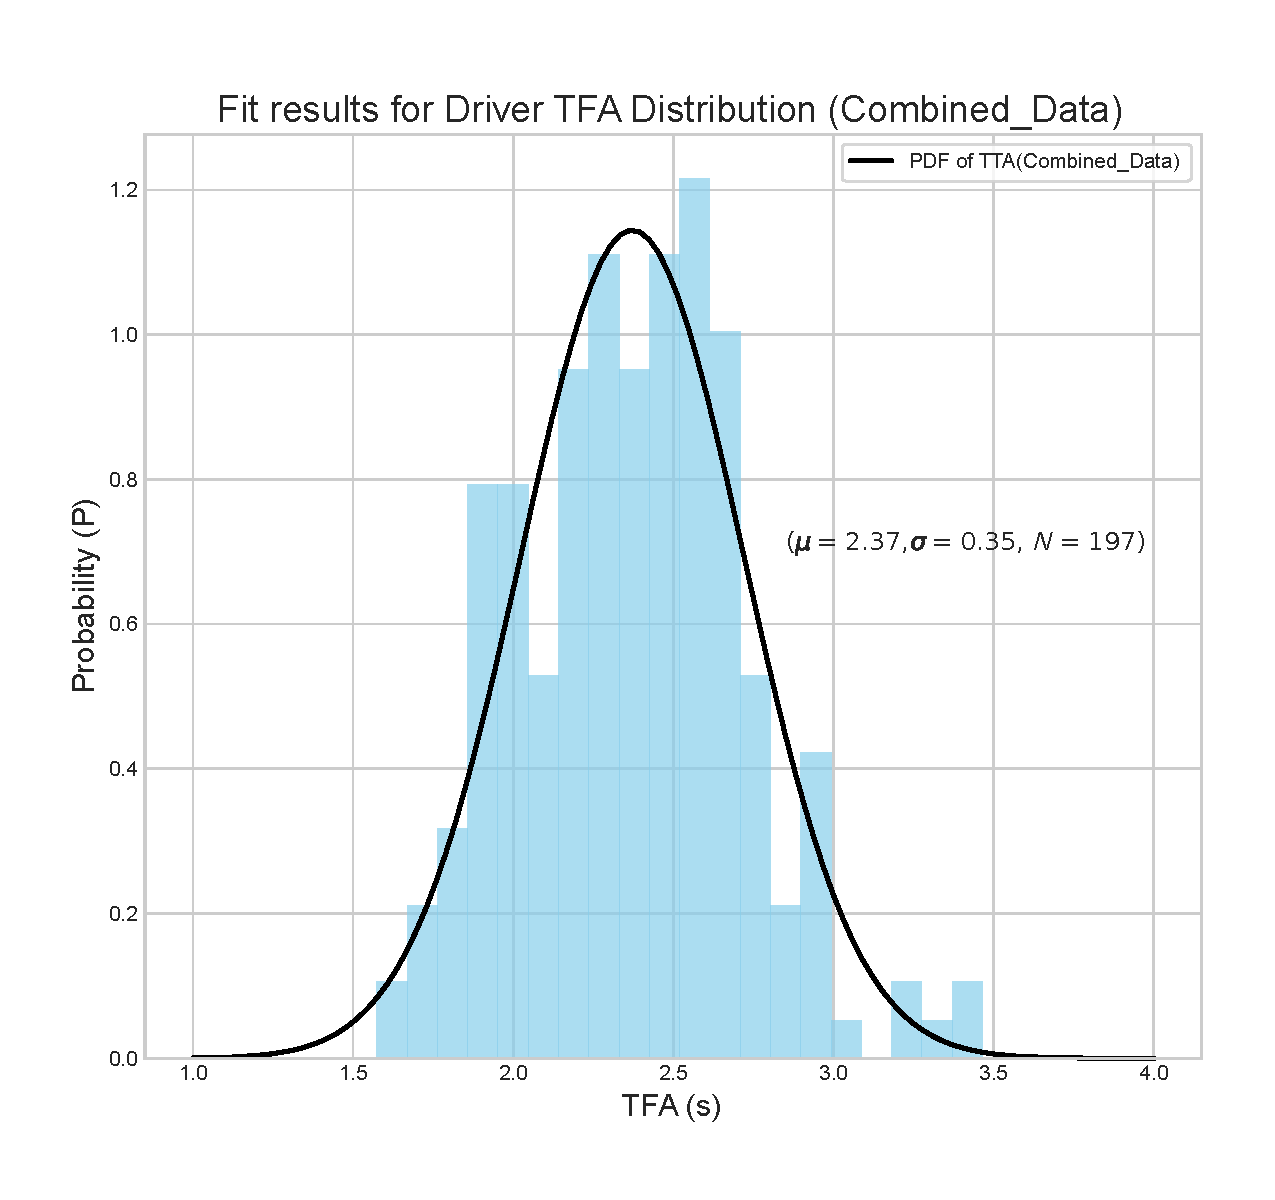
\includegraphics[width=0.47\textwidth]{fit_TFAdist_comb.pdf}
    \label{fig:TFAdist_comb}
    }\hfill
    \subfloat[Quantile-Quantile plot for the TFA distribution of the combined data against normal distribution.]
    {
    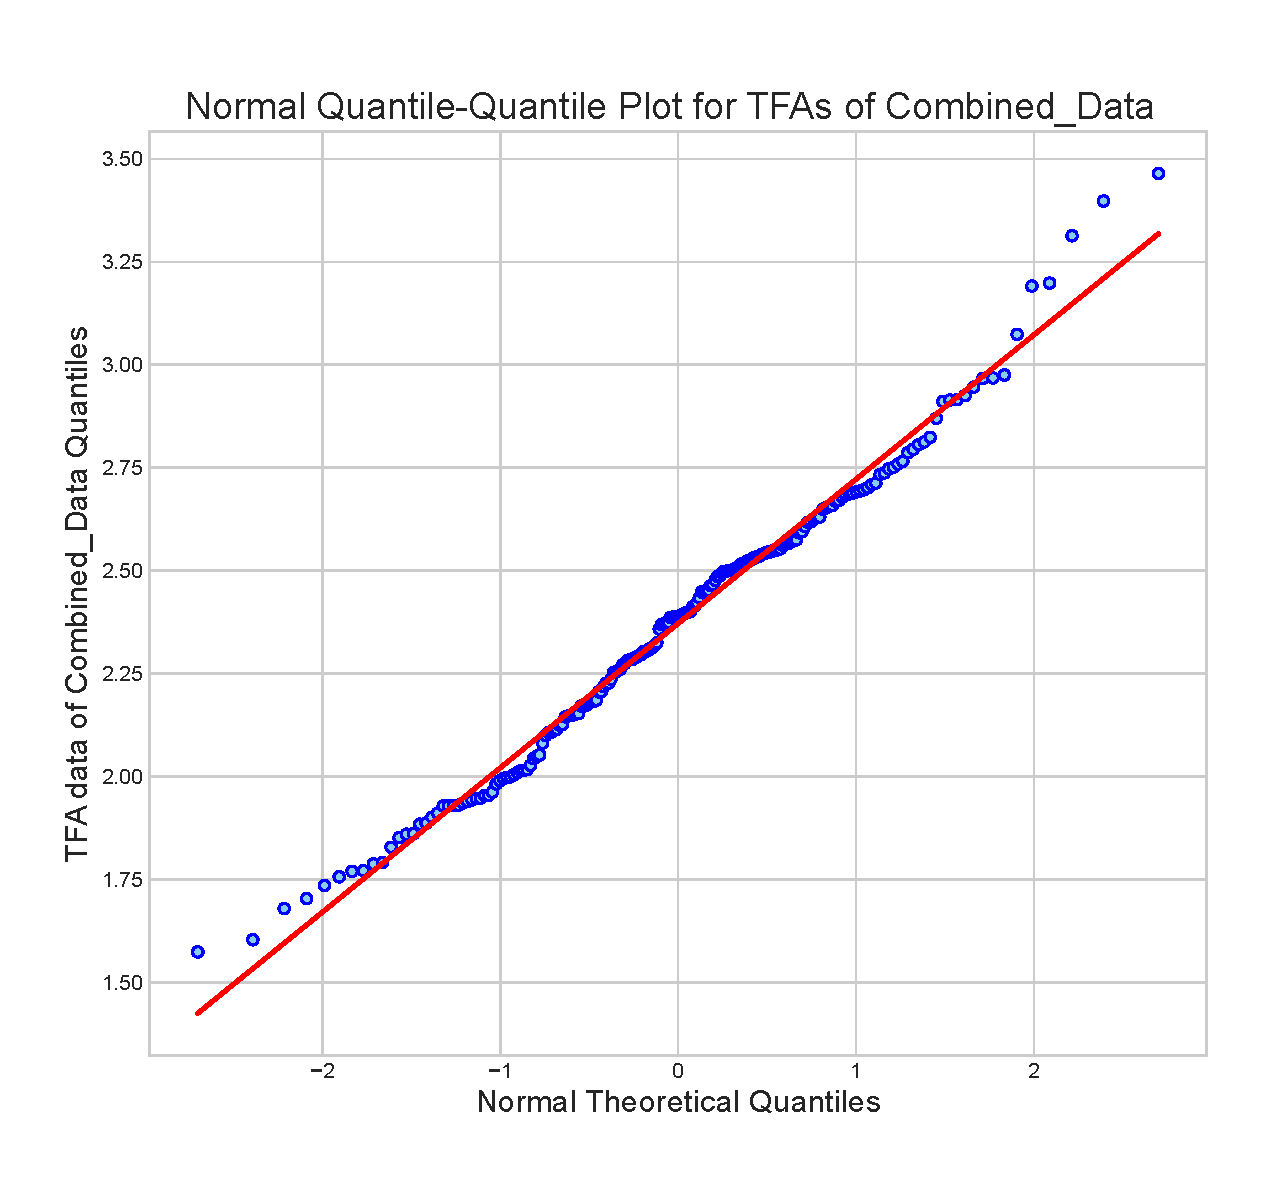
\includegraphics[width=0.47\textwidth]{fit_TFAdist_comb_qqp.pdf}
    \label{fig:TFAdist_comb_qqp}
    }\hfill
    \caption{TFA distribution of combined data fitted normally, with Quantile-Quantile plot showing its relationship with normal distribution. }
\label{fig:TFA_distr_combined} 
\end{figure}

% \noindent and the value of the variance $\sigma^2$ is defined as 

% \begin{equation}
% \sigma_{est} = \gamma \cdot \text{TFA}_{est}
% \label{eq:TFA_distribution}
% \end{equation}

% \noindent where $\gamma$ is the coefficient for standard deviation, which is obtained from the ratio of $\mu$ and $\sigma$ obtained from the approximated normal distribution of TFA. 

From the experiments, we also shown that $R_{\mathrm{min}}$ and $a_{\mathrm{dec}}$ are functions of $v_i$ and can be approximated by linear equation, which are formulated in Eqn.(\ref{eq:RMIN_Linear}) and Eqn.(\ref{eq:ADEC_Linear}). Fig.~\ref{fig:CombRMINDifSpeed} and \ref{fig:CombADECDifSpeed} shows the results of $R_{\mathrm{min}}$ and $a_{\mathrm{dec}}$ under various velocity in our experiments. We can see that the $R_{\mathrm{min}}$ does get higher linearly as the velocity rises, which is the same as predicted. Same trends happen to $a_{\mathrm{dec}}$ as the velocity ascends, which suggests that drivers brake slowly at low velocity and rapidly at high velocity. This result is also reasonable, since the situation tends to be more urgent when the velocity is high. Now we have all the elements needed, the required TFA distribution under different speed can now be estimated using ${\mathrm{TFA}}_{\mathrm{est}}$. Parameters used in the proposed TFA distribution estimation are listed in Table~\ref{table:parameters}. 


\begin{figure}[htbp!]
\begin{center}
\makebox[0pt]{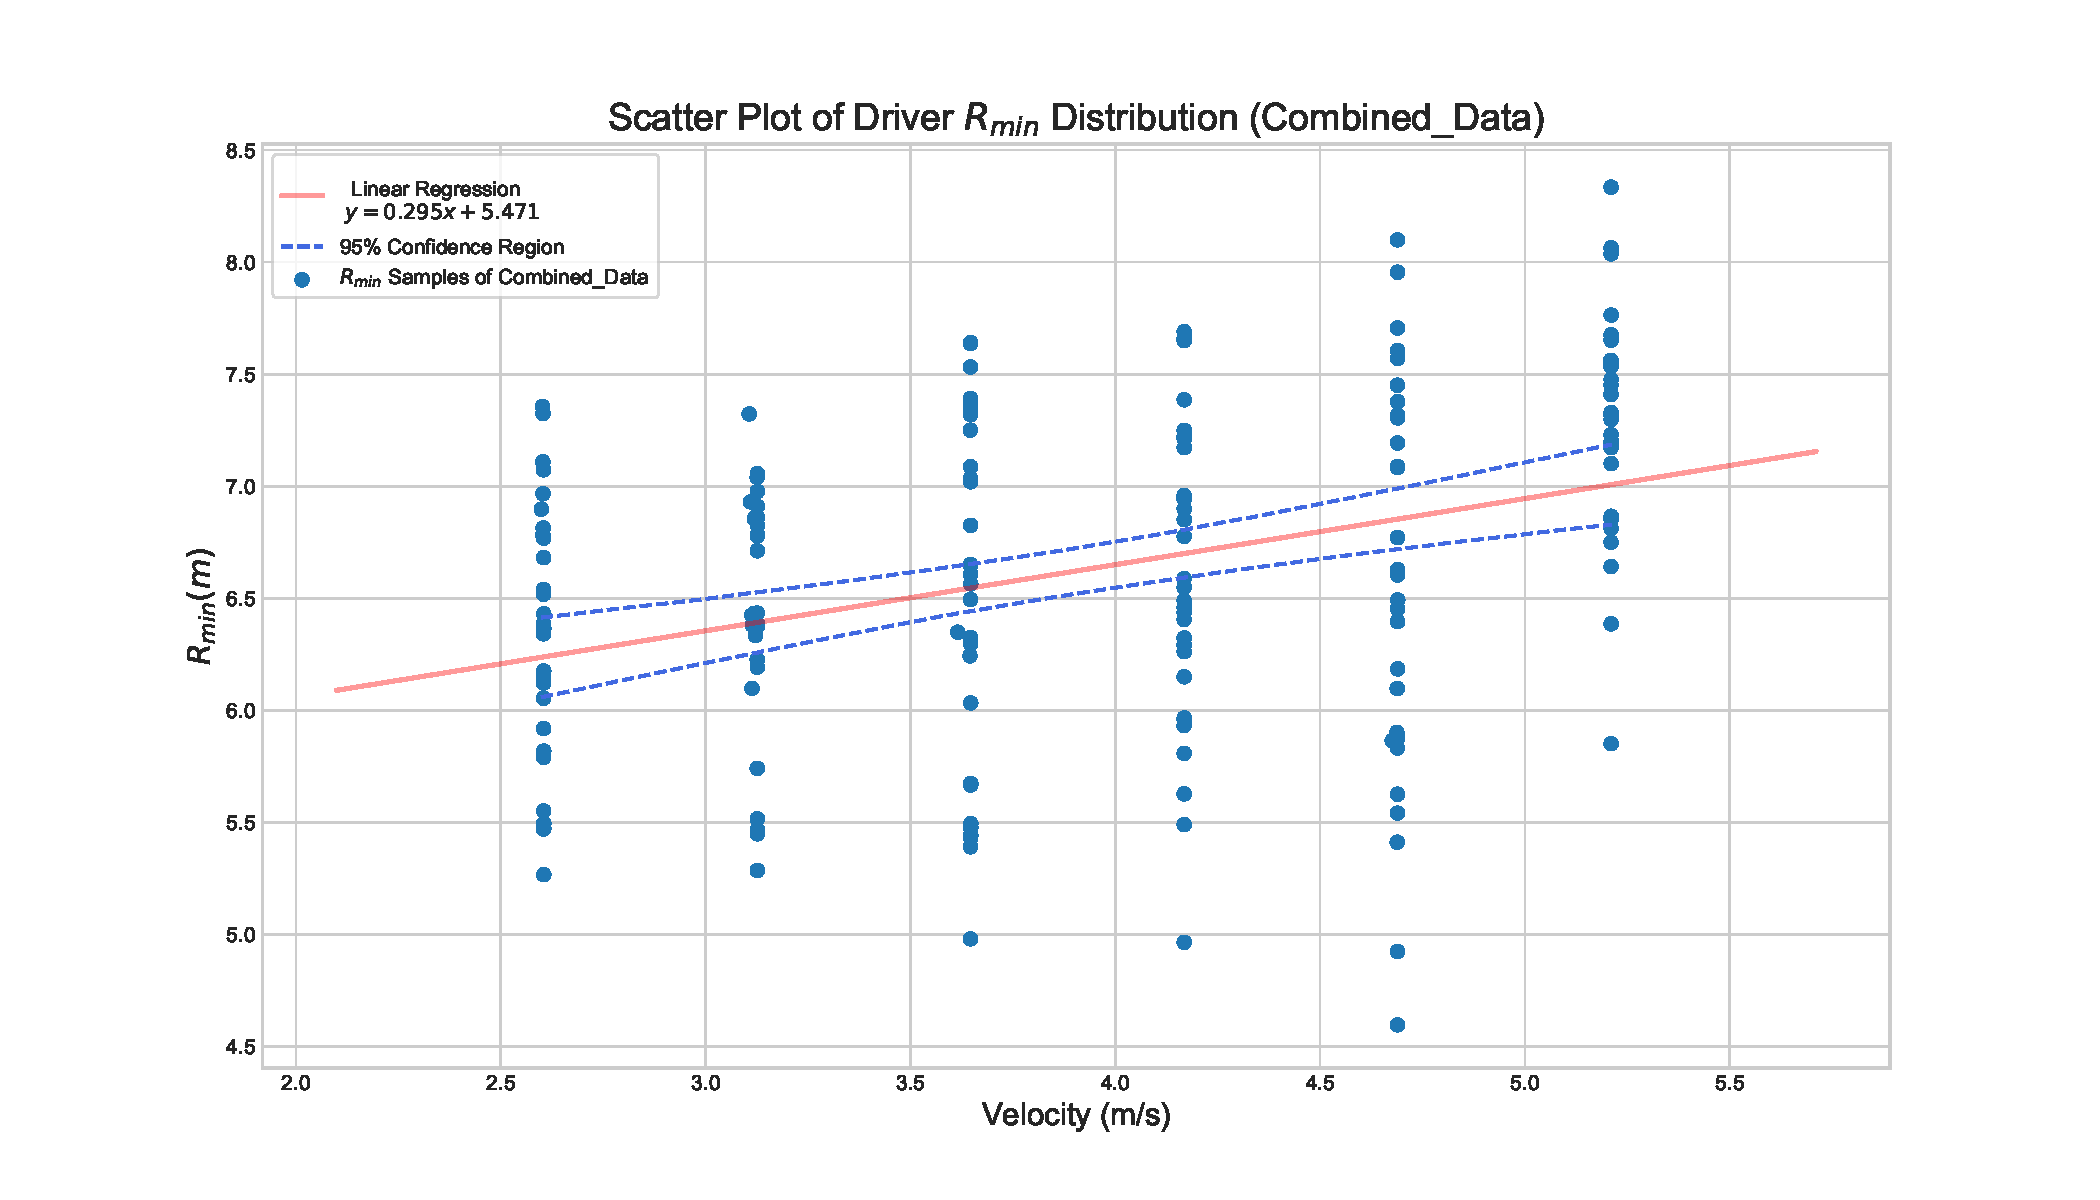
\includegraphics[width=0.7\paperwidth]{Combined_Data_R_MIN_polyfit.pdf}}
\end{center}
\caption{The $R_{\mathrm{min}}$ scatter plot of combined data under various velocities.}
\label{fig:CombRMINDifSpeed} 
\end{figure}

\begin{figure}[htbp!]
\begin{center}
\makebox[0pt]{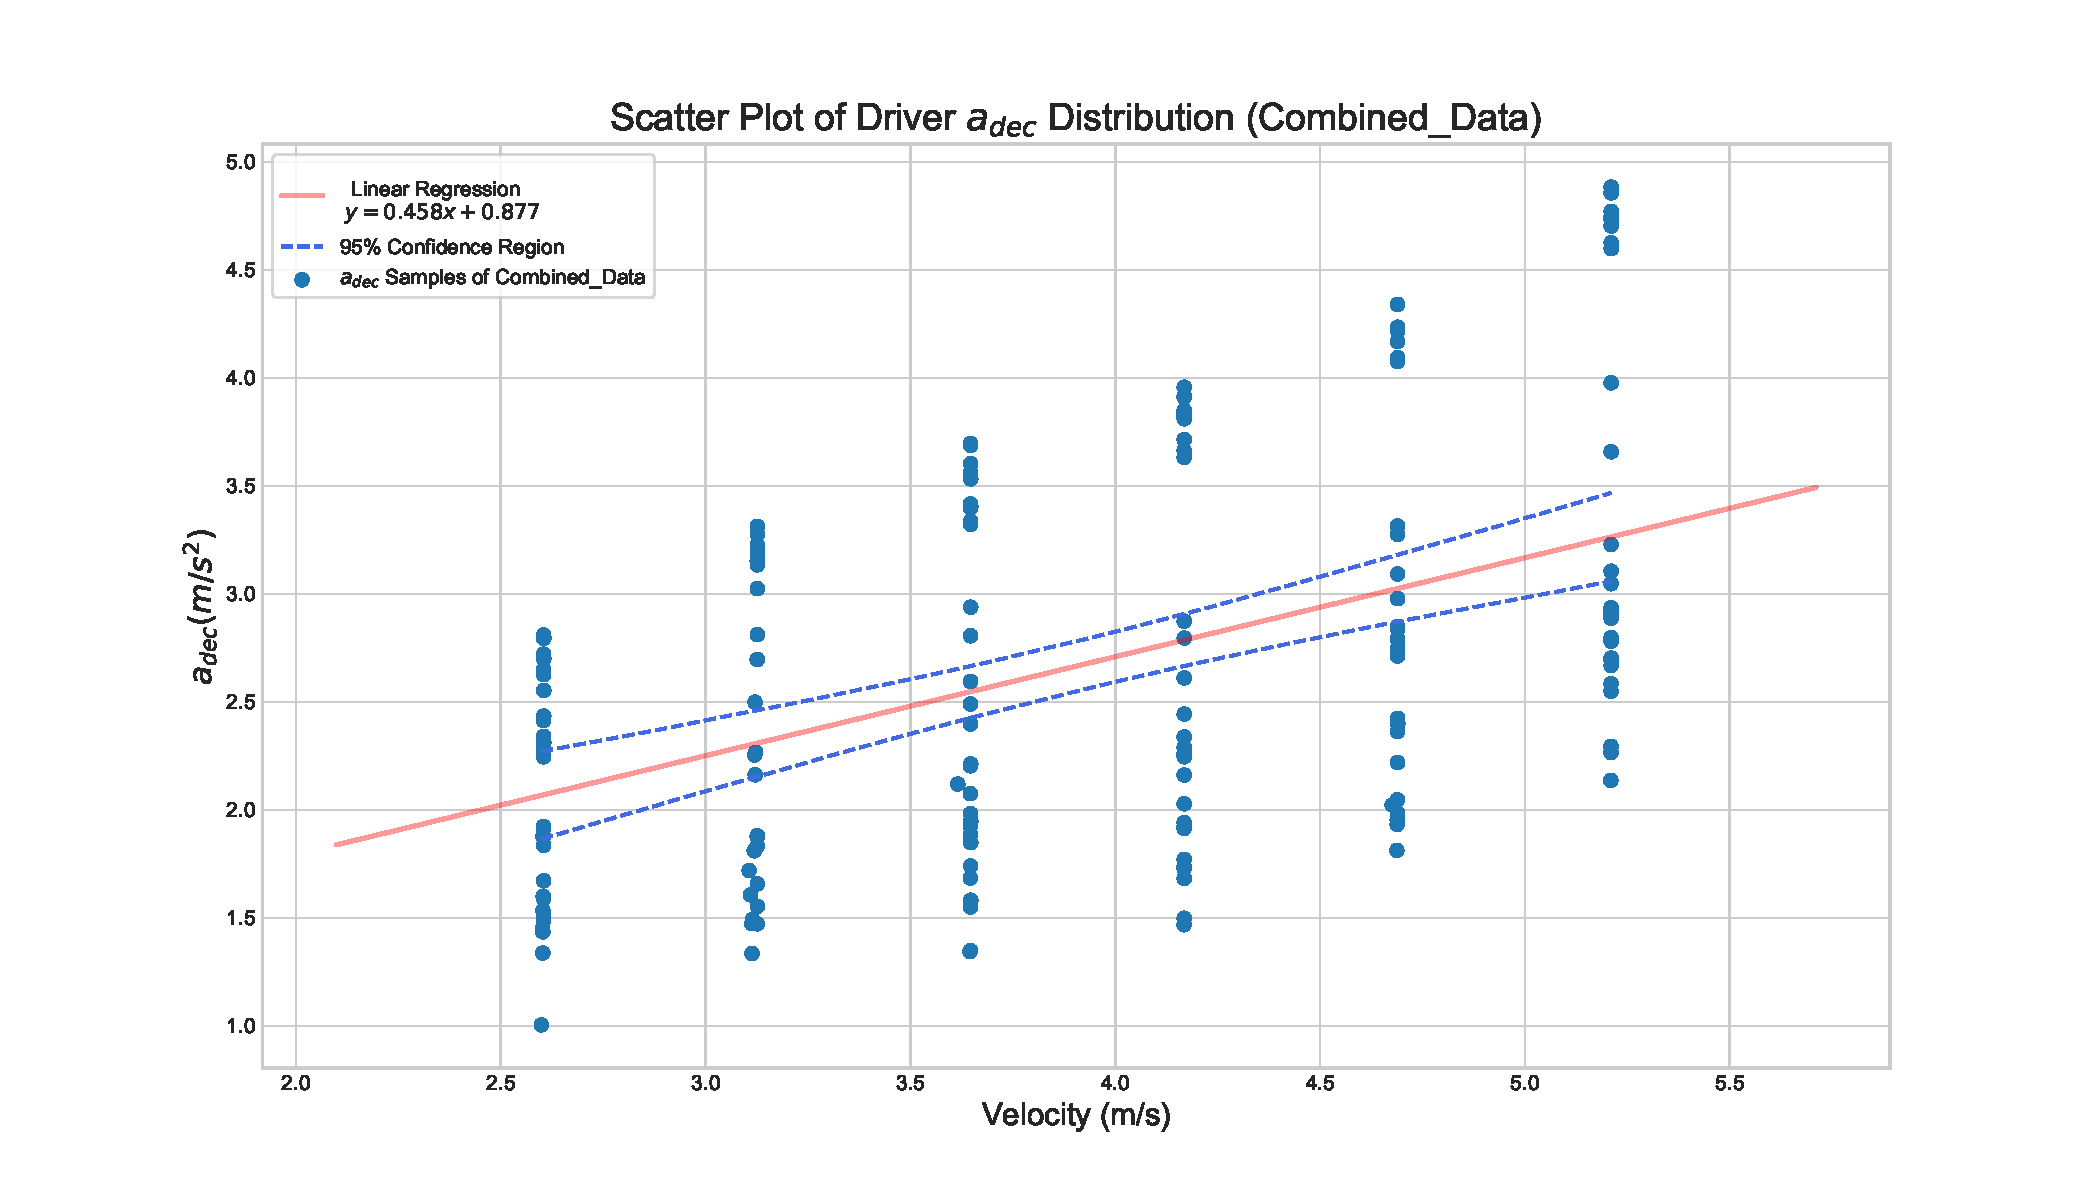
\includegraphics[width=0.7\paperwidth]{Combined_Data_A_DEC_polyfit.pdf}}
\end{center}
\caption{The $a_{\mathrm{dec}}$ scatter plot of combined data under various velocities.}
\label{fig:CombADECDifSpeed} 
\end{figure}

% \noindent where the approximated  equations for $R_{MIN}$ and $a_{dec}$ are

% \begin{equation}
% R_{min} = 0.295 v_i + 5.471
% \label{eq:RMIN_Linear}
% \end{equation}

% \begin{equation}
% a_{dec} = 0.458 v_i + 0.877
% \label{eq:ADEC_Linear}
% \end{equation}


\begin{table}[htbp]
\caption{Table for parameters used in TFA distribution model.}
\begin{center}
\label{table:parameters}
\begin{tabular}{l l l l c}
& & \\ % put some space after the caption
\hline
\textbf{Parameters} &  & & &\textbf{Values} \\
\hline
Safe Margin Coefficient (${C1}_{\mathrm{Rmin}}$)     &  &  & &  0.295  \\
Safe Margin Constant (${C2}_{\mathrm{Rmin}}$)     &  &  & &  5.471  \\
Deceleration Coefficient (${C1}_{\mathrm{adec}}$) &  &  & & 0.458  \\
Deceleration Constant (${C2}_{\mathrm{adec}}$) &  &  & & 0.877  \\
Reaction Time ($\tau$)        &  &  & & 0.6 $s$ \\
% Standard Diviation Parameter ($\gamma$)      &  &  & & 0.148  \\
\hline
\end{tabular}
\end{center}
\end{table}

We model driver decisions at the crossroad as the probability of yielding/passing. The proposed method enables autonomous vehicles to understand the intentions of other traffic participants in a mixed-fleet environment.



%%%%%%%%------------------------------%%%%%%%%%
%%%%%%%%-----------SUBSECTION---------%%%%%%%%%
%%%%%%%%------------------------------%%%%%%%%%

\subsection{Driver Intentions Prediction with Probability of Yielding}
\label{subsec:ValidatePOY}


\begin{figure}[htbp!]
\begin{center}
\makebox[0pt]{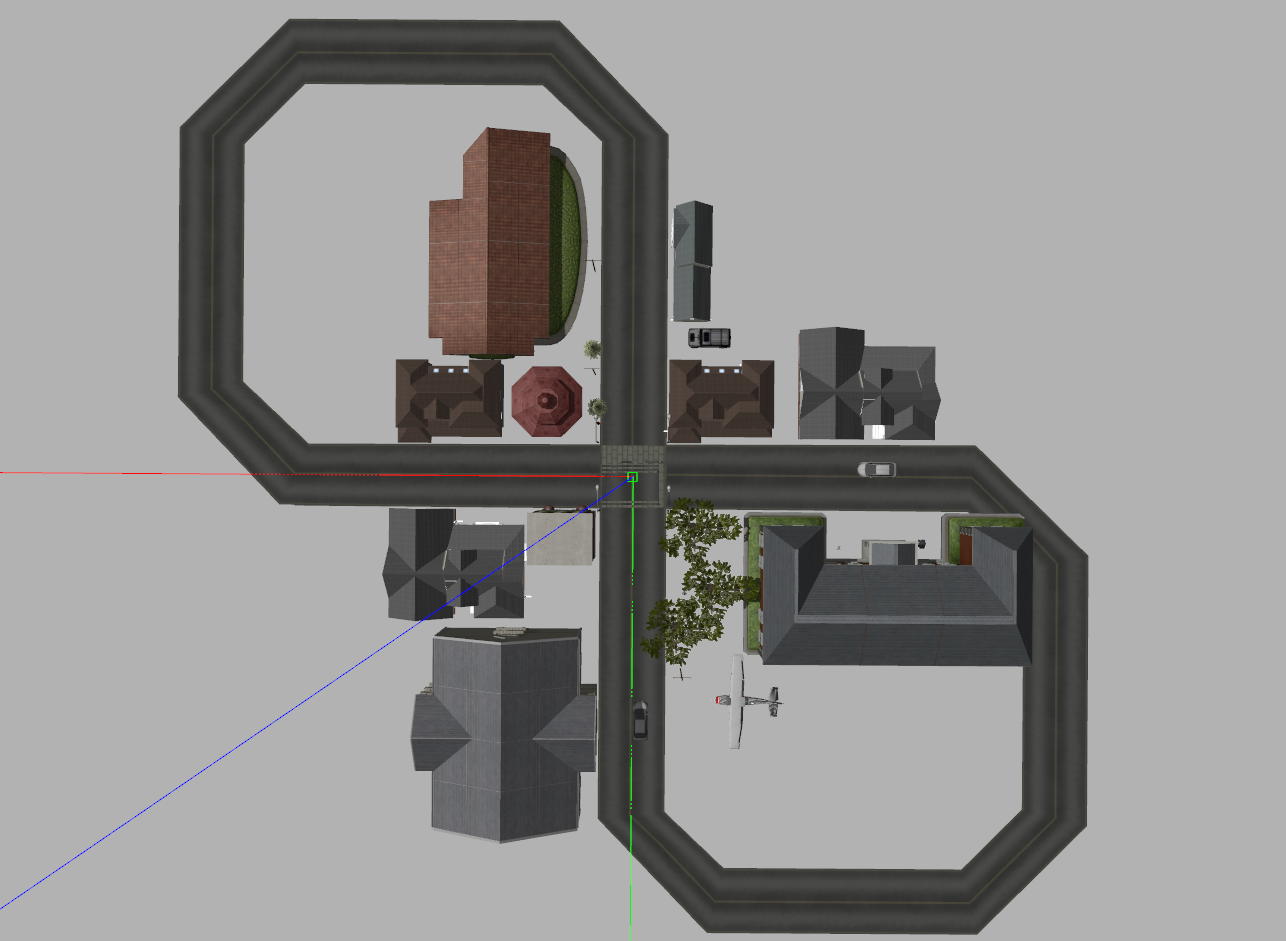
\includegraphics[width=0.7\paperwidth]{GazeboCrossroad.png}}
\end{center}
\caption{The simulated crossroad scenario in the Gazebo simulator.}
\label{fig:GazeboCrossroad} 
\end{figure}

The validity of the proposed model is done at a simulated environment in Gazebo\footnote{an open source software that features 3 dimensions robotics simulator.} as shown in Fig.~\ref{fig:GazeboCrossroad}. Vehicles in the virtual world are controlled through the ROS\footnote{short for "Robot Operating System", is a robotics middle-ware that provide users with integrated packages, services and tools} interface. The front, left and right views from the driver seat are directly projected onto the screens when driving in simulated world as in Fig.~\ref{fig:FrontCam}, Fig.~\ref{fig:LeftCam} and Fig.~\ref{fig:RightCam} respectively. Control commands from the volunteers are sent from the joysticks to ROS node to control the simulated vehicle in Gazebo. In every set of interaction experiments, a pair of volunteers (as shown in Fig.~\ref{fig:Driver1} and Fig.~\ref{fig:Driver2}) are asked to drive across the intersection without collision. The displacements to the node and the speed of vehicles for both driver are recorded with the time resolution of 0.01 sec. 

\begin{figure}[htbp!]
    \centering
    \subfloat[Left camera from driver seat in the simulated environment.]
    {
    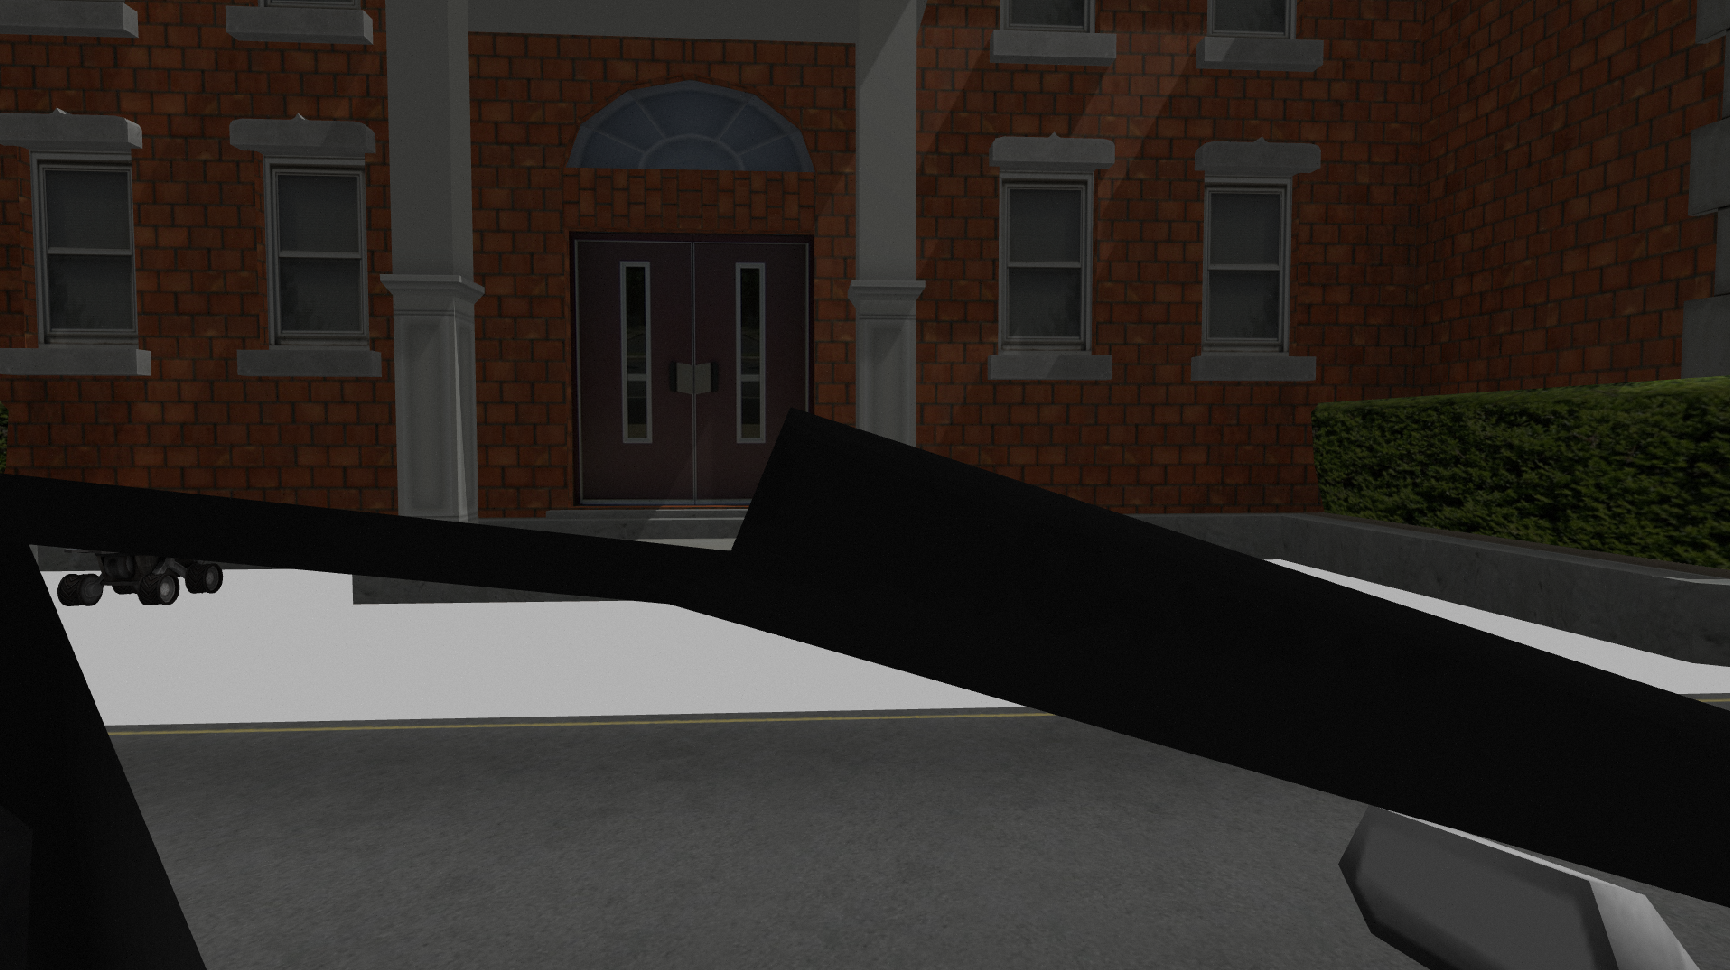
\includegraphics[width=0.47\textwidth]{PriusLcam.png}
    \label{fig:LeftCam}
    }\hfill
    \subfloat[Right camera from driver seat in the simulated environment.]
    {
    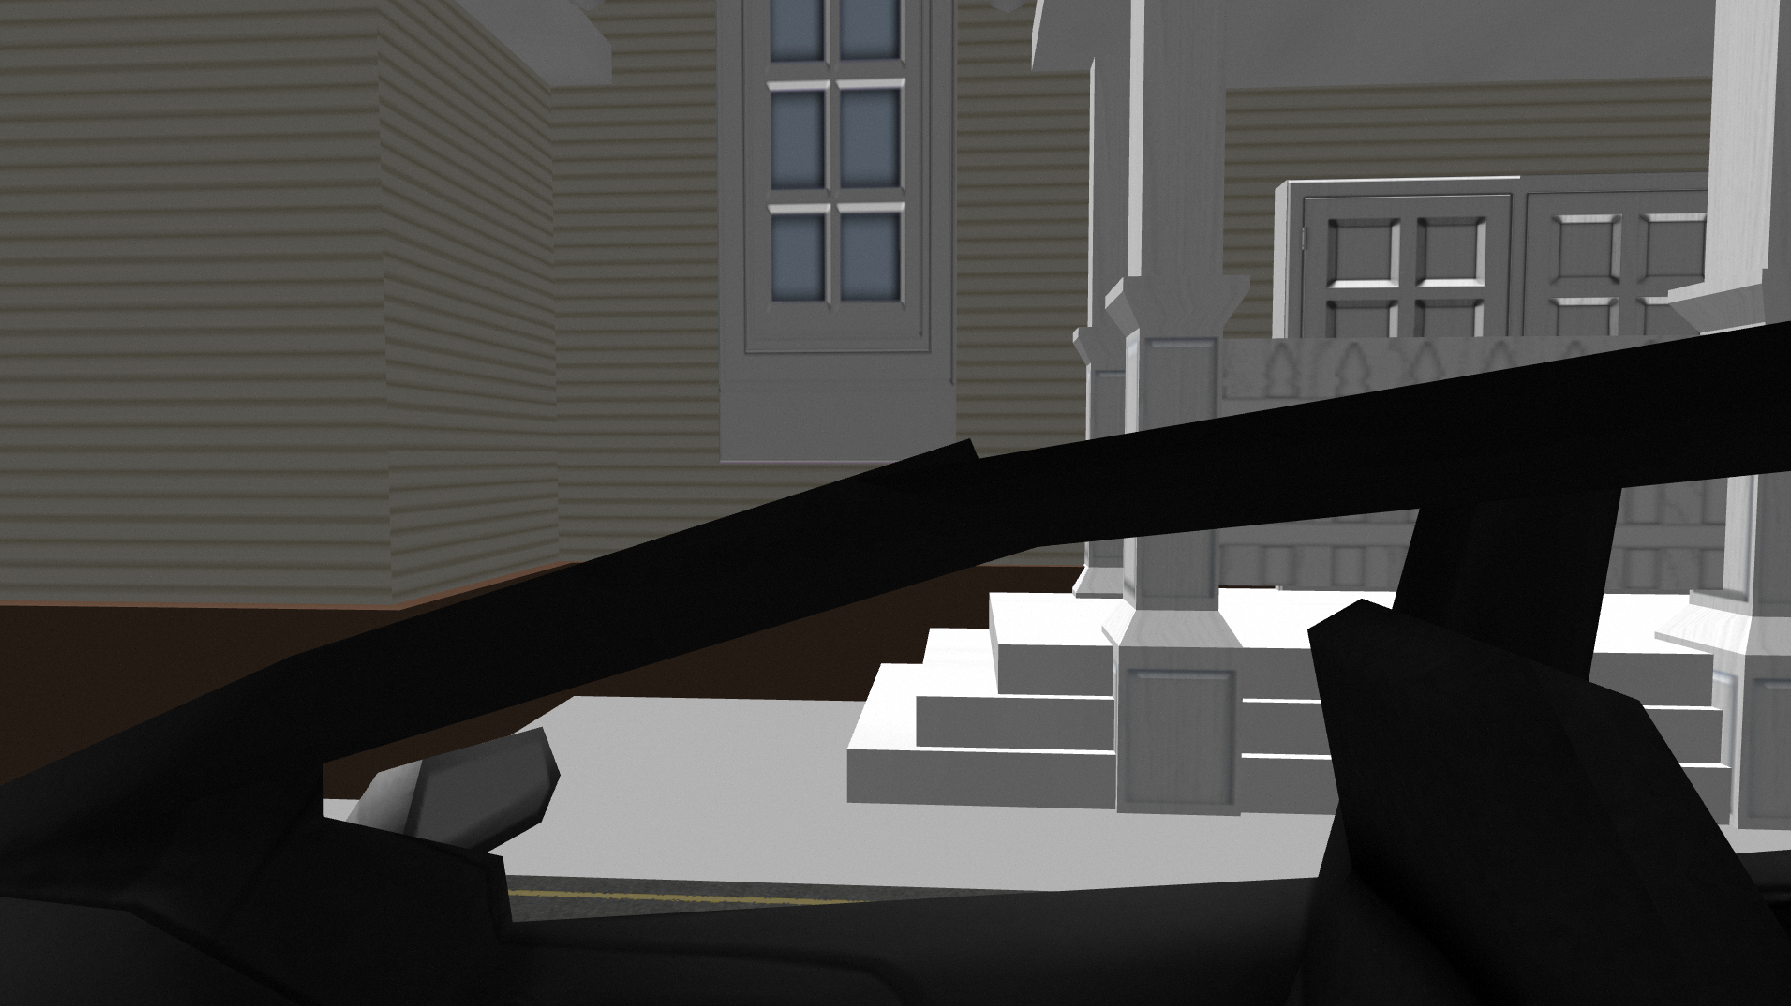
\includegraphics[width=0.47\textwidth]{PriusRcam.png}
    \label{fig:RightCam}
    }\hfill
    \subfloat[Front camera from driver seat in the simulated environment.]
    {
    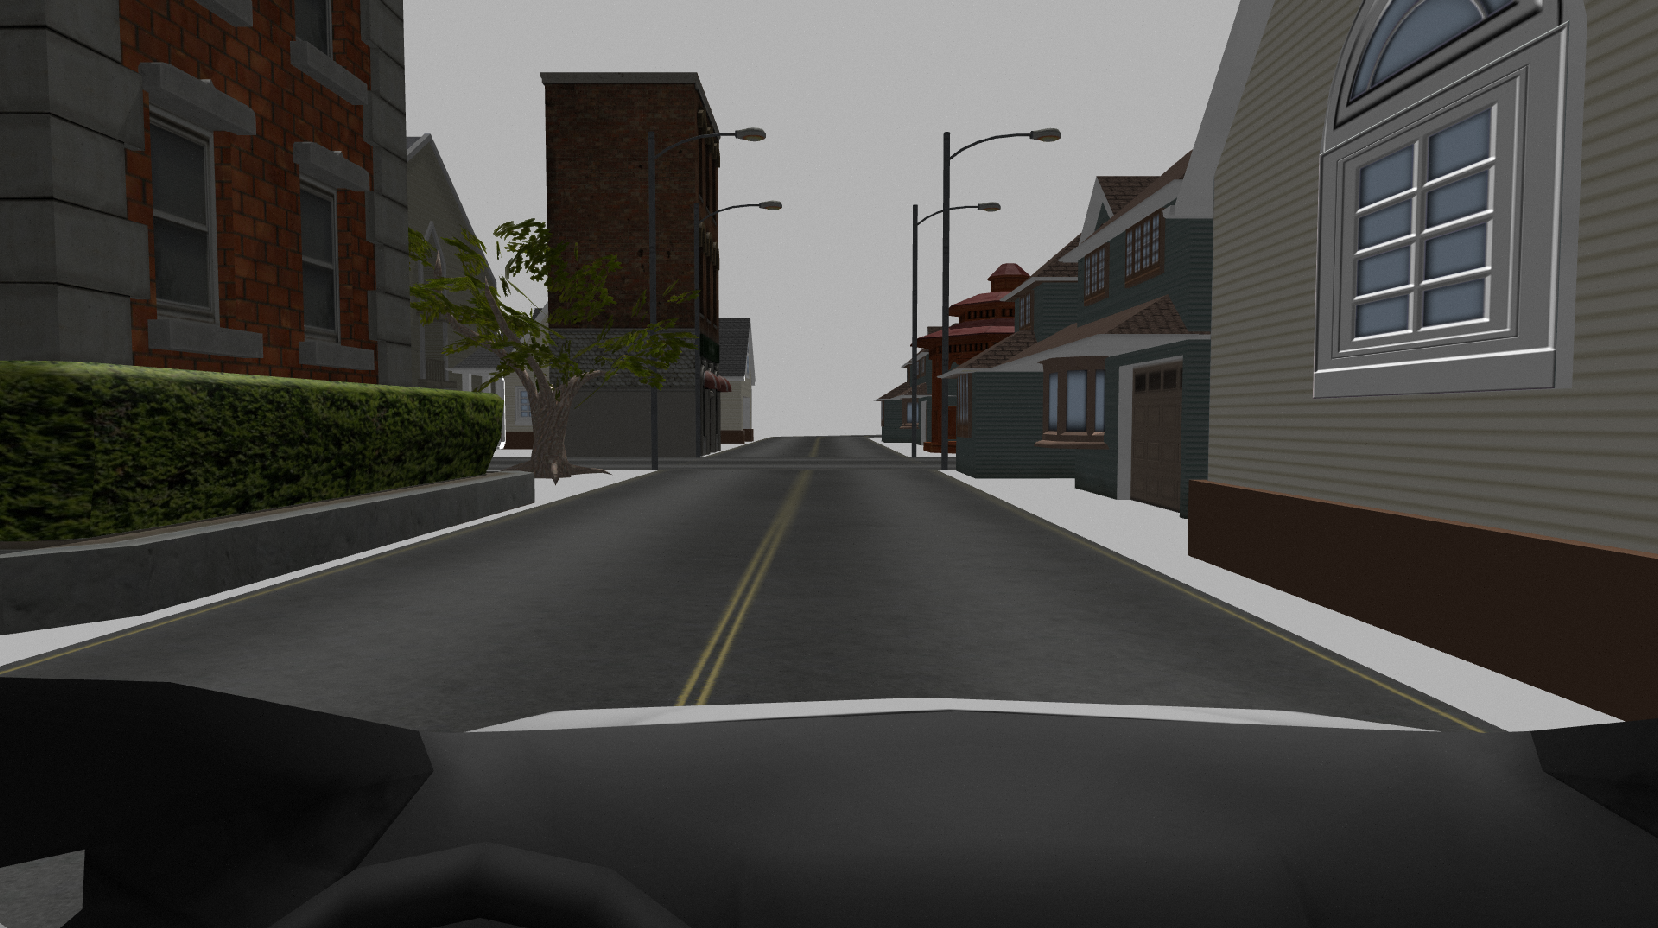
\includegraphics[width=0.47\textwidth]{PriusFcam.png}
    \label{fig:FrontCam}
    }\hfill
    \caption{Views from driver seat in the simulated environment.} \label{fig:AllCam}
\end{figure}

\begin{figure}[htbp!]
    \centering
    \subfloat[First driver in the simulated crossroad interaction experiment.]
    {
    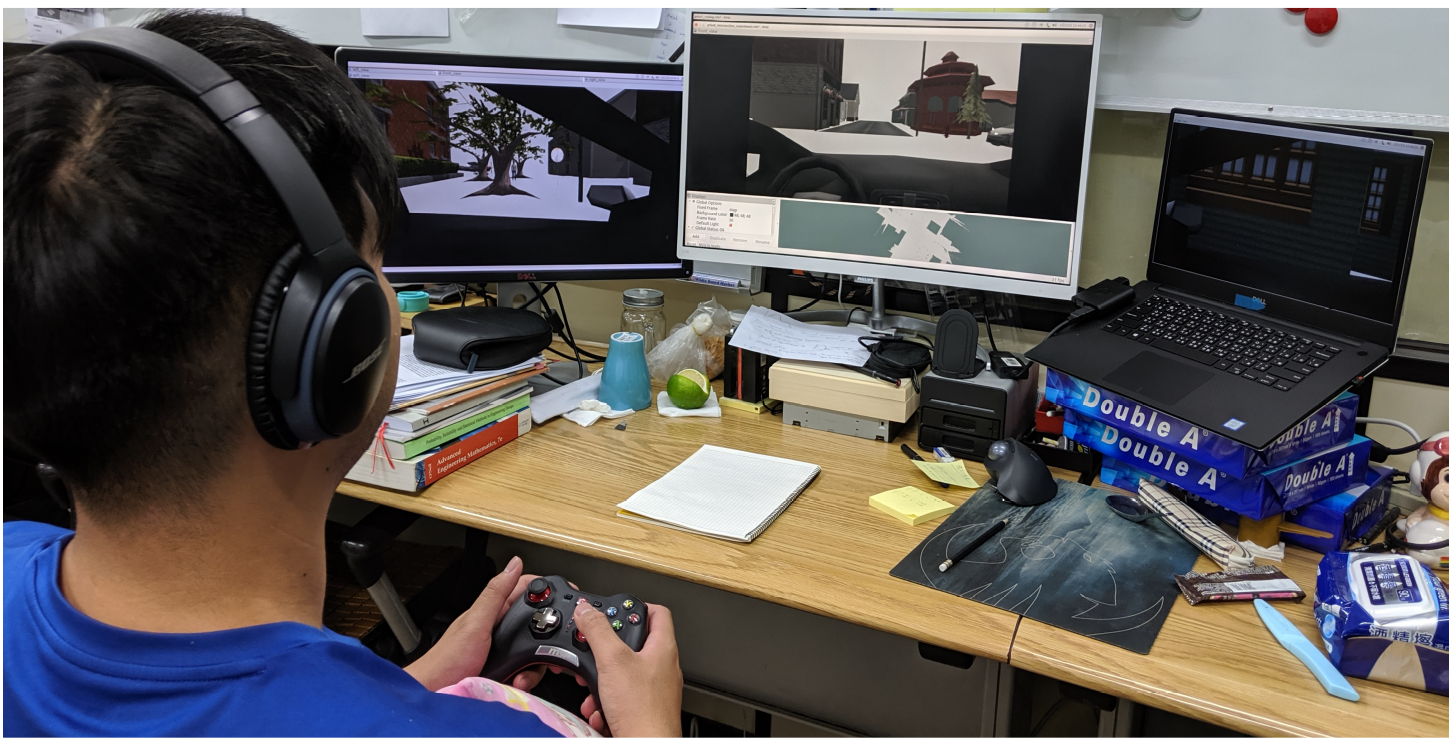
\includegraphics[width=0.47\textwidth]{Driver1.png}
    \label{fig:Driver1}
    }\hfill
    \subfloat[Second driver in the simulated crossroad interaction experiment.]
    {
    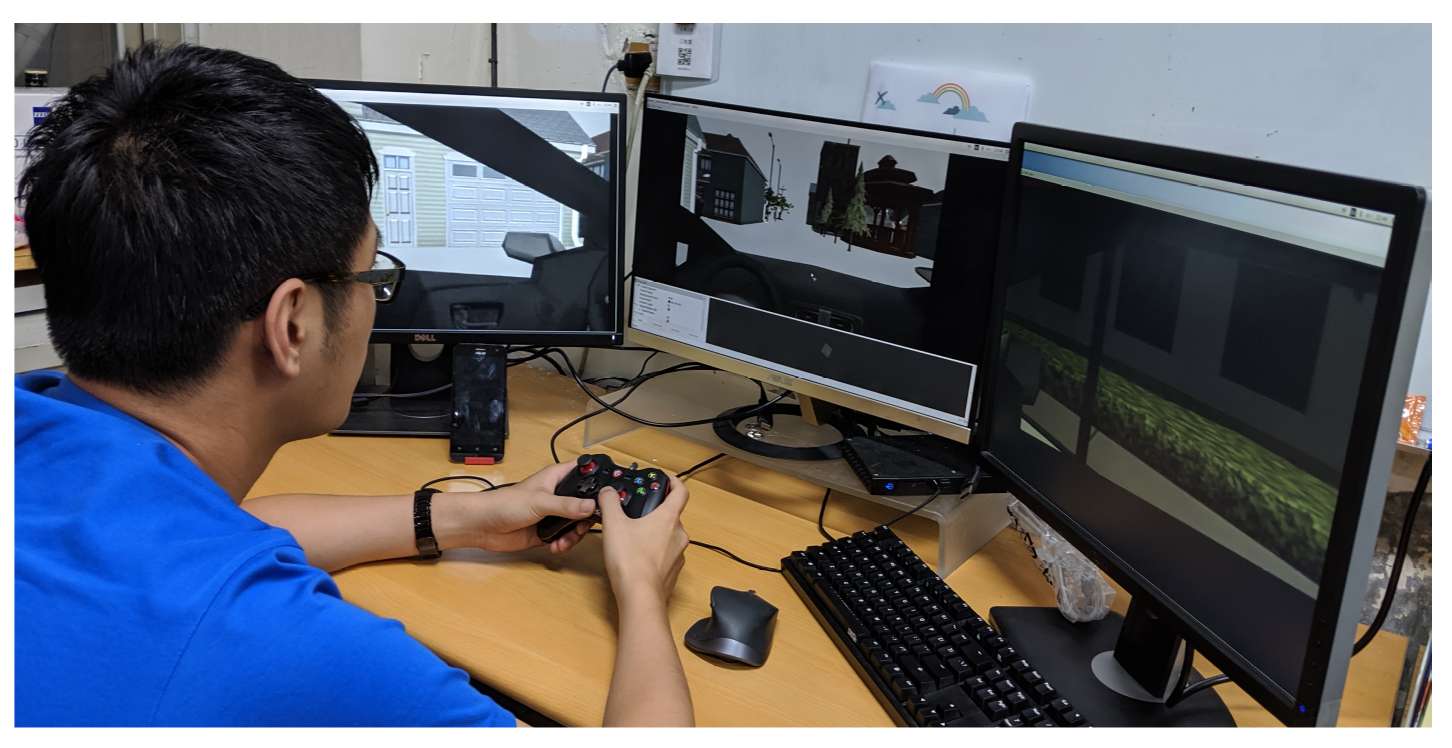
\includegraphics[width=0.47\textwidth]{Driver2.png}
    \label{fig:Driver2}
    }\hfill
    \caption{Volunteers in the simulated crossroad interaction experiment.} \label{fig:Drivers}
\end{figure}

We recorded 150 sets of data (labeled with number, e.g. \#001, \#002, ...) with the velocity $v_i(t)$, and the displacement to the node $d_{\mathrm{node},i}(t)$ of both vehicles. For all experiments, $t$ begins when either of the participants is 20 meters away from the node, which is the longest distance drivers can see each other, and ends when one of the vehicle reaches the node. The corresponding TTC of car\_0 and car\_1 are then calculated, as illustrated in Fig.~\ref{fig:figure_explaination_TTC} at $t_A$, $t_B$, $t_C$, $t_D$ and $t_E$. The probability of stopping for each car is plotted with the velocity and the displacement, as illustrated in Fig.~\ref{fig:figure_explaination_1}. 

%In the following paragraph, some cases will be explained in detail to demonstrate the performance of the proposed model. Finally, the classification accuracy rate will be evaluated using all data sets for validation.  

\begin{figure}[htbp!]
    \centering
    \subfloat[Illustration of calculated TTC of each vehicle.]
    {
    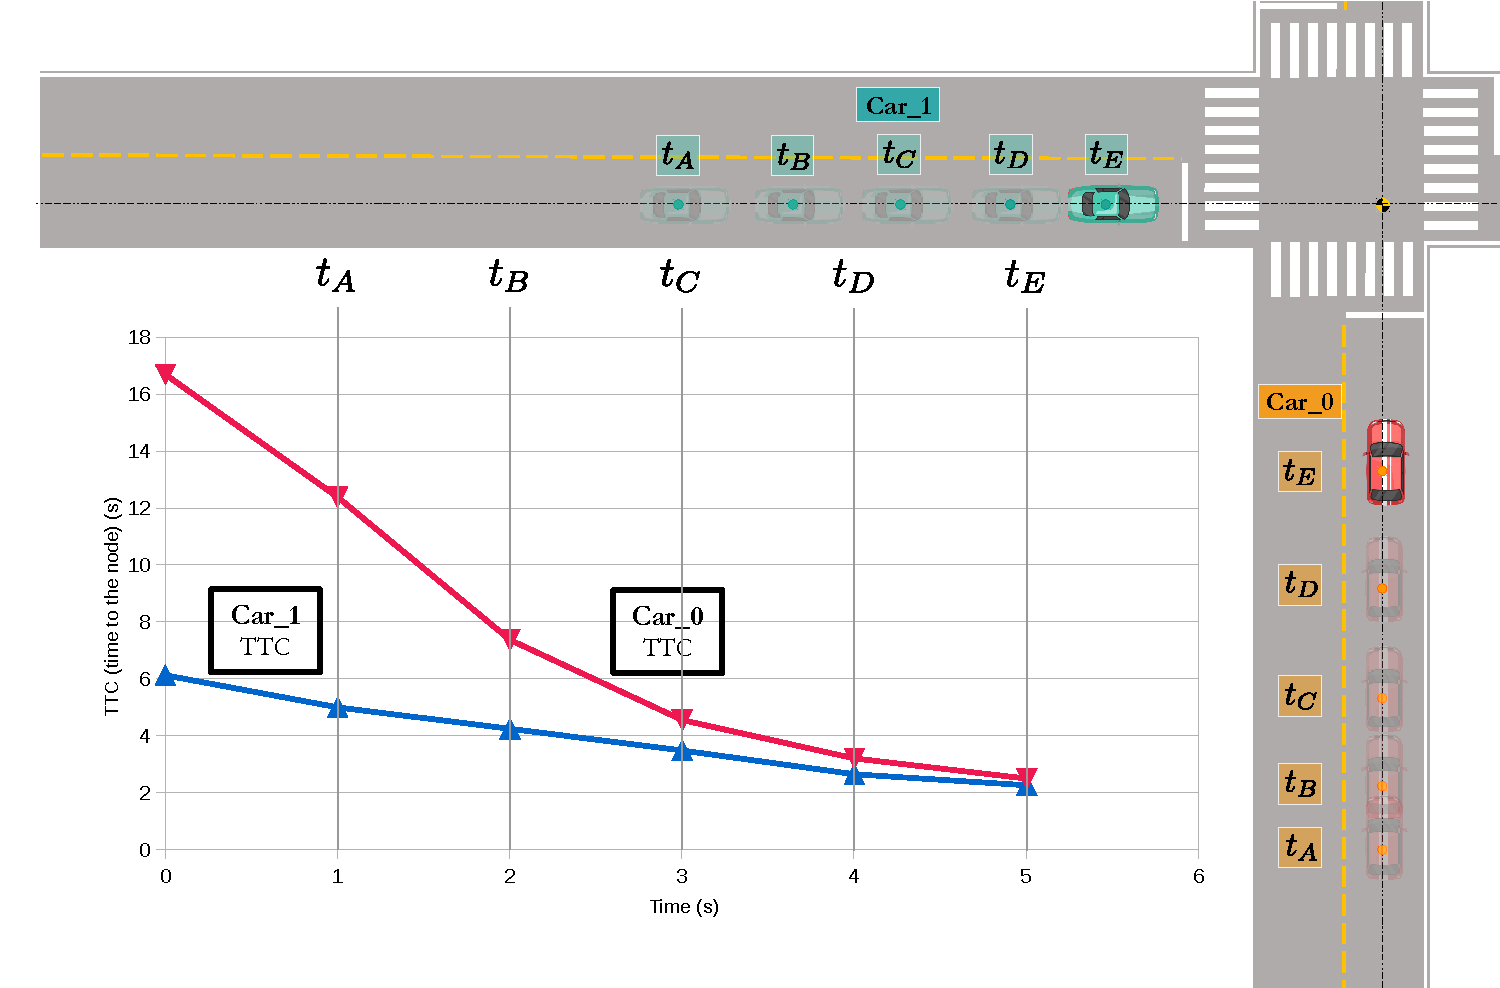
\includegraphics[width=0.47\textwidth]{figure_explaination_TTC.pdf}
    \label{fig:figure_explaination_TTC}
    }\hfill
    \subfloat[Illustration of probability of stopping together with velocity and displacement.]
    {
    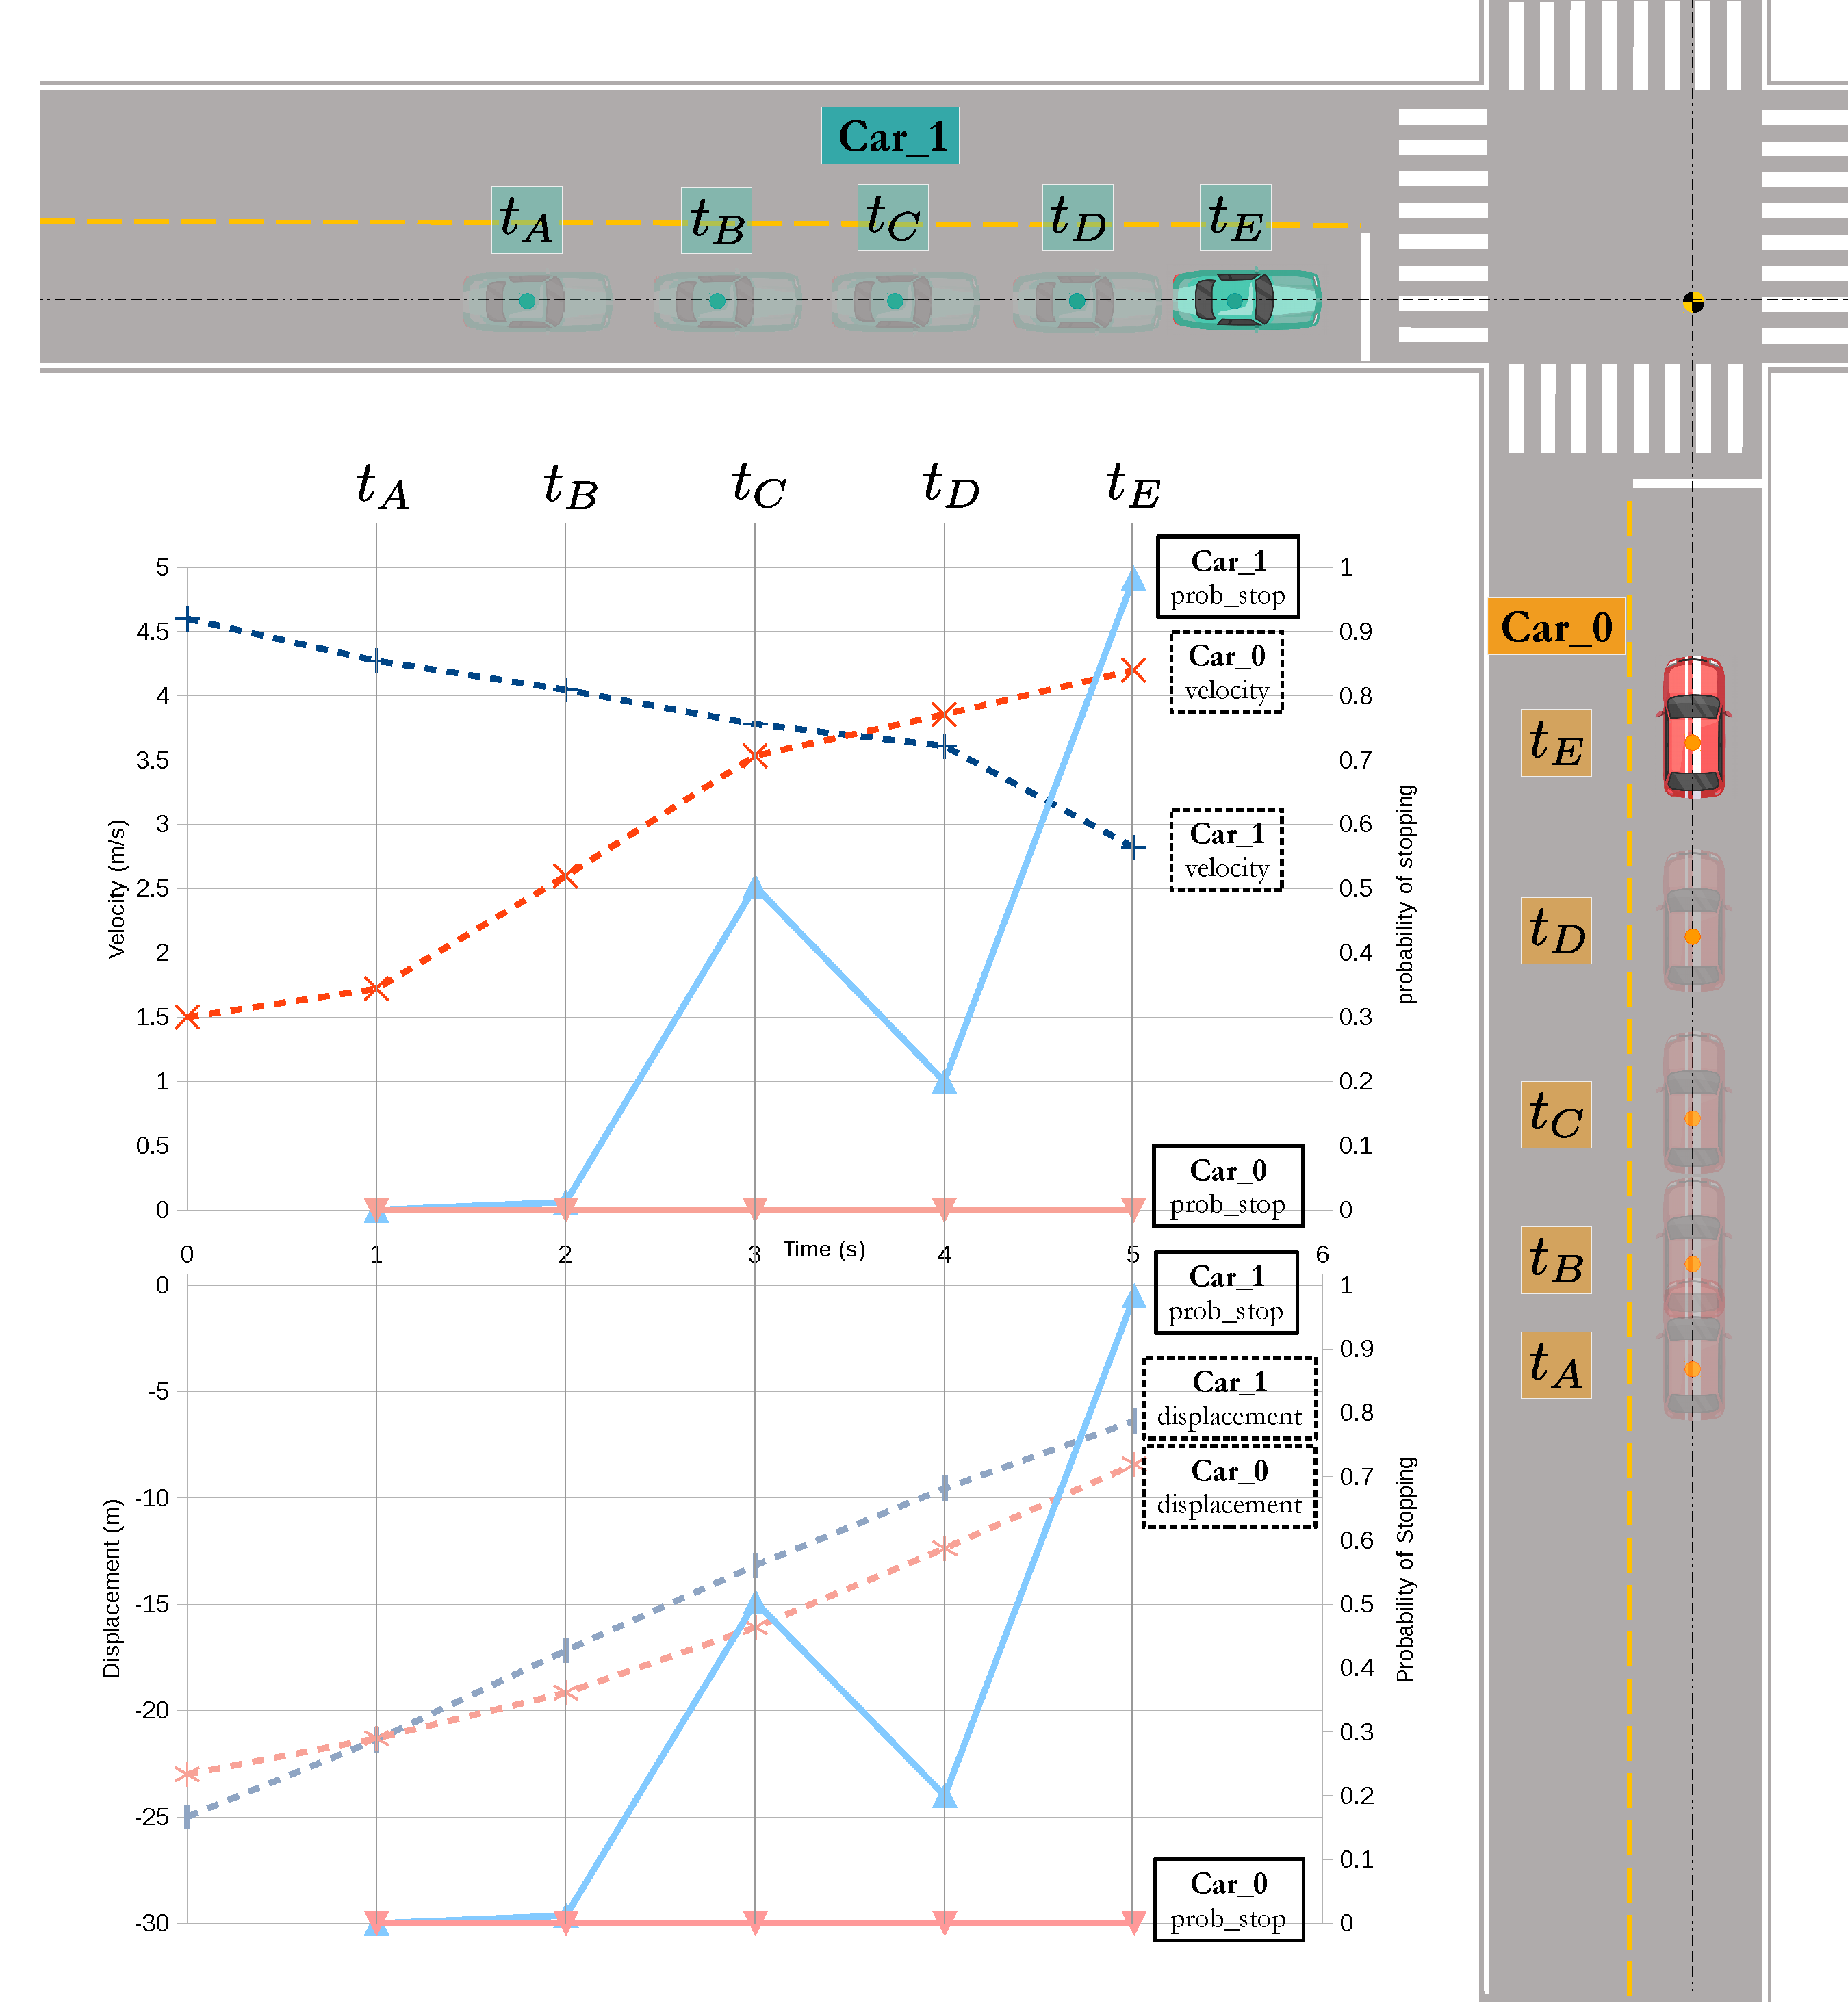
\includegraphics[width=0.47\textwidth]{figure_explaination_1.pdf}
    \label{fig:figure_explaination_1}
    }\hfill
    
    \caption{Illustration of TTC and probability of stopping along with concerning variables.} \label{fig:illustration}
\end{figure}

\newpage

Let us look at the experiment \#063 in Fig.~\ref{fig:trial063}. car\_0 was 21 meters to the node compared with 25 meter for car\_1. At $t=1.3$ seconds, the POY of car\_0 increases therefore the driver slows down to yield to car\_1 who at the moment had no intention to yield. The entire process can be reviewed clearly using POY. In this experiment without providing the POY of car\_0 to car\_1, car\_1 chose to yield too to avoid potential collision. If the intention for car\_0 is given as a reference, unnecessary braking of car\_1 could have been avoided.


\begin{figure}[htbp!]
\begin{center}
\makebox[0pt]{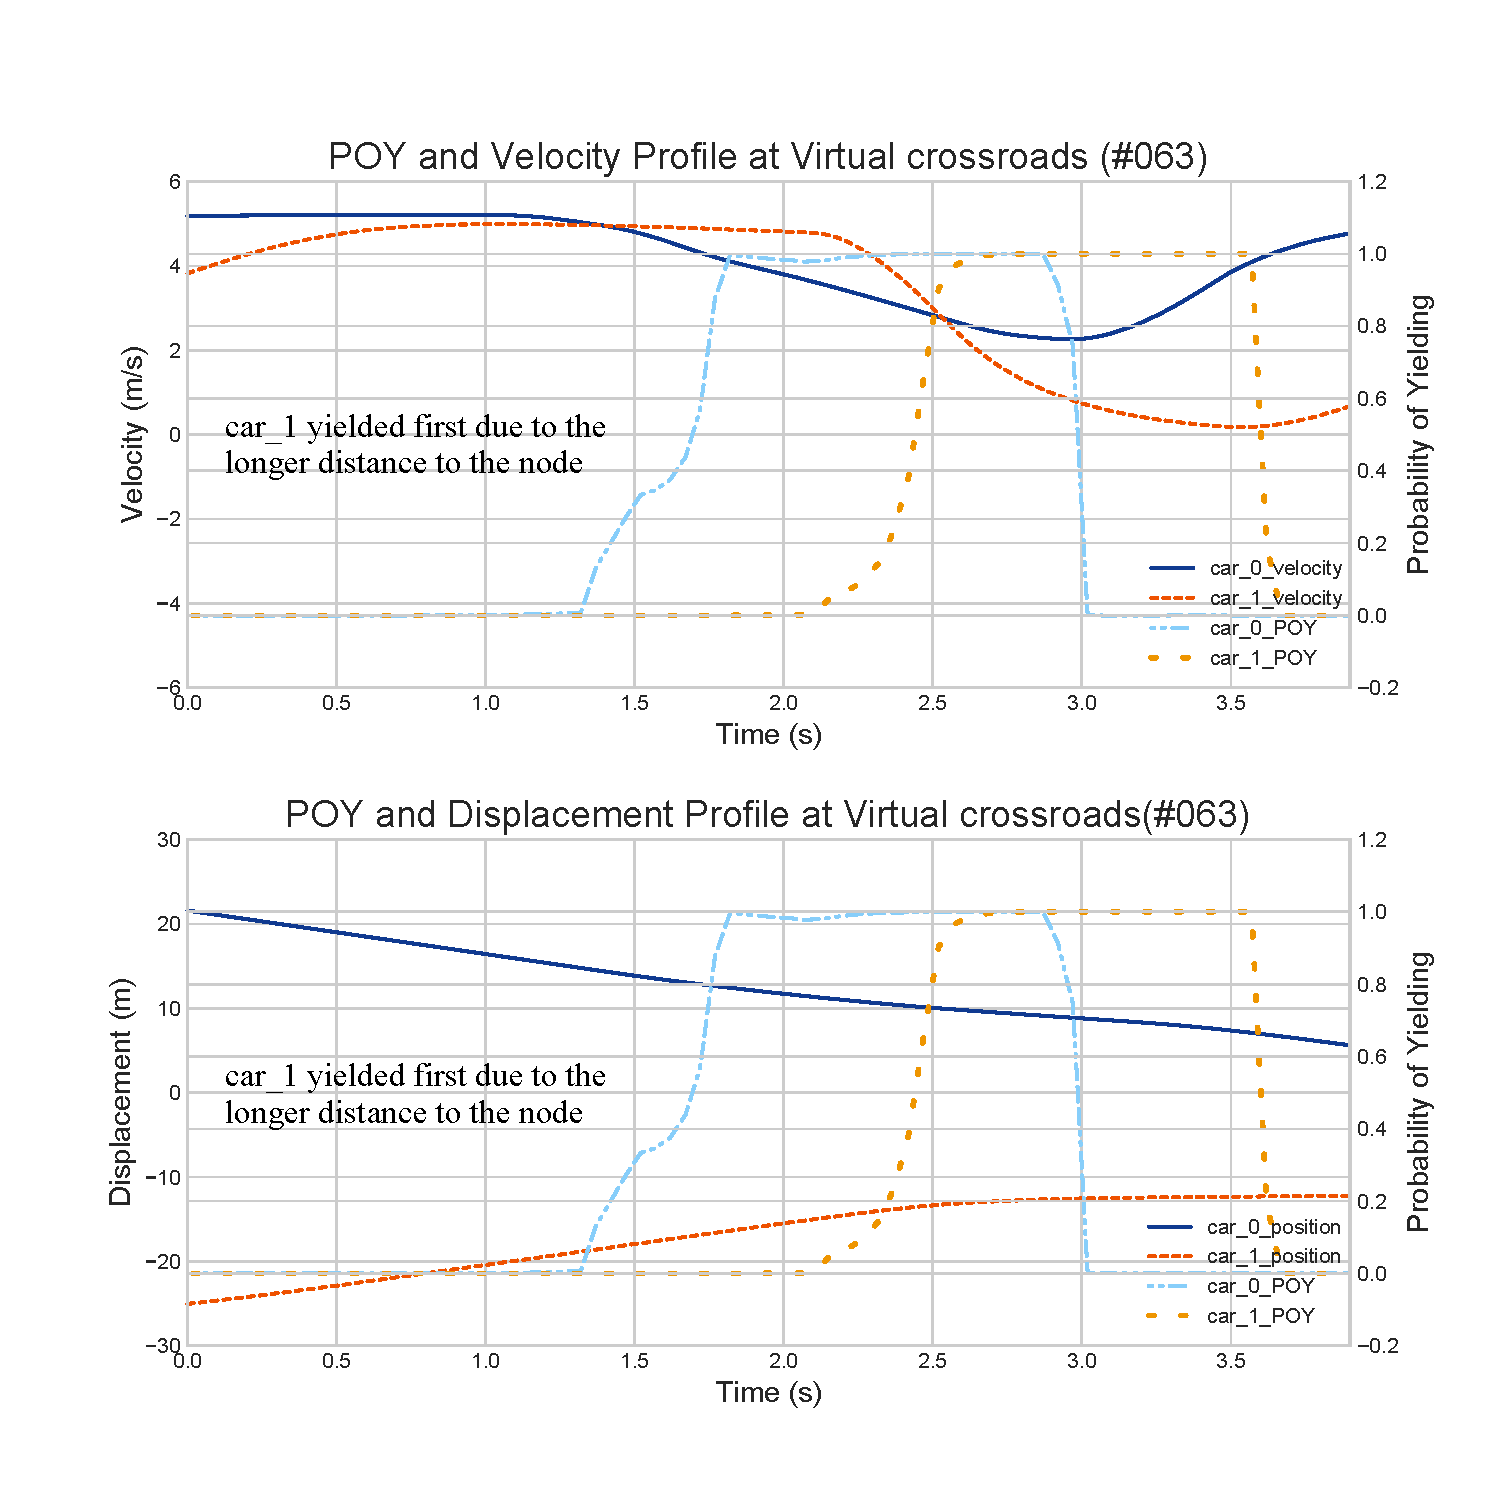
\includegraphics[width=0.85\paperwidth]{trial_063_bothyield.pdf}}
\end{center}
\caption{Trial \#063 where car\_0 yielded first but then passed due to the deceleration of car\_1 .}
\label{fig:trial063} 
\end{figure}

Now let us look at another case \#077, as shown in Fig.~\ref{fig:trial077}, where both drivers were indecisive without being dominate in position or other states. At the beginning of the interaction, POYs of both vehicles rose due to their deceleration. From $t=1.5$ to $3.2$ secs, the POYs were kept at high level for car\_0, while car\_1 had no intention to yield. But right after car\_1 accelerated, so did car\_0 with very small time difference (0.5 sec). And after about a second, they both decelerated together again, but this time car\_1 was determined to yield and car\_0 finally passed. During this time, human drivers had no information about what actions the other one intended to take, so they waited until one of them did something. Yet, if one could utilize the proposed model which could estimate the TFA distribution of the driver and generate a probability from his or her current states, this stand-off-like situation could have been avoided. In the most extreme case, it will take both drivers quite a long time before either one decides to pass or yield. In trial \#077, however, it did not take them too long before car\_0 finally decide to pass.  

\begin{figure}[htbp!]
\begin{center}
\makebox[0pt]{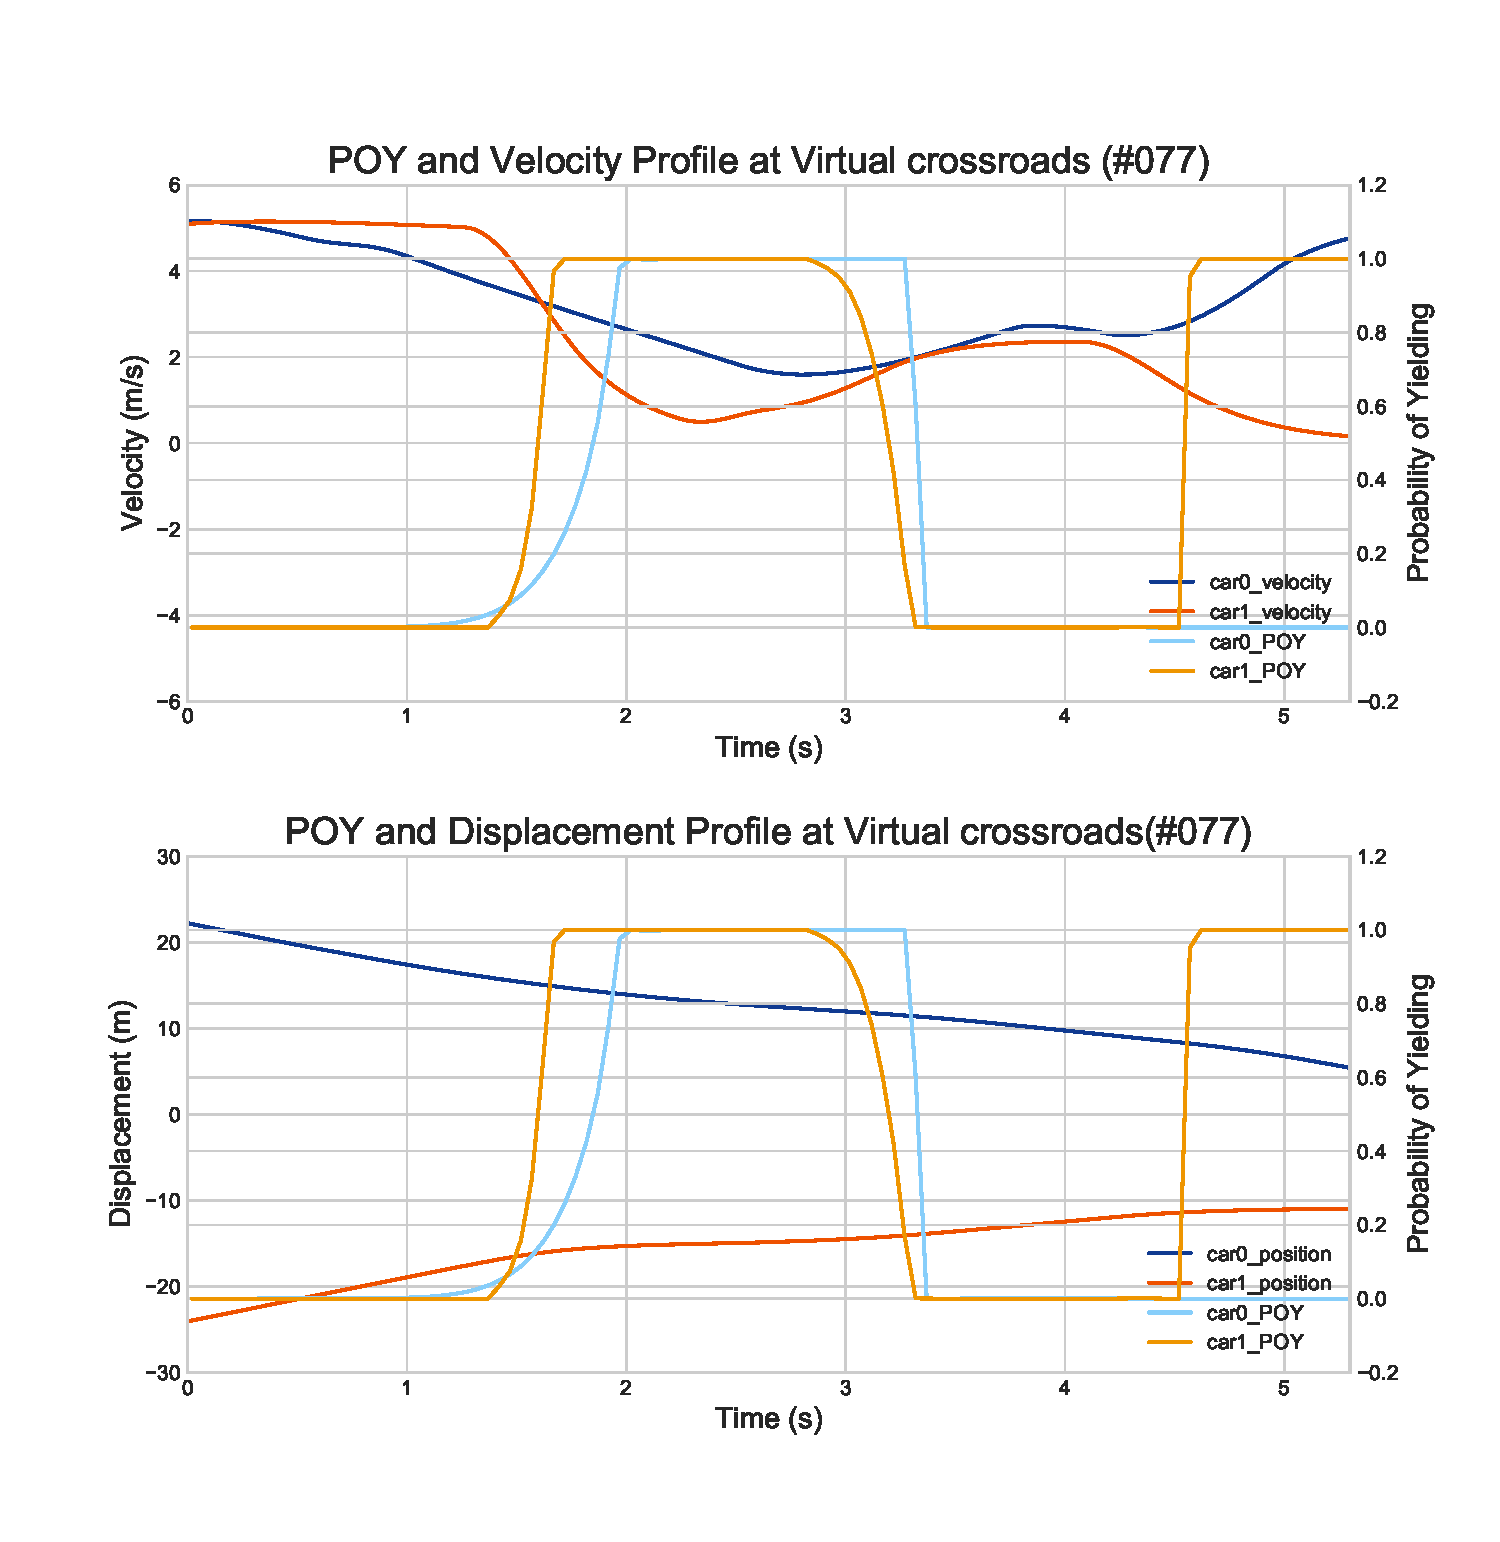
\includegraphics[width=0.85\paperwidth]{trial_077_indecisive.pdf}}
\end{center}
\caption{Trial \#077 where car\_0 and car\_1 were confused about what action the other one might take.}
\label{fig:trial077} 
\end{figure}

\newpage

In addition to the simulated environment, data at a real crossroad are also conducted to verify whether the proposed POY model can describe the driver behaviors in the real world. To collect the related data, the drone for aerial filming is used at the crossroad in urban environment (\textit{Bo’ai Rd.93-85, Yuanlin City, Changhua County 510, Taiwan (23.958606, 120.573283)}).

\begin{figure}[htbp!]
\begin{center}
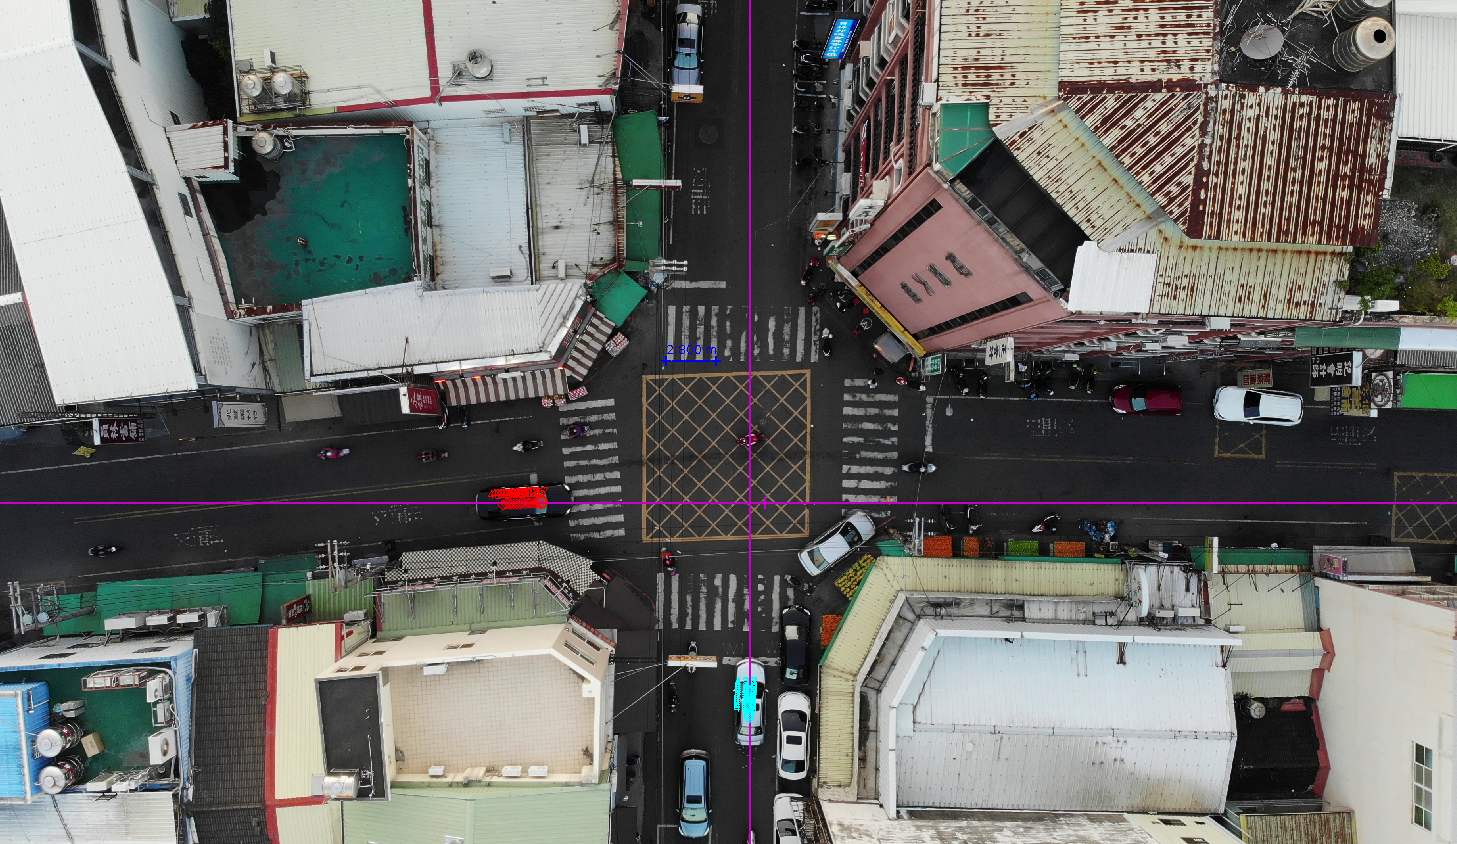
\includegraphics[scale=0.26]{aerial_filming_demo.png}
\end{center}
\caption{Using video analysis tool to track vehicles driven by humans.}
\label{aerial_filming} 
\end{figure}


\begin{figure}[htbp!]
\begin{center}
\makebox[0pt]{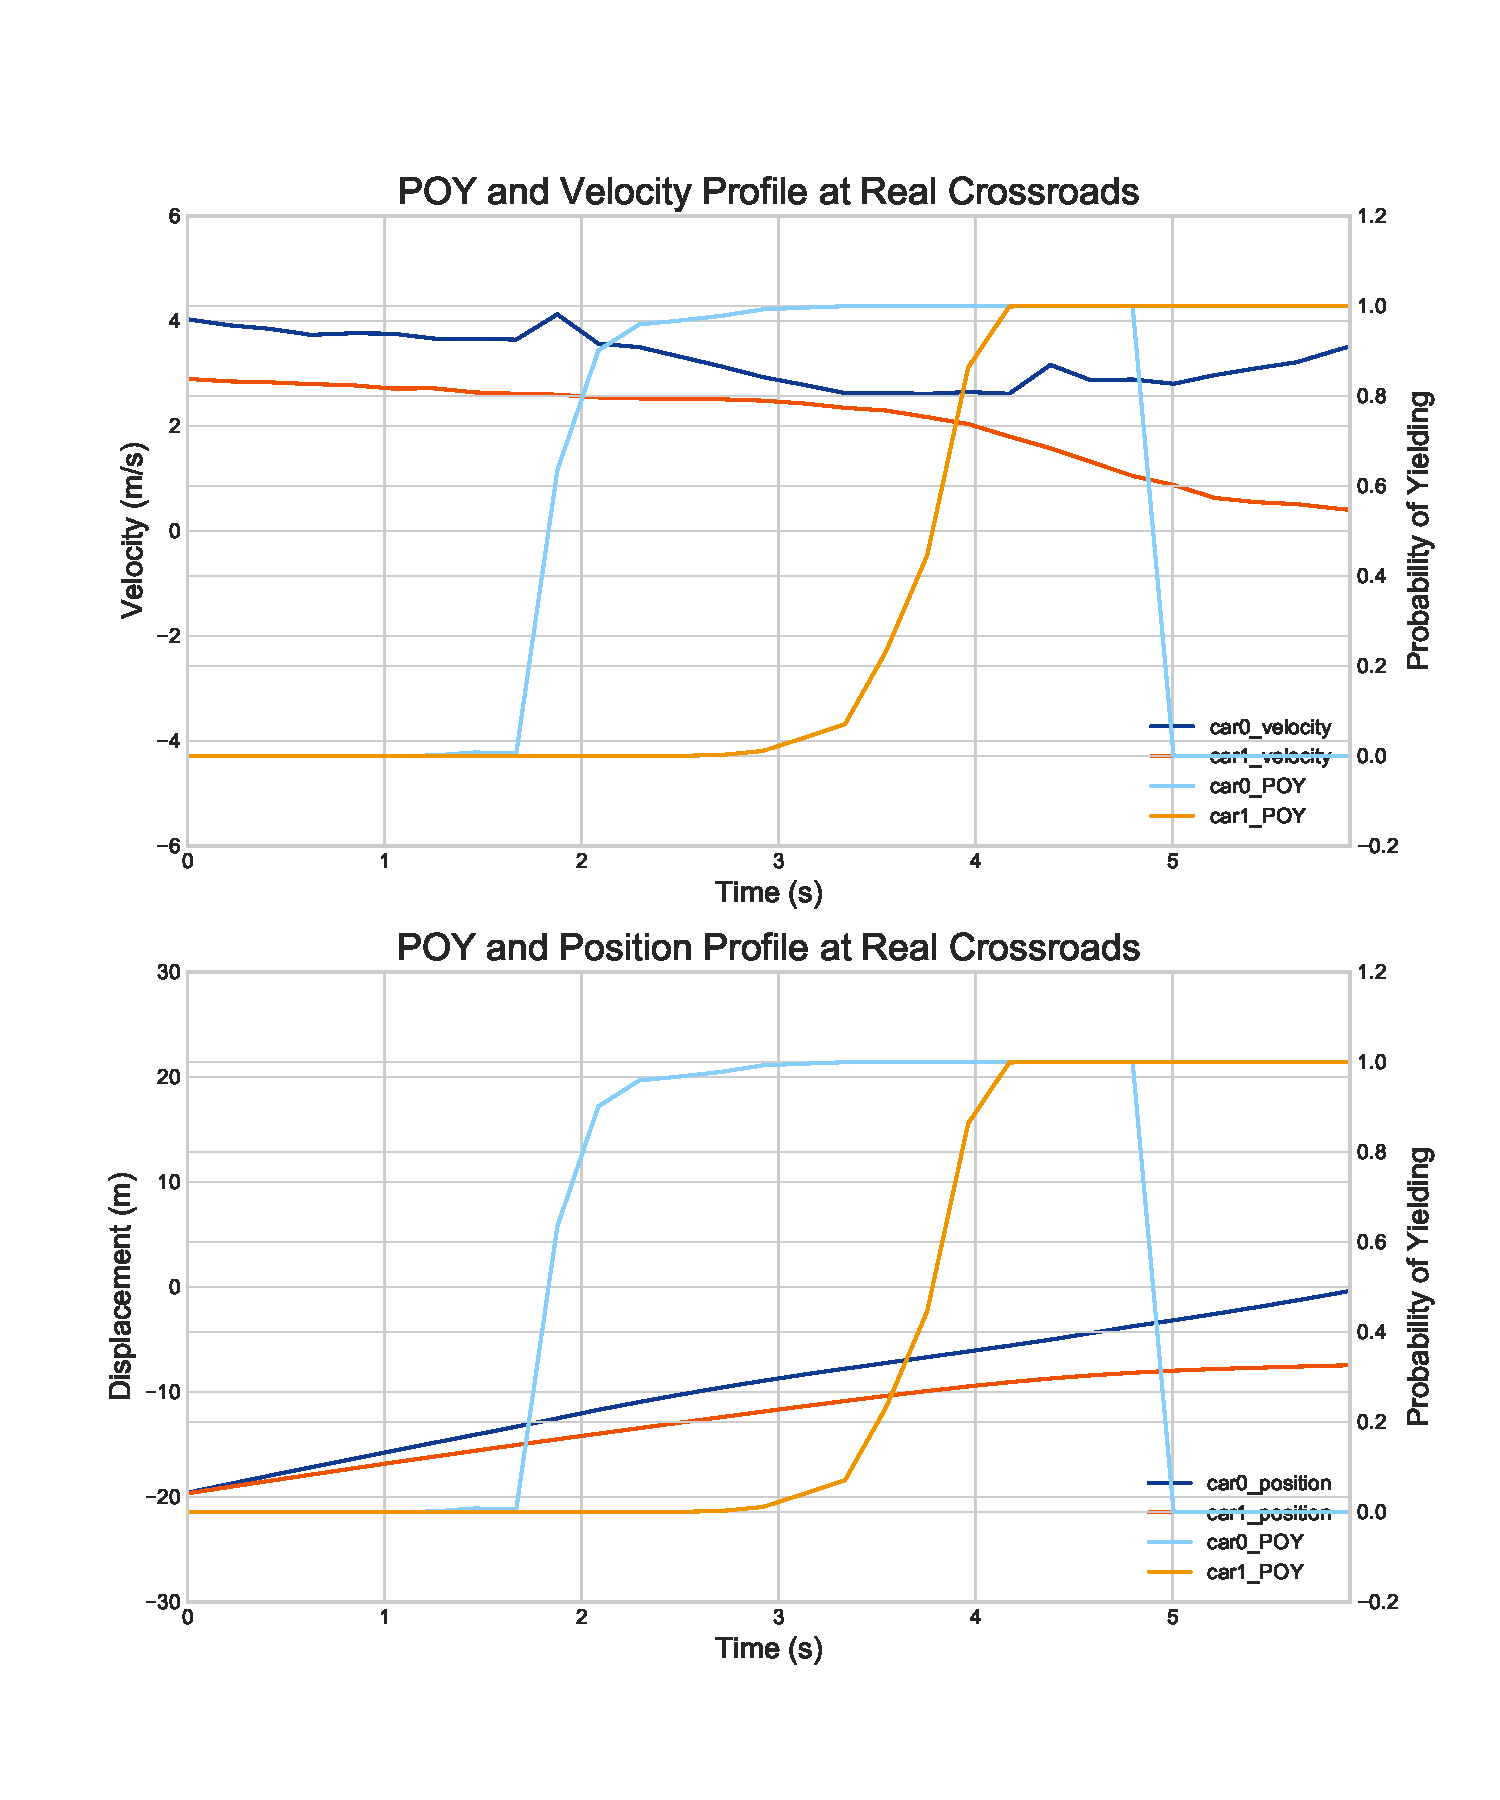
\includegraphics[width=0.85\paperwidth]{realworld_1.pdf}}
\end{center}
\caption{The corresponding POY curve at a crossroad in real world (Case I). car\_0 had the dominance position and passed at the end.}
\label{fig:POY_caseI} 
\end{figure}


\begin{figure}[htbp!]
\begin{center}
\makebox[0pt]{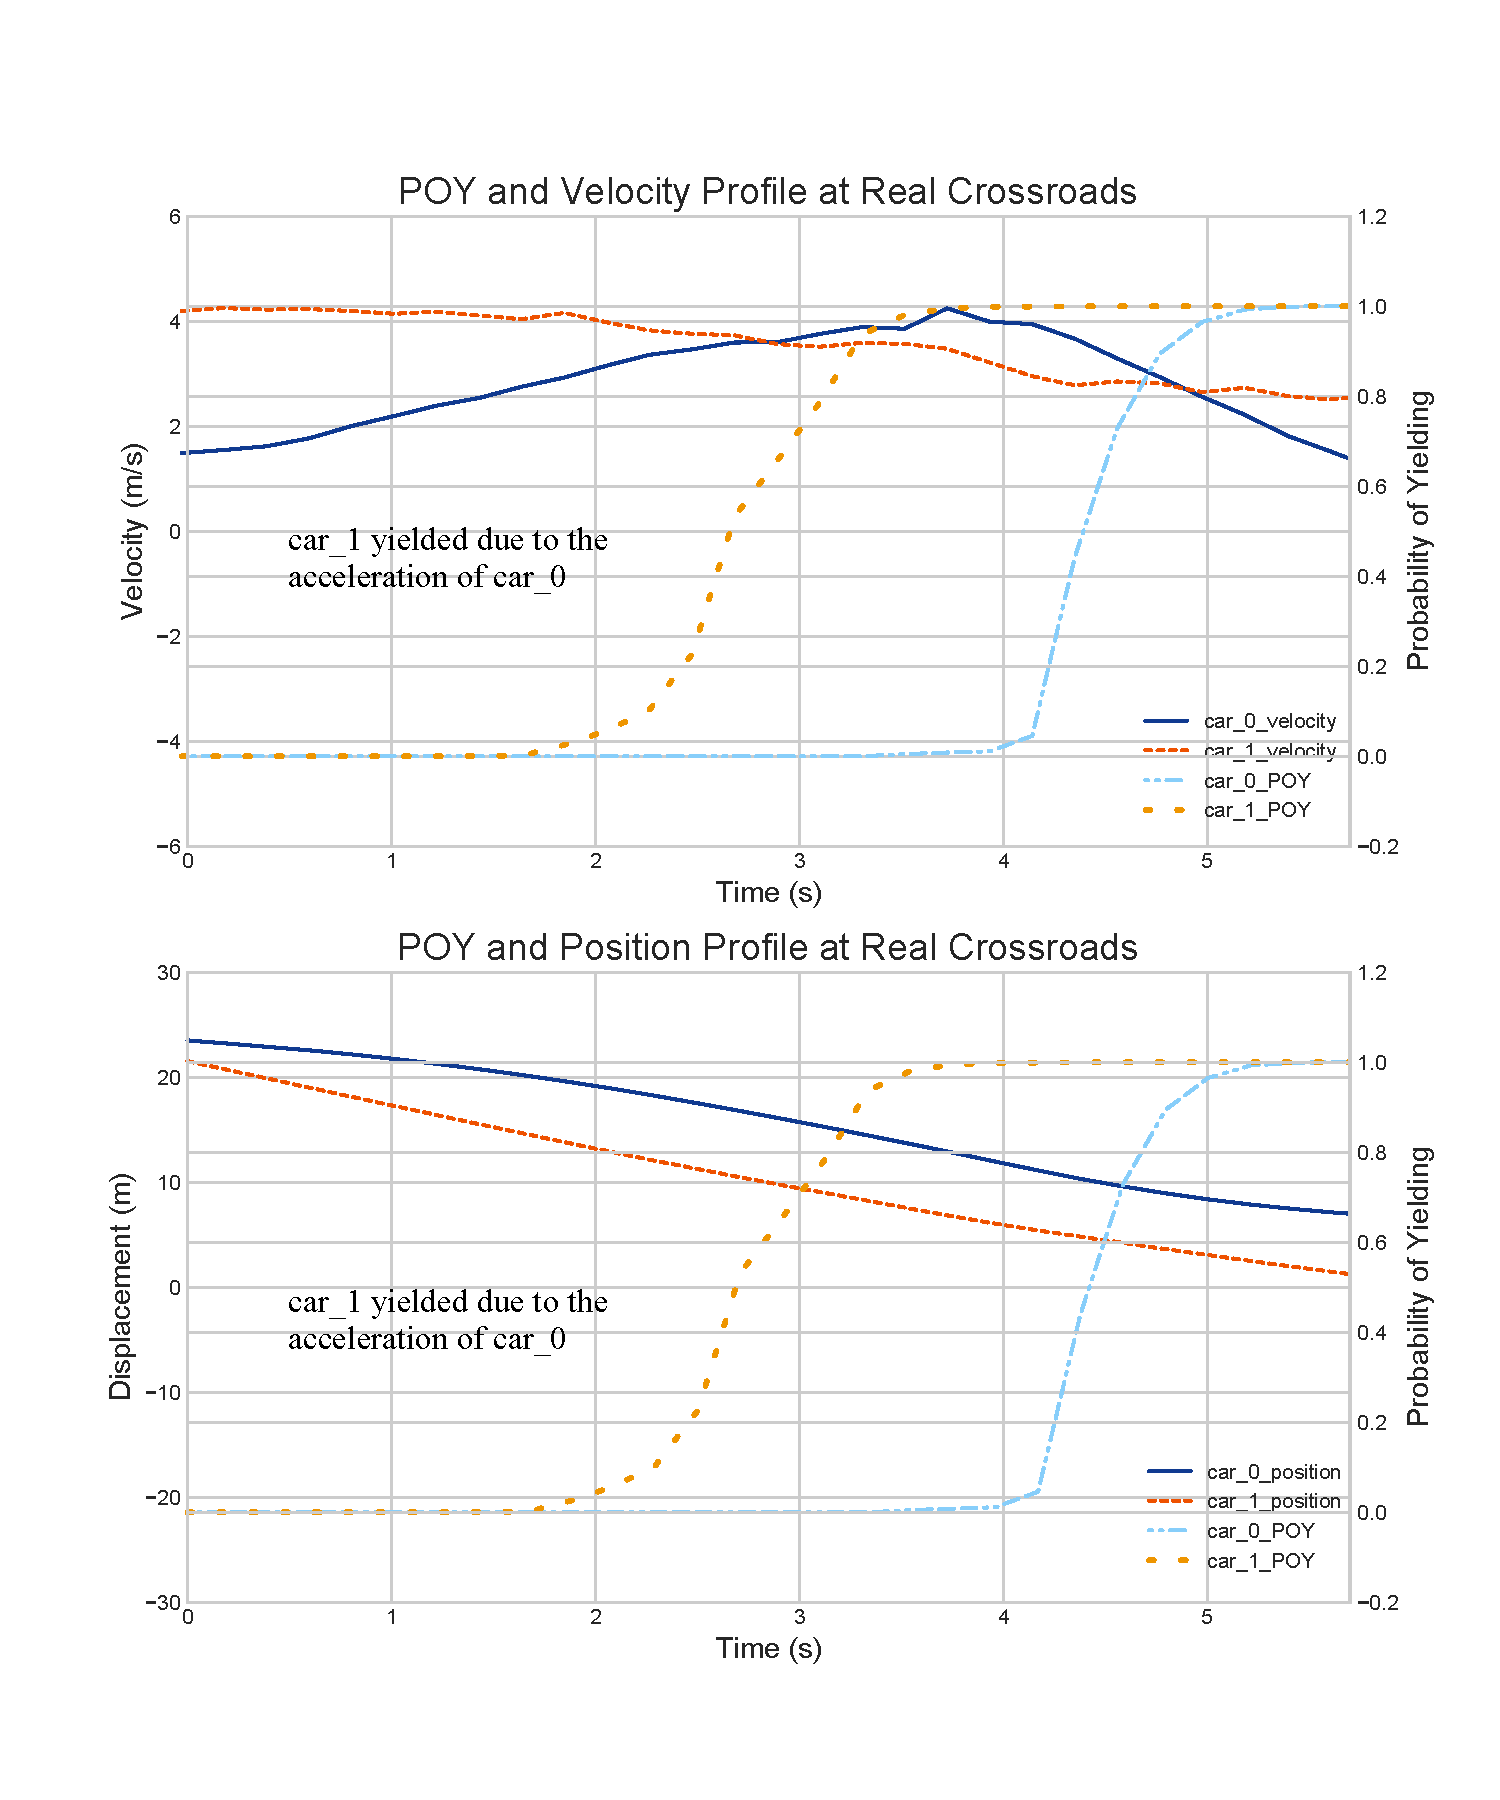
\includegraphics[width=0.85\paperwidth]{realworld_2.pdf}}
\end{center}
\caption{The corresponding POY curve at a crossroad in real world (Case II). car\_1 had the dominance position but yield at the end.}
\label{fig:POY_caseII} 
\end{figure}


Two of the interaction are shown in Fig.~\ref{fig:POY_caseI} and Fig.~\ref{fig:POY_caseII} where the POY curves are similar to those example trials in the virtual crossroads and are also comparable to human drivers' judgements. After examining the performance of the proposed model by comparing the POY curves to the predictions of human drivers, the accuracy of the proposed model will be examined.

\begin{equation}
    R_{\mathrm{CA}} = \frac{\text{number of correctly classified situations}}{\text{number of all situations}}
\label{eq:CARate}
\end{equation}

The $R_{\mathrm{CA}}$ is used to evaluate the calssification accuracy of the proposed model. Due to the fact that the time spans for all interaction trials are different, the time line is be reversed and denoted as $T_{\mathrm{minus}}$, i.e., $T_{\mathrm{minus}}=0$ denotes the time at the end of the process and $T_{\mathrm{minus}}=1$ denotes the time 1 sec earlier than that, and so on. Note that the end of the process is defined as the moment which the node is reached by one of the participants. The calculation of $R_{CA}$ is rather straight forward as shown in Eqn.(\ref{eq:CARate}). In the total of 168 cases of driver behaviors at the crossroad, the denominator of the $R_{\mathrm{CA}}$ at each $T_{\mathrm{minus}}$ is then 168. The $R_{\mathrm{CA}}$ results of the proposed model are shown in Fig.~\ref{fig:CARPOY}.

\begin{figure}[htbp!]
\begin{center}
\makebox[0pt]{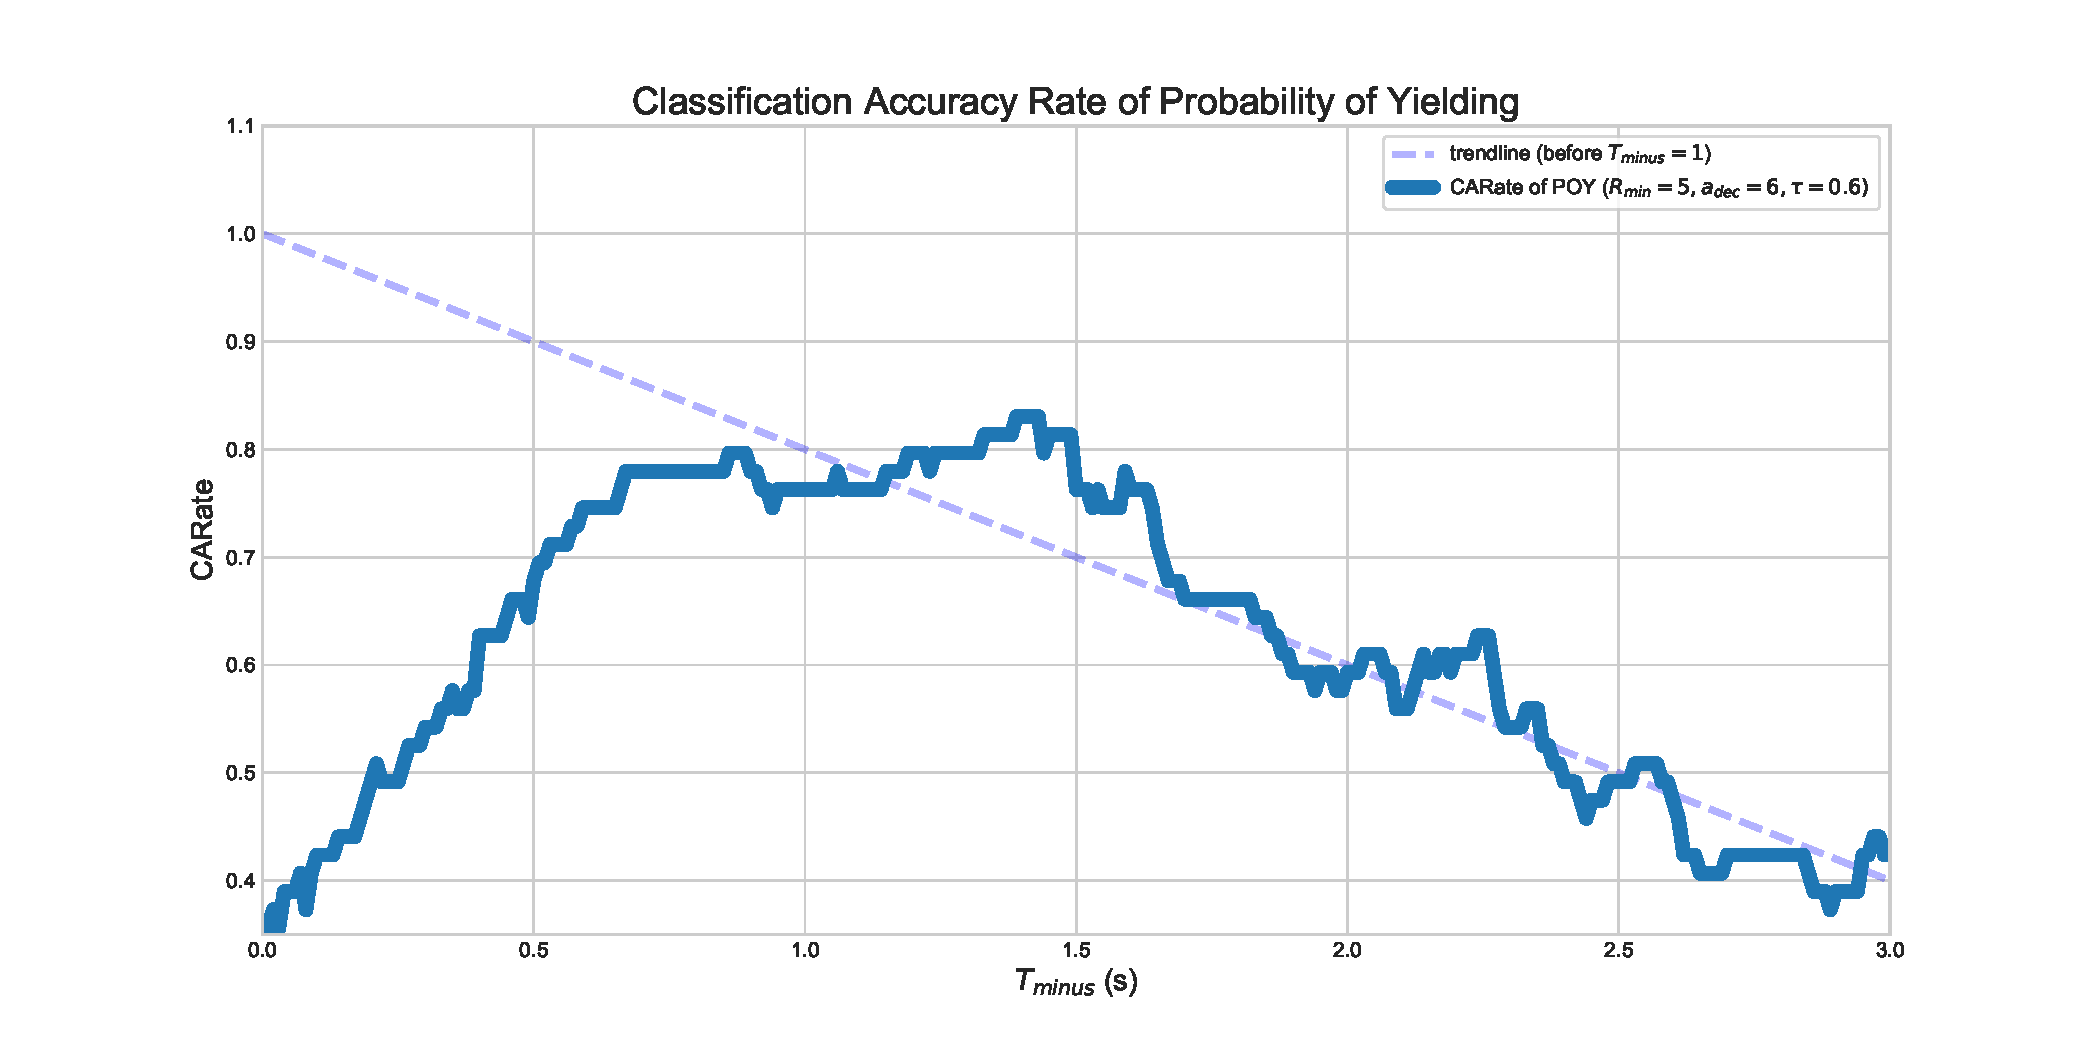
\includegraphics[width=0.85\paperwidth]{CARPOY.pdf}}
\end{center}
\caption{$R_{\mathrm{CA}}$ of the POY using all data sets.}
\label{fig:CARPOY} 
\end{figure}

Results using the average parameters listed in Table.~\ref{table:parameters} are plotted in solid blue line while the trend line is plotted in dashed blue line. The reason for the drop from 0.0 to 1.5 $T_{\mathrm{minus}}$ is that, people tend to behave more aggressive in our simulated environments. During the experiment, participants who yielded for the other driver accelerated before the end of the process which is the moment when the node is reached. The example is shown in Fig.~\ref{fig:trial039}.

\begin{figure}[htbp!]
\begin{center}
\makebox[0pt]{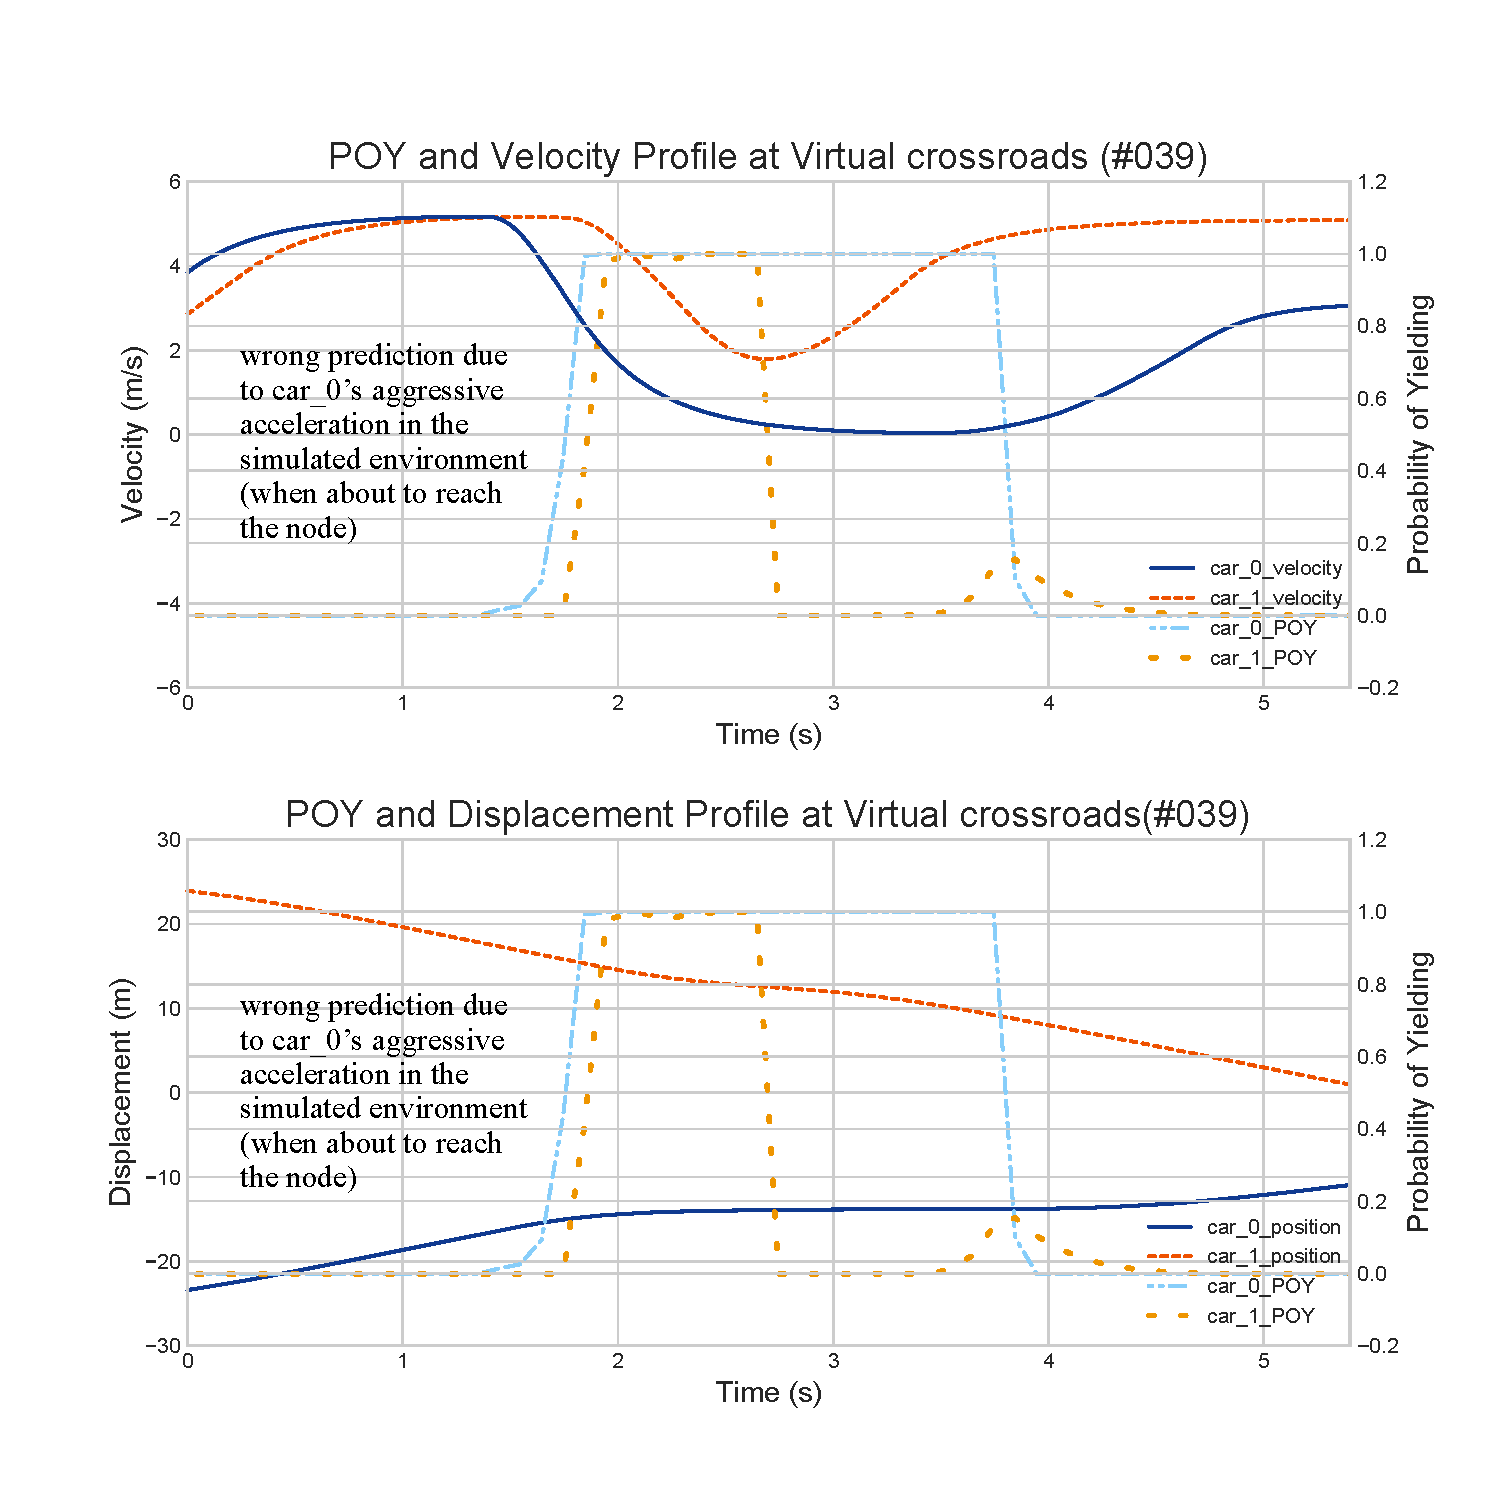
\includegraphics[width=0.85\paperwidth]{trial_039_toosoon.pdf}}
\end{center}
\caption{Example of aggressive driving pattern in simulated environment. where car\_1 begun to accelerate before car\_0 passed the node, causing the false prediction.}
\label{fig:trial039} 
\end{figure}

Comparing to other few behavior prediction model, the $R_{\mathrm{CA}}$ of the proposed model is comparable to the state-of-the-art. In the work of Graf et al. \cite{Graf2014}, the $R_{\mathrm{CA}}$ reached 0.81 at around $T_{\mathrm{minus}} = 3$, while in the proposed model 0.81 is reached at $T_{\mathrm{minus}} = 1.5$. This is owing to the relatively short interaction time span in the simulated environment, where participants tend to send out maximum command velocity. In the literature, interactions at real crossroads takes about 6 secs to cross a 12 to 18 meters long distance, yet at the simulated crossroad, it only takes about 3.5 secs to cross 20 meters. Furthermore, the method proposed in the literature requires pre-trained model for a specific where in POY no training steps are needed. The proposed POY also has the potential of generating better predictions if the parameters characterizing his or her driving pattern is known.


In this section, a novel driver behaviors model at crossroads was proposed. Driver intentions were predicted based on the parameter TTC, which is an important and well developed risk estimation method in traffic safety assessment. Derived form the concept, the TFA distribution was shown to be an innovative and effective driver intentions indicator that can be used to predict the driver behaviors. The normally distributed TFA distribution was then formulated and proven to be an unerring approximation. At last the driver behaviors model was finally proposed and validated at the simulated crossroad where prediction accuracy was comparable to the state-of-the-art driver behaviors prediction method. 

\newpage